\documentclass[11pt,letterpaper]{article}
\usepackage{etch-math}
\usepackage{etch-schematic}
% definitions share the theorem/lemma counter, so no two results collide
\makeatletter
\@ifundefined{c@definition}{}{\let\c@definition\c@lemma \let\thedefinition\thelemma}
\makeatother
\usepackage{graphicx}
\usepackage[section]{placeins}

% Captions were set at \small; at 11pt body that reads as fine print under a
% full-width figure. \normalsize keeps the italic + upright-bold label, which is
% what distinguishes a caption from body text here, and gives back the size.
\captionsetup{font={normalsize,it}}

% ---- paper-specific notation ----
\newcommand{\Gom}{\Gamma_{\Omega}}          % Gindikin cone gamma
\newcommand{\Gc}{\mathcal{G}}               % continued symbol: \Gc_h(r,s)
\newcommand{\Fh}{F_h}
\newcommand{\Zt}{\zeta_2}
\newcommand{\Zint}{\mathbb{Z}}
\newcommand{\Rr}{\mathbb{R}}
\newcommand{\Cc}{\mathbb{C}}
\newcommand{\Qq}{\mathbb{Q}}
\newcommand{\Nn}{\mathbb{N}}
\newcommand{\Reg}{\operatorname{Reg}}
\newcommand{\Rm}{R}                          % shift quotient R_{r,h}
\DeclareMathOperator{\Real}{Re}
\DeclareMathOperator{\rank}{rank}

\hypersetup{
  pdftitle={The Barnes--Gindikin Symbol at Fractional Rank: Continuation Without a Determinant Carrier, Positivity Without a Cone},
  pdfauthor={John Zachary Fitch},
  pdfsubject={Barnes double gamma functions, Gindikin gamma products, Jack polynomials},
  pdfkeywords={Barnes double gamma function, Gindikin gamma, symmetric cone, rank continuation, zeta regularization, Bernstein--Sato polynomial, Wallach set, Jack polynomial, z-measure}
}

\begin{document}

\begin{center}
\estitle{The Barnes--Gindikin Symbol at Fractional Rank:\\Continuation Without a
Determinant Carrier, Positivity Without a Cone}\\[10pt]
{\normalsize John Zachary Fitch}\\[2pt]
{\footnotesize Independent Researcher}\\[1pt]
{\footnotesize\ttfamily zack@internetuniverse.org}\\[1pt]
{\footnotesize ORCID \href{https://orcid.org/0009-0007-7953-1531}{0009-0007-7953-1531}}\\[3pt]
{\footnotesize\itshape September 2026}
\end{center}

\esrule

\begin{abstract}
\noindent
Fix $h>0$. We use the Barnes double zeta to continue the cone-normalized
$N$-factor Gindikin gamma product in its factor count, obtaining a meromorphic
symbol $\Gc_h(r,s)$ on $\Cc^{2}$. At $r=N\in\Zint_{\ge0}$ it recovers the
classical product exactly, and it satisfies rank addition and reflection,
commuting rank and spectral shifts, and reciprocal-step covariance. Its spectral
unit-shift quotient is rational exactly for $r\in\Zint$ and polynomial exactly
for $r\in\Zint_{\ge0}$; consequently no polynomial Bernstein--Sato datum
affine-compatible with this quotient exists away from the nonnegative integer
lattice. We classify all entire multipliers preserving the cocycle and both unit
shifts, determine their behaviour under reciprocal steps, and show that a
sectorial large-$s$ ratio normalization selects $\Gc_h$ uniquely.

Writing $d=2h$, we then study a formal Jack--Riesz pairing with the same rank and
step parameters. Each pivot is the product of one cell polynomial evaluated at
$rd/2$ and at $s$, and its chamber interiors are fixed-rank slices of the Jack
$z$-measure complementary series. At positive nonintegral rank the Wallach ray
becomes bounded. When $\tfrac d2(\lceil r\rceil-r)$ is integral we determine the
exact finite-cutoff erosion staircase; for every rational $d/2$ we prove finite
stabilization; and partition conjugation gives the duality
\begin{equation*}
  (r,d,s)\;\longmapsto\;\Bigl(-\tfrac{rd}{2},\ \tfrac4d,\ -\tfrac{2s}{d}\Bigr).
\end{equation*}
\medskip
\noindent
{\footnotesize\textbf{Keywords.} Barnes double gamma; Gindikin gamma; rank
continuation; Bernstein--Sato polynomial; Wallach set; Jack polynomial; Jack
$z$-measure.}

\smallskip
\noindent
{\footnotesize\textbf{2020 Mathematics Subject Classification.}
Primary 33B15, 11M32;
Secondary 05E05, 11M35, 11S90, 17C20, 32M15, 33C52, 43A85.}
\end{abstract}

\esrule

\section{Introduction}

\subsection{The Gindikin Product Uses Rank in Two Different Ways}

Let $\Omega$ be an irreducible symmetric cone, the cone of squares of a Euclidean
Jordan algebra of rank $N$ and Peirce multiplicity $d$. Its Riesz--Gindikin
integral evaluates to a product of $N$ gamma factors whose arguments descend by
the step $h:=d/2$:
\begin{equation}
  \Gom(s) \;=\; (2\pi)^{\,d\binom{N}{2}/2}\,\prod_{j=0}^{N-1}\Gamma\!\bigl(s-j\tfrac{d}{2}\bigr)
  \;=\; (2\pi)^{\,h\binom{N}{2}}\,\prod_{j=0}^{N-1}\Gamma(s-jh),
  \label{eq:gindikin}
\end{equation}
a formula of Gindikin, in the symmetric-cone form of Faraut and Kor\'anyi
\cite{FK,Gindikin}.

The integer $N$ occurs twice in \eqref{eq:gindikin}, playing a different role
each time. One is geometric: $N$ is the rank of a Jordan algebra, an integer constrained by
the classification. The other is combinatorial: $N$ is the number of factors in a
product. Every other quantity in \eqref{eq:gindikin} varies continuously; only
the length of the product is pinned to an integer. Throughout Part~I, $N$ denotes
a nonnegative integer factor count and $r$ a complex factor count; in Part~II, $R$
denotes an integer cone rank and $N$ the degree cutoff.

This paper continues the second. Fix $h>0$ and let $r$ be a complex variable in
place of the factor count. We construct a function $\Gc_h(r,s)$, meromorphic on
$\Cc^2$, agreeing with \eqref{eq:gindikin} at every $r=N\in\Zint_{\ge0}$, and
determine which parts of its structure survive. No Jordan algebra is claimed to
exist at nonintegral $r$.

The problem is not continuation in $s$, which is classical --- each fixed-length
product is already meromorphic in $s$ --- nor continuation of a
Gindikin--Koecher gamma in a tuple of spectral parameters, treated by Ding, Gross
and Richards \cite{DGR}. It is continuation in the length of the product, with
the spacing $h$ held fixed.

\subsection{Barnes Regularization Continues Only the Factor Count}

A product of gamma factors is the exponential of a sum of logarithms, and a sum
whose length is to be made complex is what zeta regularization handles. Writing
$\log\Gamma$ by the Lerch formula as a derivative of the Hurwitz zeta, the
descending sum $\sum_{j=0}^{r-1}\log\Gamma(s-jh)$ becomes a difference of
derivatives at $z=0$ of the Barnes double zeta $\Zt(z,a\mid 1,h)$, and that
difference continues in $r$ without obstruction. Fixing the branch, the sign of
the zeta derivative, and the power of $2\pi$ once and for all
(Section~\ref{sec:norm}) gives the symbol $\Gc_h(r,s)$, which we call the
\emph{Barnes--Gindikin symbol}.

The normalization is the one used for Shintani--Barnes gamma functions by
Friedman and Ruijsenaars \cite{FR} and, over rational cones, by Tizzano and
Winding \cite{TW,Winding}. What is new is reading the result as a function of
the factor count.

\subsection{Termination and Positivity Test Different Realizability Questions}

The construction and its exact identities come first. \Cref{thm:intspec} shows
\begin{equation*}
  \Gc_h(N,s)\;=\;(2\pi)^{h\binom{N}{2}}\prod_{j=0}^{N-1}\Gamma(s-jh)
  \qquad\text{at every } N\in\Zint_{\ge0},
\end{equation*}
so \eqref{eq:gindikin} is recovered exactly --- not
by a fit through sampled points, but as a consequence of a telescoping identity
for the double zeta together with Lerch's theorem. Cutting and rescaling the
regularized interval then produce the identities the rest of the paper rests on
(Section~\ref{sec:cocycle}): splitting at an interior rank gives the rank-addition
cocycle
\begin{equation}
  \Gc_h(r+q,\,s)\;=\;(2\pi)^{h r q}\,\Gc_h(r,s)\,\Gc_h(q,\,s-rh),
  \label{eq:cocycle-intro}
\end{equation}
the same normalization gives a reflection law
$\Gc_h(-r,s)\,\Gc_h(r,\,s+rh)=(2\pi)^{h r^2}$ across $r=0$, and rescaling the
Barnes lattice gives the reciprocal-step identity of \Cref{thm:duality} relating
$\Gc_h$ to $\Gc_{1/h}$. These, with the two unit shifts of \Cref{thm:shift}, hold
as identities in the continuous variables. The multiplier ambiguity they leave is
then classified rather than assumed away: \Cref{thm:ambiguity} determines every
entire deformation preserving the cocycle and both unit shifts as a rank
character $e^{2\pi ikr}$ times a coboundary of a doubly periodic profile,
\Cref{prop:charcouple} shows that reciprocal covariance couples the two character
indices, and \Cref{bcor:ratio} closes uniqueness against a sectorial large-$s$
normalization. We therefore claim canonicity relative to stated axioms, not a
unique continuation.

Termination is what distinguishes integral rank, and it is what a determinant
carrier would have to reproduce. The unit-step quotient of $\Gc_h$ in $s$ is the
single gamma ratio $\Rm_{r,h}(s)=h^r\,\Gamma(s/h+1)/\Gamma(s/h+1-r)$;
\Cref{thm:term} shows it is rational in $s$ exactly for $r\in\Zint$ and polynomial
exactly for $r\in\Zint_{\ge0}$, while nonintegral $r$ leaves two infinite
arithmetic progressions of poles and zeros that never meet. For a Jordan
determinant of rank $N$ and multiplicity $d$ the Bernstein--Sato polynomial is
$b(s)=\prod_{j=0}^{N-1}(s+1+j\tfrac{d}{2})$ \cite{FK,Kimura}, and
\Cref{prop:bernstein} converts termination into nonexistence: a Bernstein--Sato
polynomial compatible with the shift law, in the precise affine sense of
\eqref{eq:affinecompat}, forces the rank to be a nonnegative integer, negative
integers excluded along with the nonintegral ranks. The symbol exists analytically
at every complex rank; what fails off the nonnegative integer lattice, under the
affine compatibility condition \eqref{eq:affinecompat}, is a polynomial
determinant carrier reproducing the spectral shift quotient. The one place a
degenerate carrier might have supplied the missing step is settled by computation:
\Cref{prop:sextonion} obtains the multiplicity-four $b$-function for the cubic
norm of $J_3(\mathbb{S})$, so that carrier does not realize the formal step $d=6$
either.

The continuation is analytic rather than geometric. Away from nonnegative integer
rank, its recurrence no longer terminates to the polynomial data carried by a
Jordan determinant. But the loss of a determinant does not force positivity to
disappear. The same affine factors can still be assembled into a formal
Jack--Riesz pairing, and this pairing remains positive semidefinite for a genuine
range of spectral parameters even though no symmetric cone lies behind it.

At integer rank, the positive set is the familiar Wallach set: a discrete ladder
followed by an unbounded ray. At fractional rank, that ray is cut off and replaced
by a bounded arrangement of intervals and isolated points. The contents of Young
diagrams record where signs change, which modes become null, and how the
arrangement evolves as partitions of higher degree are admitted. We give a
complete description when the naturally scaled distance to the next integer is
integral, prove that the arrangement eventually stops changing whenever the step
$d/2$ is rational, and show that partition conjugation carries the entire picture
across the duality $d\leftrightarrow 4/d$.

\subsection{Relation to Barnes Products, Bernstein--Sato Theory,
  and Jack \texorpdfstring{$z$}{z}-Measures}

Zeta-regularized products, Barnes multiple gamma functions, cone-indexed
multiple gamma functions, and their cocycle-type functional equations are all
established \cite{Barnes,FR,TW,Winding,PerezMarco}. To our knowledge, however,
the continuation of the \emph{number of Gindikin factors} away from the integer
cone rank, with the Peirce step held fixed, has not appeared. The $b$-function
normalization we use is the classical one of Faraut--Kor\'anyi together with the
prehomogeneous classification of Kimura, cited precisely where used.

The positivity half of the paper runs directly into an existing literature. The cell
products controlling the positivity analysis in Sections~\ref{sec:wallach}--\ref{sec:dual} are the weights of the Jack
$z$-measures of Borodin and Olshanski \cite{BO}, and two of the mechanisms used
there --- strict chamber positivity and the conjugation symmetry --- are their
results read on a fixed-rank slice. \Cref{prop:zmeasure} makes the identification
precise and Section~\ref{sec:zmeasures} isolates what does not follow from it:
the closed semidefinite loci at fixed rank, the finite-degree erosion, the
classification at integral defect, and the exact stabilization degree.

The argument proceeds in three stages. Sections~\ref{sec:norm}--\ref{sec:uniqueness}
construct the symbol, recover the integer product, derive its functional
equations, detect integrality through termination, exclude fractional polynomial
determinant carriers, and fix the continuation by spectral normalization.
Sections~\ref{sec:wallach}--\ref{sec:arith} turn positivity into a question about
the contents of Young diagrams. Section~\ref{sec:dual} transports the resulting
loci across reciprocal steps, and Section~\ref{sec:scope} states the separation
the two halves establish.

\begin{center}
  \essubtitle{Part I. Analytic Continuation and Carrier Obstructions}
\end{center}
\esrule

\section{Barnes Regularization Makes the Factor Count Meromorphic}
\label{sec:norm}

Everything downstream is stated relative to a single fixed choice of Barnes
double zeta function, branch, and regularization. We fix it here and never vary
it. The choice is the Shintani--Barnes convention of Friedman and
Ruijsenaars \cite{FR}, cross-checked against the rational-cone conventions of
Tizzano--Winding \cite{TW}; nothing in the construction is left to an invisible
normalization factor.

\subsection{The Double Zeta Continues the Descending Logarithmic Sum}

\begin{definition}[Barnes double zeta and its regularized log-gamma]
\label{def:barnes}
Fix a step $h>0$. For $\Real(a)>0$, the Barnes double zeta with quasi-periods
$1$ and $h$ is
\begin{equation}
  \Zt(z,a\mid 1,h) \;=\; \sum_{m,n\ge 0}(a+m+nh)^{-z},
  \qquad \Real(z)>2,
  \label{eq:doublezeta}
\end{equation}
with the principal logarithm in every complex power. The sum continues
meromorphically in $z$ to all of $\Cc$ for each fixed $a$ with $\Real(a)>0$, and
continues in $a$ along paths avoiding the lattice $-(\Zint_{\ge0}+h\Zint_{\ge0})$;
for general complex $z$ the powers have branch points there, so the continuation
in $a$ is single-valued on the cut plane, or on the universal cover of its
complement, rather than meromorphic on $\Cc$. What becomes meromorphic after
exponentiation is the symbol of \Cref{def:symbol}. The regularized logarithm of
the double zeta is its $z$-derivative at the origin,
\begin{equation}
  \Fh(a) \;=\; \left.\partial_z\,\Zt(z,a\mid 1,h)\right|_{z=0}.
  \label{eq:Fdef}
\end{equation}
\end{definition}

Its single-variable analogue is the Lerch evaluation of $\log\Gamma$. Writing
$\zeta_H(z,a)=\sum_{m\ge 0}(a+m)^{-z}$ for the Hurwitz zeta, that evaluation
reads
\begin{equation}
  \partial_z\,\zeta_H(z,a)\big|_{z=0} \;=\; \log\Gamma(a)-\tfrac12\log(2\pi).
  \label{eq:lerch}
\end{equation}
The double zeta \eqref{eq:doublezeta} is built to make $\Fh$ the two-index
analogue, and the regularized descending product is defined through it.

\subsection{Cone Normalization Produces a Single-Valued Meromorphic Symbol}

\begin{definition}[The Barnes--Gindikin symbol]
\label{def:symbol}
For a rank $r$ and a spectral shift $s$, the regularized descending interval of
log-gamma values is defined to be
\begin{equation}
  \Reg\sum_{j=0}^{r-1}\log\Gamma(s-jh)
  \;:=\;
  \Fh(s+h-rh)-\Fh(s+h)+\tfrac{r}{2}\log(2\pi).
  \label{eq:reginterval}
\end{equation}
The symbol itself is built from two ingredients, each single-valued. The
\emph{Barnes factor} is
\begin{equation}
  B_h(a)\;=\;\exp\Fh(a),
  \qquad \Real a>0,
  \label{eq:barnesfactor}
\end{equation}
with its standard meromorphic continuation in $a$, and the \emph{cone exponent}
is
\begin{equation}
  A_h(r)\;=\;\frac r2+\frac{h\,r(r-1)}{2}.
  \label{eq:coneexponent}
\end{equation}
The symbol is the corresponding power of $2\pi$ times the Barnes ratio:
\begin{equation}
  \boxed{\;
  \Gc_h(r,s)\;=\;(2\pi)^{A_h(r)}\,
  \frac{B_h(s+h-rh)}{B_h(s+h)}\;}
  \label{eq:symbol}
\end{equation}

Then $\Gc_h$ is meromorphic on $\Cc^2$; no branch data are attached to it,
because none are needed. Its \emph{logarithm} is the only multivalued object
here, and on any simply connected open set that avoids the divisor it admits the
lift
\begin{equation}
  \log\Gc_h(r,s)
  \;=\;
  \Fh(s+h-rh)-\Fh(s+h)+A_h(r)\log(2\pi).
  \label{eq:logG}
\end{equation}
Every functional equation below is a global identity of meromorphic functions;
its logarithmic version is read on a common local lift.
\end{definition}

The two terms of $A_h$ are kept separate and named: $\tfrac r2\log(2\pi)$ is the
Lerch constant of \eqref{eq:lerch} summed along the interval, and
$\tfrac{hr(r-1)}{2}\log(2\pi)$ is the cone prefactor matching the $(2\pi)$-power
of the Gindikin product \eqref{eq:gindikin}.

\begin{remark}
Reduction of a double zeta to a Barnes gamma can in general carry an additive
polynomial in the logarithm \cite[Prop.~3.2]{FR}; fixing all three components of
\eqref{eq:logG} explicitly, rather than absorbing them into an overall constant,
is what makes the cocycle and reflection laws below close exactly, with no
residual constant left over.
\end{remark}

\section{Integer Factor Counts Recover the Gindikin Product Exactly}
\label{sec:intspec}

The continuation has the following exact specialization, obtained directly from
the difference equation of the double zeta together with the Lerch formula.


\begin{theorem}{Integer specialization}{intspec}
For every nonnegative integer $N$,
\begin{equation}
  \Gc_h(N,s)\;=\;(2\pi)^{\,h N(N-1)/2}\,\prod_{j=0}^{N-1}\Gamma(s-jh).
  \label{eq:intspec}
\end{equation}
In particular $\Gc_h$ reproduces the Gindikin product \eqref{eq:gindikin} on the
nonnegative integers, with the empty product giving $\Gc_h(0,s)=1$.
\end{theorem}

\begin{proof}[Proof of \Cref{thm:intspec}]
The argument telescopes the double zeta and then applies the Lerch formula a
single time.

\step{telescoping the double zeta}
Shifting the index $n\mapsto n+1$ in \eqref{eq:doublezeta} removes the row
$n=0$, so in the region of absolute convergence
\begin{equation}
  \Zt(z,a\mid 1,h)-\Zt(z,a+h\mid 1,h)\;=\;\sum_{m\ge 0}(a+m)^{-z}\;=\;\zeta_H(z,a),
  \label{eq:telescope-one}
\end{equation}
and both sides continue meromorphically in $z$, so \eqref{eq:telescope-one}
persists by analytic continuation. Iterating \eqref{eq:telescope-one} $N$ times
gives
\begin{equation}
  \Zt(z,a\mid 1,h)-\Zt(z,a+Nh\mid 1,h)
  \;=\;\sum_{k=0}^{N-1}\zeta_H(z,a+kh).
  \label{eq:telescope-N}
\end{equation}

\step{differentiating at zero}
Apply $\partial_z|_{z=0}$ to \eqref{eq:telescope-N} and use the Lerch
formula~\eqref{eq:lerch} on each of the $N$ summands on the right:
\begin{equation}
  \Fh(a)-\Fh(a+Nh)
  \;=\;\sum_{k=0}^{N-1}\Bigl(\log\Gamma(a+kh)-\tfrac12\log(2\pi)\Bigr).
  \label{eq:diffzero}
\end{equation}

\step{substitution and assembly}
Put $a=s+h-Nh$, so that $a+Nh=s+h$ and, as $k$ runs from $0$ to $N-1$, the
arguments $a+kh=s-(N-1-k)h$ run through the set $\{s-jh:0\le j\le N-1\}$.
Identity \eqref{eq:diffzero} then reads
\begin{equation*}
  \Fh(s+h-Nh)-\Fh(s+h)
  \;=\;\sum_{j=0}^{N-1}\log\Gamma(s-jh)\;-\;\tfrac{N}{2}\log(2\pi).
\end{equation*}
Substituting this into the definition~\eqref{eq:logG} at $r=N$, the
$-\tfrac{N}{2}\log(2\pi)$ cancels the Lerch term $+\tfrac{N}{2}\log(2\pi)$ and
leaves
\begin{equation*}
  \log\Gc_h(N,s)
  \;=\;\sum_{j=0}^{N-1}\log\Gamma(s-jh)\;+\;\tfrac{h N(N-1)}{2}\log(2\pi),
\end{equation*}
which is \eqref{eq:intspec} after exponentiation. The Lerch formula
\eqref{eq:lerch} is the only analytic input, and the telescoping
\eqref{eq:telescope-one}--\eqref{eq:telescope-N} is exact; no step depends on
the size of $N$.
\end{proof}

\begin{remark}
The proof isolates where continuity in $r$ comes from: the left-hand side of
\eqref{eq:diffzero} is $\Fh(s+h-rh)-\Fh(s+h)$ with $r=N$, and that expression is
already meromorphic in a \emph{complex} $r$. Integer specialization is the
statement that on the integers this analytic object coincides with the finite
product; the content of the paper is what the same object does between the
integers.
\end{remark}

\section{Exact Functional Equations Arise from Cutting and Rescaling
  the Regularized Interval}
\label{sec:cocycle}

The structural core of the construction is a family of functional equations.
They are not asymptotic, and they are not inferred from matching the symbol at
integer ranks: they are exact relations among the regularized
intervals~\eqref{eq:logG}, holding as meromorphic identities in all complex
variables. The mechanism is a single observation, rendered in
Figure~\ref{fig:split}: a descending product of gamma factors can be cut at an
interior point.

\subsection{Cutting the Interval Gives the Rank Cocycle}

\begin{theorem}{Interval splitting gives the rank cocycle}{cocycle}
The Barnes--Gindikin symbol satisfies, for all $r,q,s\in\Cc$,
\begin{align}
  \Gc_h(r+q,\,s)&\;=\;(2\pi)^{\,h r q}\,\Gc_h(r,s)\,\Gc_h(q,\,s-rh),
  \label{eq:cocycle}\\[2pt]
  \Gc_h(-r,\,s)\,\Gc_h(r,\,s+rh)&\;=\;(2\pi)^{\,h r^2}.
  \label{eq:reflection}
\end{align}
Both are global identities of meromorphic functions.
\end{theorem}

\begin{figure}[htbp]
\centering
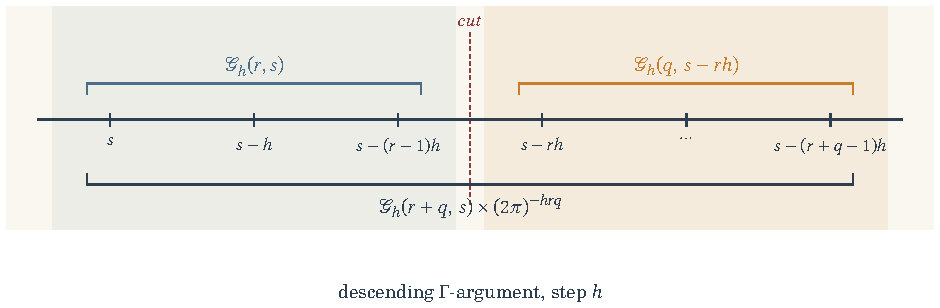
\includegraphics{figs/fig1-cocycle-split.pdf}
\caption{The cocycle is an interval split, the two shaded spans being the two
factors. Drawn at integer $r$ and $q$, where
the picture is literal: the descending gamma arguments of $\Gc_h(r{+}q,s)$ break
at the cut $s-rh$ into the $r$ factors of $\Gc_h(r,s)$ and the $q$ factors of
$\Gc_h(q,s-rh)$. The shift $s\mapsto s-rh$ in the second symbol is exactly the
position of the cut, and the mismatch in the $(2\pi)$-bookkeeping across it is
the cross-term $(2\pi)^{hrq}$. At complex $r,q$ there is no factor count to
draw; what persists is \eqref{eq:cocycle}, the meromorphic continuation of this
identity.}
\label{fig:split}
\end{figure}

\begin{proof}[Proof of \Cref{thm:cocycle}]
Write $B=B_h$. The Barnes ratio of \eqref{eq:symbol} telescopes:
\begin{equation}
  \frac{B(s+h-(r+q)h)}{B(s+h)}
  \;=\;
  \frac{B(s+h-rh)}{B(s+h)}\cdot
  \frac{B\bigl((s-rh)+h-qh\bigr)}{B\bigl((s-rh)+h\bigr)} ,
  \label{eq:telescoperatio}
\end{equation}
the second quotient being exactly the one occurring in $\Gc_h(q,s-rh)$. For the
prefactor, the cone exponent $A_h$ of \eqref{eq:coneexponent} obeys the addition
rule
\begin{equation}
  A_h(r+q)-A_h(r)-A_h(q)\;=\;h\,rq,
  \label{eq:Aadd}
\end{equation}
since the linear part of $A_h$ is additive and
$\tfrac h2\bigl[(r+q)^2-(r+q)-r^2+r-q^2+q\bigr]=hrq$. Multiplying
\eqref{eq:telescoperatio} by $(2\pi)^{A_h(r+q)}$ and inserting \eqref{eq:Aadd}
gives \eqref{eq:cocycle}.

For the reflection, put $q=-r$ in \eqref{eq:cocycle}. Then $\Gc_h(0,s)=1$
directly from \eqref{eq:symbol}, so
\begin{equation*}
  1=(2\pi)^{-hr^{2}}\,\Gc_h(r,s)\,\Gc_h(-r,\,s-rh),
\end{equation*}
which is exactly the reflection law \eqref{eq:reflection}.

No logarithm was taken anywhere above, so no branch was chosen; the logarithmic
forms of \eqref{eq:cocycle} and \eqref{eq:reflection} hold on any common simply
connected lift.
\end{proof}

\subsection{Commuting Rank and Spectral Shifts Produces the Shift Quotient}

\begin{theorem}{Rank and spectral shifts commute}{shift}
For all $r,s\in\Cc$, as meromorphic identities,
\begin{align}
  \frac{\Gc_h(r,s+1)}{\Gc_h(r,s)}
  &\;=\;\Rm_{r,h}(s),
  \qquad
  \Rm_{r,h}(s)\;:=\;h^{\,r}\,
  \frac{\Gamma\!\bigl(\tfrac{s}{h}+1\bigr)}{\Gamma\!\bigl(\tfrac{s}{h}+1-r\bigr)},
  \label{eq:rankmeter}\\[2pt]
  \frac{\Gc_h(r+1,s)}{\Gc_h(r,s)}
  &\;=\;(2\pi)^{\,hr}\,\Gamma(s-rh).
  \label{eq:rshift}
\end{align}
The two are compatible: $\Rm_{r+1,h}(s)/\Rm_{r,h}(s)=s-rh$.
\end{theorem}

\begin{proof}[Proof of \Cref{thm:shift}]
Deleting the row $m=0$ from \eqref{eq:doublezeta} and rescaling the remaining
lattice by $h$ gives the second difference equation of the double zeta,
\begin{equation}
  \Zt(z,a\mid 1,h)-\Zt(z,a+1\mid 1,h)
  \;=\;\sum_{n\ge 0}(a+nh)^{-z}
  \;=\;h^{-z}\,\zeta_H\!\bigl(z,\tfrac{a}{h}\bigr).
  \label{eq:mdiff}
\end{equation}
Differentiating at $z=0$ and using $\zeta_H(0,x)=\tfrac12-x$ together with the
Lerch formula~\eqref{eq:lerch},
\begin{equation}
  \Fh(a)-\Fh(a+1)
  \;=\;\log\Gamma\!\bigl(\tfrac{a}{h}\bigr)-\tfrac12\log(2\pi)
  +\Bigl(\tfrac{a}{h}-\tfrac12\Bigr)\log h .
  \label{eq:Fdiff}
\end{equation}
Apply \eqref{eq:Fdiff} at the two endpoints $a_1=s+h-rh$ and $a_2=s+h$ of
\eqref{eq:logG}. The prefactor $A(r)\log(2\pi)$ does not depend on $s$ and
cancels, the two Lerch constants cancel against each other, and the $\log h$
terms combine to $(a_2-a_1)h^{-1}\log h=r\log h$. What remains is
\begin{equation*}
  \log\Gc_h(r,s+1)-\log\Gc_h(r,s)
  \;=\;\log\frac{\Gamma\bigl(\tfrac{s}{h}+1\bigr)}{\Gamma\bigl(\tfrac{s}{h}+1-r\bigr)}
  +r\log h,
\end{equation*}
which is \eqref{eq:rankmeter}. For \eqref{eq:rshift}, put $q=1$ in the
cocycle~\eqref{eq:cocycle} and use $\Gc_h(1,x)=\Gamma(x)$ from
\Cref{thm:intspec}. The compatibility relation follows from
$\Gamma(x+1)=x\Gamma(x)$ with $x=\tfrac{s}{h}-r$.
\end{proof}

We call $\Rm_{r,h}$ the \emph{shift quotient}. It is not an auxiliary construction:
by \eqref{eq:rankmeter} it \emph{is} the unit-step quotient of the symbol in the
spectral variable, so any realization of $\Gc_h$ by a shift-invariant model must
reproduce it. Sections~\ref{sec:term} and~\ref{sec:bernstein} exploit exactly
that. The compatibility relation is a discrete zero-curvature condition: the
$r$-update and the $s$-update commute, which is the local counterpart of the
cocycle.

A third functional equation relates the symbol at reciprocal steps. It is not a
consequence of the cocycle, and it couples different values of $h$.

\subsection{Rescaling the Barnes Lattice Sends \texorpdfstring{$h$}{h} to \texorpdfstring{$1/h$}{1/h}}

\begin{theorem}{Rescaling the Barnes lattice sends $h$ to $1/h$}{duality}
Write $Q_h(a)=\Zt(0,a\mid 1,h)=\dfrac{a^{2}}{2h}-\dfrac{(1+h)a}{2h}
+\dfrac{h^{2}+3h+1}{12h}$. Then
\begin{equation}
  \Fh(a)\;=\;F_{1/h}\!\bigl(\tfrac{a}{h}\bigr)-\log h\cdot Q_h(a),
  \label{eq:Fduality}
\end{equation}
and consequently
\begin{equation}
  \Gc_h(r,s)\;=\;(2\pi)^{(1-h)r}\;
  h^{\,rs+\frac{r(h-1)}{2}-\frac{h r^{2}}{2}}\;
  \Gc_{1/h}\!\bigl(hr,\;\tfrac{s}{h}+1-\tfrac1h\bigr).
  \label{eq:Gduality}
\end{equation}
The powers of $h>0$ use the real logarithm; the resulting formula is a
meromorphic identity in $r$ and $s$.
\end{theorem}

\begin{proof}[Proof of \Cref{thm:duality}]
Every lattice point of \eqref{eq:doublezeta} factors as
$a+m+nh=h\bigl(\tfrac{a}{h}+\tfrac{m}{h}+n\bigr)$, so
$\Zt(z,a\mid1,h)=h^{-z}\,\Zt\bigl(z,\tfrac{a}{h}\mid \tfrac1h,1\bigr)$, and
$\Zt$ is symmetric in its two quasi-periods. Evaluating at $z=0$ gives
$Q_h(a)=\Zt(0,\tfrac{a}{h}\mid1,\tfrac1h)$, and differentiating at $z=0$ gives
\eqref{eq:Fduality}. Substituting \eqref{eq:Fduality} at the two endpoints of
\eqref{eq:logG}, matching $\tfrac{s}{h}+1$ against the upper endpoint of the
reciprocal symbol and $\tfrac{s}{h}+1-r$ against its lower endpoint, identifies
the reciprocal rank as $hr$ and the reciprocal shift as $\tfrac{s}{h}+1-\tfrac1h$;
collecting the residual $Q_h$ difference and the prefactor exponents gives the
elementary cofactor in \eqref{eq:Gduality}.
\end{proof}

\begin{remark}
\label{rem:duality-scope}
Reciprocity couples the $h$ and $1/h$ columns without removing the periodic
ambiguity at either step. Writing $h=p/q$ in lowest terms, the fundamental profiles of
Section~\ref{sec:uniqueness} transform covariantly: at
$u=\tfrac{s}{h}+1-\tfrac1h$ one has $2\pi p\,u=2\pi q\,s+2\pi(p-q)$ with
$p-q\in\Zint$, so a profile of period $1/q$ at step $h$ is carried to a profile
of period $1/p$ at step $1/h$, and the associated deformations correspond under
\eqref{eq:Gduality}. The two periodic coboundary spaces are therefore in
bijection. On the discrete part, however, reciprocity is a genuine constraint:
it couples the two rank characters, and \Cref{prop:charcouple} computes the
coupling.
\end{remark}


\section{Polynomial Termination Detects Nonnegative Integral Rank}
\label{sec:term}

The Barnes--Gindikin symbol remains nonrational in the spectral variable even
at positive integral rank. Its spectral unit-shift quotient behaves differently:
it is rational exactly at integral rank and polynomial exactly at nonnegative
integral rank. This section isolates that termination phenomenon.

The object to examine is the shift quotient $\Rm_{r,h}$ of \eqref{eq:rankmeter},
which \Cref{thm:shift} identifies as the unit-step quotient of $\Gc_h$ in $s$.
It is the falling-factorial content of the Gindikin product: at a nonnegative
integer $r=N$ the gamma ratio is the descending factorial
$(\tfrac{s}{h})(\tfrac{s}{h}-1)\cdots(\tfrac{s}{h}-N+1)$, and the prefactor
$h^{N}$ clears denominators to give $\prod_{j=0}^{N-1}(s-jh)$ --- exactly the
product of arguments carried by $\Gc_h(N,s)$ in \eqref{eq:intspec}, stripped of
its gamma envelope. That is the piece a genuine determinant would have to
reproduce, and Section~\ref{sec:bernstein} uses it in that role. Its virtue here
is that its analytic type in $s$, rational or not, is a clean detector, and the
dichotomy proved below comes from a competition between two lattices of poles and
zeros, shown in Figure~\ref{fig:divisor}.


\begin{theorem}{The shift quotient terminates exactly at integral rank}{term}
Fix $h>0$. The shift quotient $\Rm_{r,h}$ is a rational function of $s$ if and
only if $r\in\Zint$, and a polynomial in $s$ if and only if $r\in\Zint_{\ge 0}$.
Explicitly, for $N\in\Zint_{\ge 0}$,
\begin{equation}
  \Rm_{N,h}(s)\;=\;\prod_{j=0}^{N-1}(s-jh),
  \qquad
  \Rm_{-N,h}(s)\;=\;\frac{1}{\displaystyle\prod_{k=1}^{N}(s+kh)}\quad(N\ge 1),
  \label{eq:term-explicit}
\end{equation}
so negative integers give the reciprocal-polynomial branch. For $r\notin\Zint$,
$\Rm_{r,h}$ is not rational in $s$: it has infinitely many poles and
infinitely many zeros.
\end{theorem}

\begin{figure}[htbp]
\centering
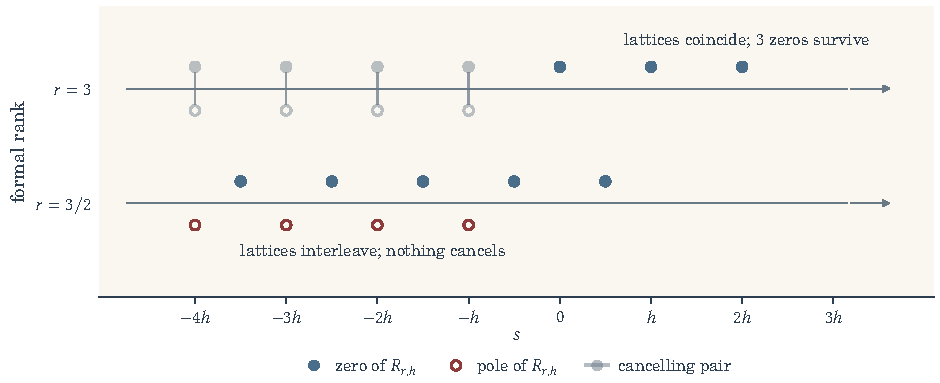
\includegraphics{figs/fig2-divisor-cancellation.pdf}
\caption{Termination is divisor cancellation. Zeros are drawn on the upper tier
of each row and poles on the lower, so coincidence of the two lattices is
vertical alignment and failure of coincidence is a visible stagger. The shift
quotient $\Rm_{r,h}$ carries a pole lattice, at $-h,-2h,\dots$ from the numerator, and a zero lattice, at
$h(r{-}1),h(r{-}2),\dots$ from the reciprocal denominator. At integer $r$ the
two share the grid $h\Zint$, the negative tails coincide and cancel, and
finitely many zeros survive, so $\Rm_{r,h}$ is a polynomial when
$r\in\Zint_{\ge0}$ and reciprocal-polynomial when $r$ is a negative integer. At nonintegral $r$
the zero lattice sits on a different coset of $h\Zint$, the tails interleave
without cancelling, and infinitely many poles and zeros remain.}
\label{fig:divisor}
\end{figure}

\begin{proof}[Proof of \Cref{thm:term}]
The prefactor $h^{r}$ is a nonzero constant in $s$ and affects neither
rationality nor the divisor, so we argue with the gamma ratio.

\step{the integer branches}
For $r=N\ge 0$, repeated application of $\Gamma(x+1)=x\,\Gamma(x)$ gives
$\Gamma(\tfrac{s}{h}+1)/\Gamma(\tfrac{s}{h}+1-N)=\prod_{j=0}^{N-1}(\tfrac{s}{h}-j)$;
multiplying by $h^N$ then yields the left identity of \eqref{eq:term-explicit},
a polynomial of degree $N$, the empty product at $N=0$ being $1$. For $r=-N$ with
$N\ge 1$, the recurrence in the other direction gives
$\Gamma(\tfrac{s}{h}+1)/\Gamma(\tfrac{s}{h}+1+N)=1/\prod_{k=1}^{N}(\tfrac{s}{h}+k)$,
and multiplying by $h^{-N}$ yields the right identity, which is rational and
reciprocal-polynomial but not a polynomial.

\step{the converse, by divisor}
Write $x=s/h$. The numerator $\Gamma(x+1)$ contributes poles of $\Rm_{r,h}$ at
$x=-1,-2,-3,\dots$, i.e.\ at $s\in\{-h,-2h,-3h,\dots\}$. The reciprocal
denominator $1/\Gamma(x+1-r)$ contributes zeros at $x+1-r=0,-1,-2,\dots$, i.e.\
at $s\in\{h(r-1),h(r-2),h(r-3),\dots\}$. These are two arithmetic progressions
with common difference $h$: the poles lie on the coset $h\Zint$, the zeros on the
coset $h(r-1)+h\Zint$. The two cosets coincide exactly when $r-1\in\Zint$, that
is when $r\in\Zint$; then the deep-negative tails of the two progressions agree
term for term and cancel, leaving only finitely many uncancelled points ---
which \Cref{thm:term}'s integer branches identify. When $r\notin\Zint$ the two
cosets are disjoint, so no pole meets any zero; both progressions survive in
full, and $\Rm_{r,h}$ has infinitely many poles and zeros. A nonzero rational
function on the Riemann sphere has only finitely many of each, so $\Rm_{r,h}$ is
not rational. This is a statement about the whole meromorphic function, not about
a finite sample of values.
\end{proof}


\section{Polynomial Bernstein Quotients Exclude Fractional Determinant Carriers}
\label{sec:bernstein}

\subsection{Jordan Determinants Realize the Terminated Shift Quotient}
\label{sec:bfunction}

The symbol $\Gc_h(r,s)$ exists, as an analytic object, at every complex rank,
and so does its shift quotient. The termination theorem says that the shift
quotient is rational only at integral rank and polynomial only at nonnegative
integral rank. This section draws the structural consequence: a nonintegral rank
cannot be the rank of a \emph{determinant}, in a sense made precise through the
theory of Bernstein--Sato $b$-functions. The result is a no-go theorem; its
scope is fixed once, after \Cref{prop:bernstein}.

For a simple Euclidean Jordan algebra of rank $N$ and Peirce multiplicity $d$,
the determinant $\Delta$ is a relative invariant of the structure group, and its
Bernstein--Sato identity is classical \cite[Prop.~VII.1.4]{FK}: writing the
identity with the standard exponent $s+1$ on the input,
\begin{equation}
  \Delta^{*}(\partial)\,\Delta^{s+1}\;=\;b(s)\,\Delta^{s},
  \qquad
  b(s)\;=\;\prod_{j=0}^{N-1}\Bigl(s+1+j\tfrac{d}{2}\Bigr).
  \label{eq:bfunction}
\end{equation}
The $b$-function is a polynomial of degree exactly $N$, its roots the arithmetic
progression $-1,\,-1-\tfrac{d}{2},\,\dots,\,-1-(N-1)\tfrac{d}{2}$. For the Albert
algebra, where $(N,d)=(3,8)$, this is $(s+1)(s+5)(s+9)$, the entry recorded in
Kimura's classification of the exceptional $27$-dimensional determinant
\cite[Prop.~2.22, entry (27)]{Kimura}; the formal step $d=6$ at rank $3$ would
give $(s+1)(s+4)(s+7)$. The step $\tfrac{d}{2}=h$ of the $b$-function's roots is the
same step that governs the shift quotient's divisor, and the coincidence is exact
rather than approximate: comparing \eqref{eq:bfunction} with the integer
specialization $\Rm_{N,h}(u)=\prod_{j=0}^{N-1}(u-jh)$ of \Cref{thm:term} at
$u=-s-1$ gives
\begin{equation}
  b(s)\;=\;(-1)^{N}\,\Rm_{N,h}(-s-1)
  \qquad (N\in\Zint_{\ge0}).
  \label{eq:b-is-shift}
\end{equation}
The classical $b$-function is thus the shift quotient itself, read backwards
through the affine substitution $u=-s-1$. That identification is what makes the
compatibility hypothesis of \Cref{prop:bernstein} a description of the classical
situation rather than a condition invented to force the result.

\Needspace*{14\baselineskip}
\subsection{Polynomiality Forces Nonnegative Integral Rank}

The obstruction is best stated for the shift quotient alone, with no auxiliary
notion of carrier. Any realization compatible with the shift
law is then covered by a single corollary, and nothing is assumed that makes the
conclusion automatic.

\begin{proposition}{Polynomial Bernstein quotients force nonnegative integral rank}{bernstein}
Fix $h>0$ and $r\in\Cc$. Suppose there are a nonzero polynomial
$b\in\Cc[u]$ and constants $a,c\in\Cc^{\times}$, $\beta\in\Cc$, with
\begin{equation}
  b(u)\;=\;c\,\Rm_{r,h}(au+\beta)
  \label{eq:affinecompat}
\end{equation}
as meromorphic functions of $u$. Then $r=N\in\Zint_{\ge0}$ and $\deg b=N$.
\end{proposition}

\begin{proof}[Proof of \Cref{prop:bernstein}]
A nondegenerate affine substitution $u\mapsto au+\beta$ with $a\ne0$, followed by
multiplication by $c\ne0$, is invertible on meromorphic functions and preserves
both polynomiality and degree. Hence \eqref{eq:affinecompat} holds with $b$
polynomial exactly when $\Rm_{r,h}$ is polynomial, and then
$\deg b=\deg\Rm_{r,h}$. By \Cref{thm:term} that happens precisely for
$r=N\in\Zint_{\ge0}$, in which case the degree is $N$.
\end{proof}

\begin{corollary}
\label{cor:carrier}
Let $f$ be a polynomial determinant, or more generally a relative invariant of a
prehomogeneous vector space, whose Bernstein--Sato polynomial $b_f$ is compatible
with the Barnes--Gindikin shift quotient in the sense of \eqref{eq:affinecompat}
for some $r$. Then $r$ must be a nonnegative integer, and $\deg b_f=r$. Jordan
determinants and prehomogeneous relative invariants are the principal examples,
but no such structure is required of $f$.
\end{corollary}

The classical Jordan determinant satisfies \eqref{eq:affinecompat} exactly: by
\eqref{eq:b-is-shift} the
classical Jordan determinant of a rank-$N$ simple Euclidean Jordan algebra
saturates \eqref{eq:affinecompat} exactly, with $a=-1$, $\beta=-1$ and
$c=(-1)^{N}$. What \Cref{prop:bernstein} adds is that no other value of $r$ can
do so. Both directions of the integer condition are used: nonintegral $r$ is
excluded by the infinitude of the divisor, and negative integral $r$ is excluded
because the quotient inverts to a product of linear forms.

The scope of the obstruction, stated once. It concerns polynomial
Bernstein--Sato data affine-compatible with the shift quotient, and it constrains
the \emph{formal} rank appearing in the shift law rather than any dimension or
rank of an underlying algebra. It does not exclude operator-algebraic, quotient,
GNS, or nonpolynomial realizations; indeed Section~\ref{sec:wallach} exhibits a
genuine positive-semidefinite form at fractional rank, which some construction of that
kind may well organize.

\begin{remark}[Why the sextonionic cubic requires a separate computation]
\label{rem:bs-open}
The obstruction above routes through termination and the classical
prehomogeneous $b$-function, both established results. It does \emph{not}
include a from-scratch Bernstein--Sato computation for a degenerate cubic. The
sextonionic Hermitian space $J_3(\mathbb{S})$ is the natural test: a
$21$-dimensional carrier of structural rank $3$ whose cubic norm is degenerate.
The radical of its polarized cubic is the six-dimensional ideal
$A_3(\mathbb{H}^{\perp})$; equivalently, the cubic factors through the
fifteen-dimensional semisimple quotient. That carrier distinguishes structural
rank from formal multiplicity, and for it the $b$-function can be computed
outright. The computation is next, in two steps: first a general lemma about
irrelevant variables, then its application to $J_3(\mathbb{S})$.
\end{remark}

\subsection{The Sextonionic Cubic Factors Through the Quaternionic Quotient}

\Needspace*{9\baselineskip}
\begin{boxedlemma}{Adjoining irrelevant variables does not change the $b$-function}{dummy}
Let $g\in\Cc[x_1,\dots,x_m]\setminus\{0\}$, and regard it as the element
$f(x,y)=g(x)$ of the larger ring $\Cc[x_1,\dots,x_m,y_1,\dots,y_n]$. Then
$b_f=b_g$.
\end{boxedlemma}

\begin{proof}[Proof of \Cref{blem:dummy}]
Let $B_g,B_f\subset\Cc[\sigma]$ be the two Bernstein ideals; for the general
theory of Bernstein ideals and $b$-functions see \cite[Ch.~1]{Bjork}.

If $P(x,\partial_x,\sigma)g^{\sigma+1}=b(\sigma)g^{\sigma}$, the same operator,
acting trivially in the $y$ variables, gives
$P(x,\partial_x,\sigma)f^{\sigma+1}=b(\sigma)f^{\sigma}$, so $B_g\subseteq B_f$.

Conversely let $Q(x,y,\partial_x,\partial_y,\sigma)f^{\sigma+1}
=b(\sigma)f^{\sigma}$. Write $Q$ in \emph{normal order}, every $\partial_y$
placed to the right of every coefficient:
\begin{equation*}
  Q=\sum_{\gamma}Q_\gamma(x,y,\partial_x,\sigma)\,\partial_y^{\gamma}.
\end{equation*}
Every element of the Weyl algebra admits such a form, and the reordering is
where the argument is actually made: $\partial_yy=y\partial_y+1$, so a term
written with $\partial_y$ on the left does not differentiate in $y$ last. Once $Q$ is normally ordered, each $\gamma\ne0$ annihilates $f^{\sigma+1}$,
because $f$ does not depend on $y$. Hence
$Q_0(x,y,\partial_x,\sigma)g^{\sigma+1}=b(\sigma)g^{\sigma}$, and evaluating the
polynomial coefficients at any fixed $y=y_0$ gives a Bernstein identity for $g$,
so $b\in B_g$. The two Bernstein ideals therefore coincide, and so do their
monic generators.
\end{proof}

\begin{proposition}{The sextonionic cubic has the quaternionic $b$-function}{sextonion}
Work over $\Cc$. Let $\mathbb{S}$ be the sextonion algebra, let
\begin{equation*}
  \pi\colon J_3(\mathbb{S})\longrightarrow J_3(\mathbb{H})
\end{equation*}
be the quotient by its six-dimensional square-zero radical
$A_3(\mathbb{H}^{\perp})$ \cite[Def.~3.1]{Westbury}, \cite[\S8.2]{LM}, and let
$f$ and $g$ be the corresponding determinantal cubics. Then $f=g\circ\pi$ up to a
nonzero scalar, and consequently
\begin{equation}
  b_f(\sigma)\;=\;b_g(\sigma)\;=\;(\sigma+1)(\sigma+3)(\sigma+5)
  \;=\;\prod_{j=0}^{2}\Bigl(\sigma+1+j\tfrac{4}{2}\Bigr).
  \label{eq:bsextonion}
\end{equation}
The sextonionic cubic therefore carries the multiplicity-four Bernstein
progression and does not realize the formal multiplicity $d=6$, for which
\eqref{eq:bfunction} would give $(\sigma+1)(\sigma+4)(\sigma+7)$.
\end{proposition}

\begin{proof}[Proof of \Cref{prop:sextonion}]
Write $\mathbb{S}=\mathbb{H}\oplus N$ with $N=\mathbb{H}^{\perp}$ the
two-dimensional Cayley module, $N\cdot N=0$, norm $n(q+\eta)=n(q)$ and
conjugation $\overline{q+\eta}=\bar q-\eta$ \cite[Def.~3.1]{Westbury}. Then $N$ is
the radical of the polar form and the trace $t(x)=x+\bar x$ kills $N$.

Write $a_i=q_i+\eta_i$ for the three off-diagonal entries. In the cubic norm
\begin{equation*}
  f=x_1x_2x_3-\sum_{i}x_i\,n(a_i)+t\bigl((a_1a_2)a_3\bigr)
\end{equation*}
the norm term is unchanged by $a_i\mapsto a_i+\eta_i$ because $N$ is totally
isotropic and orthogonal to $\mathbb{H}$ for the polar form. For the trace term,
$N$ is an ideal with $N\cdot N=0$, so a product of three elements at least one of
which lies in $N$ again lies in $N$; every element of $N$ has zero trace, so
$t((a_1a_2)a_3)$ is unchanged as well. Hence $f$ is constant along the six
directions spanned by the $\eta_i$, which is exactly
$A_3(\mathbb{H}^{\perp})=\ker\pi$, and $f=g\circ\pi$ with $g$ the cubic norm of
$J_3(\mathbb{H})$.

In coordinates adapted to the splitting, the six radical directions do not occur
in $f$ at all. \Cref{blem:dummy} therefore gives $b_f=b_g$, a nonzero scalar
being irrelevant to a monic Bernstein--Sato polynomial. Finally $J_3(\mathbb{H})$
is simple Euclidean of rank $3$ and Peirce multiplicity $d=4$, so
\eqref{eq:bfunction} evaluates $b_g$ as the right-hand side of
\eqref{eq:bsextonion}.
\end{proof}

The carrier therefore distinguishes structural rank from formal multiplicity
without producing a new multiplicity: it has structural rank $3$, its cubic is
genuinely degenerate, and its $b$-function is nonetheless the one belonging to
$d=4$. The formal step $d=6$ at rank $3$ is not realized here, and by
\Cref{prop:bernstein} it could only be realized by an object whose shift quotient
is a polynomial of degree $3$, which pins the rank but not the multiplicity.

\section{Spectral Normalization Selects a Symbol from the Full Ambiguity Class}
\label{sec:uniqueness}

The functional equations do not determine the continuation without an additional
normalization. We first classify their holomorphic logarithmic deformations, then
impose the two unit shifts and the integer-rank data. This isolates the periodic
ambiguity at rational $h$, its disappearance at irrational $h$ for a fixed
logarithmic lift, and the function-level characters that remain. We then analyse
growth and prove uniqueness under a spectral ratio normalization.

\subsection{Integer Values Alone Do Not Determine the Continuation}

Agreement on integer ranks alone gives no useful uniqueness: additive tails such
as $\Gc_h(r,s)+\sin(2\pi r)$ vanish on the lattice and are unconstrained off it.
Since the cocycle~\eqref{eq:cocycle} is multiplicative, a deformation with any
chance of preserving it must act multiplicatively as well,
\begin{equation}
  \widetilde{\Gc}_h(r,s)\;=\;\Gc_h(r,s)\,\exp\bigl(E(r,s)\bigr),
  \label{eq:deform}
\end{equation}
and it is the exponent $E$, not an additive tail, that must satisfy the additive
form~\eqref{eq:addcocycle} of the cocycle. Asked in this form, the question has a complete
answer.

\subsection{Every Entire Deformation Is a Character Times a Periodic Coboundary}

Before exhibiting deformations we record that the coboundary form is not a
choice: it is forced.

\begin{lemma}[Classification of additive cocycles]
\label{lem:coclass}
Let $E:\Cc^{2}\to\Cc$ be entire and satisfy
\begin{equation}
  E(r+q,s)=E(r,s)+E(q,s-rh),\qquad E(0,s)=0 .
  \label{eq:addcocycle}
\end{equation}
for all $r,q,s\in\Cc$. Then $E(r,s)=\varphi(s)-\varphi(s-rh)$ for an entire
$\varphi$, unique up to an additive constant.
\end{lemma}

\begin{proof}[Proof of \Cref{lem:coclass}]
Differentiate \eqref{eq:addcocycle} in $q$ at $q=0$ and set
$a(s)=\partial_rE(0,s)$; the left side gives $\partial_rE(r,s)$ and the right
gives $a(s-rh)$, so $\partial_rE(r,s)=a(s-rh)$. Since $a$ is entire and $\Cc$ is simply connected, there is an entire $\varphi$
with $\varphi'=a/h$. Then
$\partial_r\bigl[\varphi(s)-\varphi(s-rh)\bigr]=h\varphi'(s-rh)=a(s-rh)$, and
both $E(r,s)$ and $\varphi(s)-\varphi(s-rh)$ vanish at $r=0$. Two entire functions of $r$ with the same
derivative and the same value at $r=0$ coincide. For uniqueness, if $\varphi_1$
and $\varphi_2$ give the same cocycle then $\psi=\varphi_1-\varphi_2$ satisfies
$\psi(s)=\psi(s-rh)$ for all $r,s$; as $rh$ ranges over $\Cc$, $\psi$ is
invariant under every translation and hence constant.
\end{proof}

The classification is stated for an additive exponent, and the reduction of an
arbitrary entire multiplicative factor to that form is not an assumption but a
consequence of the cocycle.

\begin{lemma}[Every entire multiplicative cocycle has an entire logarithm]
\label{lem:mult2add}
Let $h>0$ and let $H\in\mathcal{O}(\Cc^{2})$ satisfy
\begin{equation}
  H(r+q,s)=H(r,s)\,H(q,s-rh),\qquad H(0,s)=1 .
  \label{eq:multcocycle}
\end{equation}
Then $H=e^{E}$ for an entire $E$ satisfying the additive
cocycle~\eqref{eq:addcocycle}.
\end{lemma}

\begin{proof}[Proof of \Cref{lem:mult2add}]
Taking $q=-r$ in \eqref{eq:multcocycle} gives $H(r,s)H(-r,s-rh)=H(0,s)=1$, so
$H$ vanishes nowhere on $\Cc^{2}$. Then $dH/H$ is a closed holomorphic $1$-form
on the simply connected $\Cc^{2}$, hence has a primitive: $H=e^{E_0}$ with $E_0$
entire. Since $e^{E_0(0,s)}=H(0,s)=1$, the function $E_0(0,\cdot)$ takes values
in $2\pi i\Zint$ and is continuous, hence equal to a single constant $2\pi in$;
put $E=E_0-2\pi in$, so that $H=e^{E}$ and $E(0,s)=0$. The cocycle defect
\begin{equation*}
  \delta(r,q,s)\;=\;E(r+q,s)-E(r,s)-E(q,s-rh)
\end{equation*}
is entire on $\Cc^{3}$ and satisfies $e^{\delta}=1$ by \eqref{eq:multcocycle},
so it takes values in the discrete set $2\pi i\Zint$ and is therefore constant.
At $q=0$ it equals $-E(0,s-rh)=0$, so $\delta\equiv0$ and $E$ satisfies
\eqref{eq:addcocycle}.
\end{proof}

\begin{theorem}{Complete fixed-step entire ambiguity}{ambiguity}
Let $h>0$. By \Cref{lem:mult2add} every entire multiplicative deformation of
$\Gc_h$ preserving the rank-addition cocycle~\eqref{eq:cocycle} is $e^{E}$ for an
entire $E$ satisfying~\eqref{eq:addcocycle}; let $E$ be such a function and set
$\widetilde{\Gc}_h(r,s)=\Gc_h(r,s)e^{E(r,s)}$.
Suppose $\widetilde{\Gc}_h$ satisfies the same two exponentiated unit-shift
equations as $\Gc_h$. Then there are an integer $k$ and an entire $\psi$ with
\begin{equation}
  \psi(s+1)=\psi(s),\qquad \psi(s+h)=\psi(s),
  \label{eq:bothperiods}
\end{equation}
such that
\begin{equation}
  E(r,s)\;=\;2\pi ikr+\psi(s)-\psi(s-rh).
  \label{eq:ambiguity}
\end{equation}
Conversely, every $E$ of this form preserves the rank-addition
cocycle~\eqref{eq:cocycle}, the reflection~\eqref{eq:reflection}, both
exponentiated unit-shift equations, and every value $\Gc_h(N,s)$ with
$N\in\Zint$.

If the unit shifts are imposed as exact identities of a fixed logarithmic lift,
then $k=0$. If $h=p/q$ in lowest terms, the admissible $\psi$ are exactly the
entire functions of period $1/q$, modulo constants. If $h\notin\Qq$, then $\psi$
is constant, so the only function-level deformations are the rank characters
$e^{2\pi ikr}$, and the fixed logarithmic lift is rigid.
\end{theorem}

\begin{proof}[Proof of \Cref{thm:ambiguity}]
\Cref{lem:coclass} gives an entire $\varphi$, unique modulo an additive
constant, with $E(r,s)=\varphi(s)-\varphi(s-rh)$; the constant cancels from the
difference.

\step{the $s$-shift}
Write $\Delta_1\varphi(s)=\varphi(s+1)-\varphi(s)$. Preserving the exponentiated
$s$-shift equation of \Cref{thm:shift} amounts to the requirement that
\begin{equation*}
  \exp\bigl(\Delta_1\varphi(s)-\Delta_1\varphi(s-rh)\bigr)=1
  \qquad\text{for all }r,s\in\Cc .
\end{equation*}
The exponent is entire in $(r,s)$ and takes values in the discrete set
$2\pi i\Zint$, so it is constant; it vanishes at $r=0$, hence vanishes
identically. As $rh$ ranges over all of $\Cc$, this says that the difference
$\Delta_1\varphi$ is constant:
\begin{equation}
  \varphi(s+1)-\varphi(s)=c,\qquad c\in\Cc .
  \label{eq:phi-unit}
\end{equation}

\step{the $r$-shift}
Preserving the exponentiated $r$-shift equation means
$\exp\bigl(\varphi(z)-\varphi(z-h)\bigr)=1$ for all $z\in\Cc$, by the same
computation applied to $z=s-rh$. The entire function $\varphi(z)-\varphi(z-h)$
therefore has image in $2\pi i\Zint$ and is constant:
\begin{equation}
  \varphi(z+h)-\varphi(z)=2\pi ik,\qquad k\in\Zint .
  \label{eq:phi-rank}
\end{equation}

\step{splitting off the character}
Put $\psi(z)=\varphi(z)-\tfrac{2\pi ik}{h}z$. By \eqref{eq:phi-rank} $\psi$ has
period $h$, so its restriction to $\Rr$ is bounded, $h$ being positive and real.
By \eqref{eq:phi-unit},
$\psi(z+1)-\psi(z)=c-\tfrac{2\pi ik}{h}$ is constant, and iterating the unit
increment $n$ times gives $\psi(x+n)-\psi(x)=n\bigl(c-\tfrac{2\pi ik}{h}\bigr)$,
which is unbounded in $n$ unless the constant vanishes. Hence $\psi$ has period
$1$ as well, and
\begin{equation*}
  E(r,s)=\varphi(s)-\varphi(s-rh)
        =\tfrac{2\pi ik}{h}\bigl(s-(s-rh)\bigr)+\psi(s)-\psi(s-rh)
        =2\pi ikr+\psi(s)-\psi(s-rh),
\end{equation*}
which is the asserted form \eqref{eq:ambiguity}.

\step{the converse and the three specializations}
For the converse, $2\pi ikr$ is a coboundary for the linear profile
$\varphi(s)=2\pi iks/h$ and $\psi(s)-\psi(s-rh)$ is one for $\psi$, so both are
additive cocycles and \Cref{lem:coclass} applies in reverse; the cocycle and
reflection identities hold for any coboundary, and \eqref{eq:bothperiods} gives
back both unit shifts after exponentiation. At $r=N\in\Zint$ the character
contributes $e^{2\pi ikN}=1$ and the periodic part contributes
$\psi(s)-\psi(s-Nh)=0$, so $\widetilde{\Gc}_h$ agrees with $\Gc_h$ at every
integer rank.

If the unit shifts are imposed on a fixed lift, the lifted increment
$E(r+1,s)-E(r,s)=2\pi ik+\psi(s-rh)-\psi(s-rh-h)=2\pi ik$ must vanish, so $k=0$.
If $h=p/q$ with $\gcd(p,q)=1$, the group generated by $1$ and $h$ is
$q^{-1}\Zint$, and \eqref{eq:bothperiods} says exactly that $\psi$ has period
$1/q$; conversely every entire $1/q$-periodic $\psi$ has both periods. If $h$ is
irrational, $\Zint+h\Zint$ is dense in $\Rr$, so the entire $\psi$ is constant on
a dense subset of $\Rr$ modulo translation, hence constant, and only the rank
characters survive.
\end{proof}

\Cref{thm:ambiguity} settles in one statement the two questions that the
algebraic package leaves open, and it separates them cleanly. The rank character
$e^{2\pi ikr}$ is invisible to every exponentiated identity and to every
integer-rank value, and it is killed only by requiring the unit shifts of a fixed
logarithmic lift; it is not killed by fixing the lift at $r=0$, since $2\pi ikr$
also vanishes there. The periodic coboundary is the genuinely arithmetic part: at
$h=p/q$ it is a full function space, at irrational $h$ it is nothing at all. Every
geometric Peirce step $h=d/2$ is rational, so the geometric cases are exactly the
ones carrying the ambiguity.

The two recurrences in \eqref{eq:bothperiods} impose invariance under the
subgroup $\Zint+h\Zint$. Neither period condition can be discarded uniformly in
$h$, although one may imply the other when one period is an integral multiple of
the other: at $h=\tfrac12$, $h$-periodicity implies unit periodicity, whereas
unit periodicity need not imply $h$-periodicity. A profile of period $1$ but not
of period $\tfrac12$ preserves the $s$-recurrence while failing the
$r$-recurrence and the integer-rank values. This is why the family survives all
four algebraic constraints at once, and it is what distinguishes it from the
additive witnesses above. For $h=p/q$ the profiles
\begin{equation}
  \psi(s)=\varepsilon\sin(2\pi qs),
  \qquad
  \psi(s)=\varepsilon\cos(2\pi qs)
  \label{eq:profiles}
\end{equation}
are nonconstant of period exactly $1/q$, so the deformation is genuinely
nontrivial off the lattice: with $\varepsilon=1$ the exponent attains
$E=2$, its extremal value on the real locus, since the two sine terms in
\eqref{eq:ambiguity} can take opposite signs. As an entire function of two
complex variables it has no global extremum.

\subsection{Reciprocal Covariance Couples the Remaining Character Indices}
\label{sec:charcouple}

The reciprocal-step identity of \Cref{thm:duality} is not consumed by the
classification just proved: it acts on the classified family. On the periodic
part it acts covariantly, carrying profiles to profiles, as
\Cref{rem:duality-scope} records. On the discrete part it is a genuine
constraint, and the constraint is arithmetic.

\begin{proposition}{Reciprocal covariance couples the character indices}{charcouple}
Let $h>0$ and let $H_h(r,s)=e^{2\pi ik_hr}$, $H_{1/h}(r',s')=e^{2\pi ik_{1/h}r'}$
be rank characters at the two steps, with $k_h,k_{1/h}\in\Zint$. The deformed
pair $\widetilde{\Gc}_h=\Gc_hH_h$ and $\widetilde{\Gc}_{1/h}=\Gc_{1/h}H_{1/h}$
satisfies \eqref{eq:Gduality} with the same elementary cofactor if and only if
\begin{equation}
  H_h(r,s)\;=\;H_{1/h}\!\Bigl(hr,\;\tfrac{s}{h}+1-\tfrac1h\Bigr),
  \label{eq:charcompat}
\end{equation}
that is, if and only if
\begin{equation}
  k_h\;=\;h\,k_{1/h}.
  \label{eq:charcouple}
\end{equation}
Consequently, if $h=p/q$ in lowest terms then
\begin{equation}
  (k_h,k_{1/h})\;=\;(pm,\,qm),\qquad m\in\Zint,
  \label{eq:charlattice}
\end{equation}
so the admissible index pairs form the rank-one lattice $\Zint\cdot(p,q)$ inside
$\Zint^{2}$; and if $h\notin\Qq$ then $k_h=k_{1/h}=0$.
\end{proposition}

\begin{proof}[Proof of \Cref{prop:charcouple}]
Dividing the deformed instance of \eqref{eq:Gduality} by the undeformed one
cancels the cofactor and the two symbols and leaves exactly
\eqref{eq:charcompat}. Evaluated on the two characters it reads
$e^{2\pi ik_hr}=e^{2\pi ik_{1/h}hr}$ for all $r\in\Cc$; the difference of the
two entire exponents takes values in $2\pi i\Zint$, hence is constant, and it
vanishes at $r=0$, so $k_h=hk_{1/h}$. For $h=p/q$ with $\gcd(p,q)=1$,
\eqref{eq:charcouple} reads $qk_h=pk_{1/h}$, so $p\mid k_h$; writing $k_h=pm$
gives $k_{1/h}=qm$, and every such pair satisfies \eqref{eq:charcouple}. If $h$
is irrational then $k_h=hk_{1/h}$ with both indices integral forces
$k_{1/h}=0$, hence $k_h=0$.
\end{proof}

So reciprocity does constrain the classified family, though only through its
discrete part. The periodic coboundary spaces at the two steps remain in
bijection, exactly as \Cref{rem:duality-scope} says; what the reciprocal step
pins down is the pair of rank characters, to a rank-one lattice at rational
step and to nothing at all at irrational step. That is the function-level
counterpart of the rigidity already recorded in \Cref{thm:ambiguity}.

\subsection{Fundamental Coboundaries Reveal the Finer Zero Lattice}

Because the family is explicit, its growth can be computed rather than
estimated, and this is what converts the obstruction from a qualitative remark
into a quantitative one.

\begin{proposition}{Fundamental coboundaries vanish on a finer rank lattice}{cbtype}
Let $h=p/q$ in lowest terms, take the profiles \eqref{eq:profiles} with
$\varepsilon=1$, and write $E_\varphi$ for either of the two resulting
logarithmic deformations $E_{\cos}$ and $E_{\sin}$. Then for all complex $r,s$,
\begin{align}
  E_{\cos}(r,s)&=-2\,\sin\bigl(\pi q rh\bigr)\,\sin\bigl(\pi q(2s-rh)\bigr),\notag\\
  E_{\sin}(r,s)&=\phantom{-}2\,\sin\bigl(\pi q rh\bigr)\,\cos\bigl(\pi q(2s-rh)\bigr),
  \label{eq:cbfactor}
\end{align}
so the two profiles share the common envelope $\sin(\pi q rh)$, and they
satisfy the $s$-free identity
\begin{equation}
  E_{\cos}(r,s)^2+E_{\sin}(r,s)^2\;=\;4\sin^2\bigl(\pi q rh\bigr).
  \label{eq:cbinvariant}
\end{equation}
Consequently:
\begin{enumerate}
\item[(i)] $E_\varphi(r,s)=0$ for \emph{every} $s$ exactly when $r\in\tfrac1p\Zint$;
  this is the common envelope zero set of the two-profile family, and an
  individual profile carries further $s$-dependent phase zeros;
\item[(ii)] along the ray $r=Re^{i\theta}$,
\begin{equation}
  \limsup_{R\to\infty}\frac{1}{R}\log\bigl|E_\varphi(Re^{i\theta},s)\bigr|
  \;=\;2\pi qh\,\lvert\sin\theta\rvert\;=\;2\pi p\,\lvert\sin\theta\rvert,
  \label{eq:cbtype}
\end{equation}
the ordinary limit existing whenever $\sin\theta\neq0$ and failing on both real
rays $\theta=0$ and $\theta=\pi$, where $E_\varphi$ is a bounded function of $R$
with infinitely many zeros. Thus each of the two fundamental logarithmic
deformations $E_{\cos}$ and $E_{\sin}$ has exponential type $2\pi p$ in the
interpolation variable, depending only on the \emph{numerator} of $h$. More
generally, the $n$-th Fourier mode has type $2\pi|n|p$, while an arbitrary
periodic entire profile need not have finite exponential type.
\end{enumerate}
\end{proposition}

\begin{proof}[Proof of \Cref{prop:cbtype}]
The identities \eqref{eq:cbfactor} are the sum-to-product formulas
\begin{equation*}
  \cos A-\cos B=-2\sin\tfrac{A+B}{2}\,\sin\tfrac{A-B}{2},
  \qquad
  \sin A-\sin B=2\cos\tfrac{A+B}{2}\,\sin\tfrac{A-B}{2},
\end{equation*}
applied with $A=2\pi qs$ and $B=2\pi q(s-rh)$, so that
$\tfrac{A+B}{2}=\pi q(2s-rh)$ and $\tfrac{A-B}{2}=\pi qrh$;
and \eqref{eq:cbinvariant} follows because
$\sin^2+\cos^2=1$ identically. For (i), the second factor of
\eqref{eq:cbfactor} depends on $s$ and the first does not, so vanishing for every
$s$ forces $\sin(\pi qrh)=0$, that is $qrh=rp\in\Zint$. For (ii), put
$w=2s-rh$, so that $\operatorname{Im}w=2\operatorname{Im}s-hR\sin\theta$ while
$\operatorname{Im}(rh)=hR\sin\theta$. As $|\operatorname{Im}\cdot|\to\infty$ both
$|\sin|$ and $|\cos|$ grow like $\tfrac12e^{\pi q|\operatorname{Im}\cdot|}$, so
each factor contributes $\pi qhR|\sin\theta|+O(1)$ and the product contributes
$2\pi qhR|\sin\theta|+O(1)$, with $2\pi qh=2\pi p$. On either real ray, $\theta=0$ or $\theta=\pi$, both imaginary parts remain
bounded, so $|E_\varphi|$ is a bounded function of $R$; by (i) it vanishes
whenever $R\in\tfrac1p\Zint$, while it is not identically zero, so its modulus is
also bounded away from zero along some sequence. The $\limsup$ is therefore $0$
and no ordinary limit exists.
\end{proof}

Part (i) sharpens what agreement at
integer ranks is worth: the periodic-coboundary subfamily of
\Cref{thm:ambiguity} agrees with $\Gc_h$ not merely on $\Zint$ but on the lattice
$\tfrac1p\Zint$, which is $p$ times finer. The rank characters do not, since
$e^{2\pi ikr}$ is generally nontrivial there. Integer agreement is a
considerably weaker constraint than it appears, and this is the precise sense in
which the additive witnesses of the previous subsection are inadequate: they are
valid against interpolation constrained only on the integer lattice, and
insufficient against the full cocycle-compatible package.

Second, $2\pi p$ is the type of the \emph{fundamental} harmonic, not of the
ambiguity space. The admissible profiles form the space of functions of period
$1/q$; its $n$-th Fourier mode $\varphi_n(s)=e^{2\pi i n q s}$ has envelope
$\sin(\pi n q rh)$ and hence type $2\pi|n|p$, and a general periodic entire
profile need not have finite exponential type at all. Thus $2\pi p$ is the least
type occurring among the nonzero Fourier modes, and any statement below about
``the type of the ambiguity'' should be read in that sense. It is in any case an
assertion about the \emph{logarithmic} deformation $E_\varphi$ and about nothing
else. It does not describe $\exp(E_\varphi)$, which
is the multiplicative ambiguity actually acting on $\Gc_h$ and which has infinite
entire order; nor does it describe $\Gc_h$, whose growth is computed in
\Cref{prop:growth} below and is of a different class altogether. Keeping the
three objects apart is essential to the discussion that follows.

For integer $h$ one has $p=h$, so that $2\pi p=\pi d$ with $d=2h$. This is a
restricted arithmetic identity, holding exactly when the reduced denominator
$q$ equals $1$; in general the type is $2\pi p=\pi q d$. We record it because
$d$ also indexes the positivity analysis of Sections~\ref{sec:wallach}--\ref{sec:dual}, but no
causal or independently measured link between the two is claimed, and the
identity fails already at $h=\tfrac12$, where $d=1$ and $2\pi p=2\pi\neq\pi$.
Among simple Euclidean Jordan algebras of rank at least $3$, the Peirce
multiplicities are $d\in\{1,2,4\}$, together with the exceptional value $d=8$
only at rank $3$. Rank-$2$ spin factors realize every integer multiplicity
$d\ge1$ \cite[Ch.~V]{FK}. Thus the pair $(r,d)=(3,6)$ used here is formal,
although $d=6$ does occur for genuine rank-$2$ spin factors.

\begin{remark}[The rate near the real axis]
\label{rem:cusp}
The angular law \eqref{eq:cbtype} degrades as $\theta\to0$, and the
factorization \eqref{eq:cbfactor} locates the transition exactly. For
$b=\operatorname{Im}s>0$, $\sin\theta>0$ and $r=Re^{i\theta}$ the exponential
envelope is
\begin{equation}
  \log|E_\varphi|
  \;=\;\pi q\bigl(hR\sin\theta+\lvert 2b-hR\sin\theta\rvert\bigr)+O(1),
  \label{eq:envelope}
\end{equation}
whose leading radial slope is $0$ for $R<R_2$ and equals
$2\pi qh\sin\theta$ for $R>R_2$, where
\begin{equation*}
  R_2=\frac{2\operatorname{Im}(s)}{h\sin\theta}.
\end{equation*}
The locus
$\operatorname{Im}(s-rh)=0$, at $R_1=\operatorname{Im}(s)/(h\sin\theta)$, is the
midpoint of the leading plateau and not the crossover, which sits at $R_2=2R_1$.
A radial window whose upper limit lies below $R_2$ is therefore entirely
pre-asymptotic, and a rate measured on such a window is not evidence about the
exponential type.
\end{remark}

\subsection{Rank Growth Lies Outside Carlson's Interpolation Class}

The classical route to uniqueness for an interpolation problem is a Carlson-type
theorem \cite[Ch.~9]{Boas}: a function of exponential type less than $\pi$ on the
imaginary axis, bounded on a half-plane, and vanishing on $\Zint_{\ge0}$,
vanishes identically.
Applying it here requires knowing the growth class of the objects involved, and
that is now available in closed form.

One ingredient of the expansion is not proved here. The half-sector computation
below identifies every coefficient from the present normalization, but widening
the sector to the full slit plane is exactly the content of Ruijsenaars's
analysis of the multiple zeta \cite{Ruij}, and the following lemma states what is
imported in the form the proof consumes. The translation between his conventions
and ours is tabulated in \Cref{app:ruij}.

\begin{lemma}[Sectorial continuation of the Barnes remainder]
\label{lem:sector}
Fix $h>0$, $M\ge1$ and $\delta>0$, and let
$\rho_M(z,a)=\Gamma(z)\Zt(z,a\mid1,h)-\sum_{n\le M}c_n(h)\Gamma(z+n)a^{-z-n}$ be
the truncated remainder of \eqref{eq:zetaexp}. Then $\rho_M$, and its derivative
in $z$ at $z=0$, continue holomorphically in $a$ from the right half-sector to
$\Cc\setminus(-\infty,0]$, and
\begin{equation*}
  \partial_z\rho_M(0,a)\;=\;O\bigl(\lvert a\rvert^{-M-1}\bigr)
  \qquad\text{uniformly on } \lvert\arg a\rvert\le\pi-\delta .
\end{equation*}
\end{lemma}

\begin{proof}[Proof of \Cref{lem:sector}]
Specialize \cite[Prop.~2.3 and (3.13)--(3.15)]{Ruij} to $N=2$, $a_1=1$, $a_2=h$
under the identifications of \Cref{app:ruij}. Proposition~2.3 there continues the
remainder \cite[(3.14)]{Ruij} holomorphically to $\Cc\setminus(-\infty,0]$, and
\cite[(3.15)]{Ruij} bounds it by
$O(\lvert a\rvert^{\,N-M'-1})=O(\lvert a\rvert^{-M-1})$ uniformly on
$\lvert\arg a\rvert\le\pi-\delta$, since $M'=M+2$ by \Cref{app:ruij}. The cited
expansion is already the differentiated one, so no further passage through
$\partial_z$ is required.
\end{proof}

\begin{proposition}{The symbol has quadratic-logarithmic rank growth}{growth}
Write $B_n$ for the Bernoulli numbers with the convention $B_1=-\tfrac12$, and
write $B_n(x)$ for the Bernoulli polynomials. Expand the kernel
$\bigl((1-e^{-t})(1-e^{-ht})\bigr)^{-1}$ as $\sum_{n\ge-2}c_n(h)t^n$,
with $c_{-2}=\tfrac1h$, $c_{-1}=\tfrac{1+h}{2h}$, $c_0=\tfrac{h^2+3h+1}{12h}$,
and in general $c_n(h)=\tfrac1h\sum_{j+k=n+2}B_j(1)B_k(1)h^k/(j!\,k!)$. Then,
uniformly on every closed sector $\lvert\arg a\rvert\le\pi-\delta$,
\begin{equation}
  \Fh(a)\;\sim\;-\frac{a^{2}\log a}{2h}+\frac{3a^{2}}{4h}
  +\frac{(1+h)a(\log a-1)}{2h}-\frac{(h^{2}+3h+1)\log a}{12h}
  +\sum_{n\ge1}c_n(h)(n-1)!\,a^{-n}.
  \label{eq:stirling}
\end{equation}
Substituting $a_r=s+h-rh$ into \eqref{eq:logG} gives the rank asymptotic of
$\Gc_h$, uniformly while $a_r$ keeps a fixed angular distance from the negative
real axis, which in the rank plane excludes a translated positive-real ray. In
particular, for fixed $x$, $s$ and $h>0$,
\begin{equation}
  \log\bigl|\Gc_h(x+iT,s)\bigr|
  =\frac{h}{2}T^{2}\log T
  +\frac{h}{2}\Bigl(\log\frac{h}{2\pi}-\frac32\Bigr)T^{2}
  +O(T\log T).
  \label{eq:vertical}
\end{equation}
\end{proposition}

\begin{proof}[Proof of \Cref{prop:growth}]
We first identify the coefficients in a right half-sector, where the Mellin
representation converges. Fix $\varepsilon>0$ and assume
$\lvert\arg a\rvert\le\tfrac{\pi}{2}-\varepsilon$, so that
$\Real a\ge c_\varepsilon\lvert a\rvert>0$. For $\Real z>2$ the double zeta then
has the Mellin representation
\begin{equation}
  \Zt(z,a\mid1,h)=\frac{1}{\Gamma(z)}\int_0^{\infty}
  \frac{t^{z-1}e^{-at}}{(1-e^{-t})(1-e^{-ht})}\,dt ,
  \label{eq:mellin}
\end{equation}
obtained by expanding the geometric series and integrating term by term. Write
$K(t)$ for the kernel and let $K(t)=\sum_{n\ge-2}c_n(h)t^{n}$ be its Laurent
expansion at $t=0$, which converges for $0<t<2\pi\min(1,h^{-1})$ and has the
stated coefficients, since
$t/(1-e^{-t})=\sum_{j\ge0}B_j(1)t^{j}/j!$ gives
$c_n(h)=h^{-1}\sum_{j+k=n+2}B_j(1)B_k(1)h^{k}/(j!\,k!)$.

Fix $M\ge1$ and a compact set $\mathcal{K}\subset\{\Real z>-M-1\}$, and split
\eqref{eq:mellin} as
\begin{equation*}
  \Gamma(z)\Zt(z,a\mid1,h)
  =\int_0^{1}t^{z-1}e^{-at}\Bigl[K(t)-\sum_{n=-2}^{M}c_nt^{n}\Bigr]dt
   +\sum_{n=-2}^{M}c_n\int_0^{1}t^{z+n-1}e^{-at}\,dt
   +\int_1^{\infty}t^{z-1}e^{-at}K(t)\,dt .
\end{equation*}
The first integrand is $O(t^{\Real z+M})$ at the origin, so that term is
holomorphic for $\Real z>-M-1$. The remaining two are controlled by
$\Real a\ge c_\varepsilon\lvert a\rvert$, and only by that: on the contour
$(0,\infty)$ of \eqref{eq:mellin} the factor $e^{-at}$ grows exponentially when
$\Real a<0$, so the estimates of this paragraph are asserted for
$\lvert\arg a\rvert\le\tfrac{\pi}{2}-\varepsilon$ and nowhere else. There, for
$\lvert a\rvert\ge1$, the tail integral is entire in $z$ and obeys the bound
\begin{equation*}
  \int_1^{\infty}t^{z-1}e^{-at}K(t)\,dt
  \;=\;O_{\varepsilon,\mathcal{K}}\bigl(e^{-c_\varepsilon\lvert a\rvert/2}\bigr),
\end{equation*}
uniformly for $z\in\mathcal{K}$, and completing each monomial integral from
$\int_0^{1}$ to $\int_0^{\infty}$ produces $\Gamma(z+n)a^{-z-n}$ together with
an error $\int_1^{\infty}t^{z+n-1}e^{-at}\,dt$ obeying the same bound. Hence,
in the right half-sector $\lvert\arg a\rvert\le\tfrac{\pi}{2}-\varepsilon$,
\begin{equation}
  \Zt(z,a\mid1,h)=\sum_{n=-2}^{M}c_n(h)\frac{\Gamma(z+n)}{\Gamma(z)}a^{-z-n}
   +E_M(z,a),
  \label{eq:zetaexp}
\end{equation}
with $E_M(\,\cdot\,,a)$ holomorphic on $\{\Real z>-M-1\}$ and
\begin{equation*}
  E_M(z,a)=O_{\mathcal{K},h,\varepsilon,M}\bigl(\lvert a\rvert^{-M-1}\bigr)
\end{equation*}
uniformly for $z\in\mathcal{K}$, by Watson's lemma applied to the subtracted
integrand. Because that bound is uniform on a compact neighbourhood of $z=0$,
Cauchy's estimate on a fixed circle about $z=0$ transfers it to the derivative:
\begin{equation}
  \partial_zE_M(0,a)=O_{h,\varepsilon,M}\bigl(\lvert a\rvert^{-M-1}\bigr).
  \label{eq:cauchyrem}
\end{equation}

Differentiate \eqref{eq:zetaexp} at $z=0$ and use
$\Fh(a)=\partial_z\Zt(z,a\mid1,h)\big|_{z=0}$ from \Cref{def:barnes}.
For $n\ge1$ the factor $\Gamma(z+n)/\Gamma(z)=z(z+1)\cdots(z+n-1)$ vanishes to
first order at $z=0$, with derivative $(n-1)!$, contributing
$c_n(h)(n-1)!\,a^{-n}$. For the exceptional indices the factor is a
\emph{reciprocal} of a rising product, and contributes at $z=0$:
\begin{equation}
  \frac{\Gamma(z-2)}{\Gamma(z)}=\frac{1}{(z-1)(z-2)},
  \qquad
  \frac{\Gamma(z-1)}{\Gamma(z)}=\frac{1}{z-1},
  \qquad
  \frac{\Gamma(z)}{\Gamma(z)}=1 .
  \label{eq:gammaratios}
\end{equation}
These take the values $\tfrac12$, $-1$, $1$ and have derivatives
$\tfrac34$, $-1$, $0$ at $z=0$.
Differentiating $c_n(h)\bigl(\Gamma(z+n)/\Gamma(z)\bigr)a^{-z-n}$ at $z=0$, the
factor $a^{-z-n}=e^{-(z+n)\log a}$ supplying the logarithms, therefore gives
$-\tfrac{a^{2}\log a}{2h}+\tfrac{3a^{2}}{4h}$ at $n=-2$,
$\tfrac{(1+h)a(\log a-1)}{2h}$ at $n=-1$ and
$-\tfrac{(h^{2}+3h+1)\log a}{12h}$ at $n=0$, after inserting
$c_{-2}=\tfrac1h$, $c_{-1}=\tfrac{1+h}{2h}$, $c_{0}=\tfrac{h^{2}+3h+1}{12h}$.
These are the first three terms of \eqref{eq:stirling}. With
\eqref{eq:cauchyrem} controlling the tail, this establishes
\eqref{eq:stirling} on every closed right half-sector
$\lvert\arg a\rvert\le\tfrac{\pi}{2}-\varepsilon$.

The extension from the right half-sector to every closed slit sector
$\lvert\arg a\rvert\le\pi-\delta$ is \Cref{lem:sector}. So extended,
\cite[(3.13)]{Ruij} is \eqref{eq:stirling} term for term: its logarithmic
coefficient is $-\tfrac12B_{2,2}(a)$, which is $-Q_h(a)$ for the polynomial
$Q_h$ of \Cref{thm:duality}, and its remaining terms are the three exceptional
terms and the tail $\sum_{n\ge1}c_n(h)(n-1)!\,a^{-n}$ computed above. The
half-sector computation is given in full because it identifies those coefficients
from the present normalization rather than importing them.

For \eqref{eq:vertical}, put $a_r=s+h-rh$ with $r=x+iT$. Then
$a_r=-ihT+O(1)$, so $\lvert a_r\rvert=hT+O(1)$ and
$\arg a_r=-\tfrac{\pi}{2}+O(T^{-1})$, which stays in a fixed subsector.
Taking real parts in \eqref{eq:stirling} through \eqref{eq:logG}, the leading
term contributes $\tfrac h2T^{2}\log(hT)$, the term $3a^{2}/(4h)$ contributes
$-\tfrac{3h}{4}T^{2}$, and the prefactor of \eqref{eq:logG} contributes
$-\tfrac h2T^{2}\log 2\pi$; the remaining terms are $O(T\log T)$. Collecting the
three contributions gives \eqref{eq:vertical}.
\end{proof}

The expansion fixes the growth class of each of the three objects involved.
By \eqref{eq:vertical}, $\Gc_h$ has quadratic-logarithmic growth in the rank
variable: it is not of exponential type at all, so no order-one hypothesis
applies to it, and a slope measured on a finite window of $\log|\Gc_h|$ along a
vertical line describes that window, not an exponential type. The multiplicative
ambiguity $\exp(E_\varphi)$ has infinite entire order, so it lies outside an
order-one theorem as well, even though its logarithm $E_\varphi$ has order one
and type $2\pi p$. Finally, the difficulty is \emph{not} that the classical
threshold $\pi$ is too small: an axiom bounding the relevant type below $\pi$ is
stricter than one bounding it below $2\pi$, and would exclude $E_\varphi$ if it
could legitimately be imposed. What obstructs the argument is the mismatch of
growth classes between the theorem and the objects, not the size of the constant.

The uniformity in \Cref{prop:growth} is genuinely sectorial: along the excluded
ray the remainder degrades rather than averaging away, and no uniform
inverse-power bound survives as the angular distance to that ray shrinks to
zero. Any statement derived from \eqref{eq:stirling} must carry its sector with
it.

\begin{remark}[Log-convexity is not a Bohr--Mollerup substitute]
\label{rem:noconvex}
The one classical route left --- fixing the continuation by log-convexity in the
rank variable, as Bohr--Mollerup fixes $\Gamma$ --- is also unavailable, and a
single exact value settles it. At $h=1$,
\begin{equation}
  \log\Gc_1(2,10)-2\log\Gc_1(1,10)+\log\Gc_1(0,10)=\log\frac{2\pi}{9}<0 ,
  \label{eq:noconvex}
\end{equation}
so one second difference is negative and no global convexity axiom in $r$ can
hold.
\end{remark}

\subsection{Spectral Asymptotics Force Ratio-Normalized Uniqueness}

Growth in the rank variable is not the only route. The unit-step recurrence of
\Cref{thm:shift} is in $s$, and an asymptotic normalization in that variable
settles the question outright. The substantial statement is the expansion; the
uniqueness principle is a one-line consequence of it.

\begin{proposition}{Uniform spectral asymptotics}{spectral}
Fix $h>0$, a compact $K\subset\Cc$, an integer $M\ge1$ and $\delta>0$.
Throughout this proposition $\log\Gc_h$ denotes the lift \eqref{eq:logG}, with
the principal logarithm on the stated slit sector; a different lift differs by a
constant in $2\pi i\Zint$, which cannot be absorbed into the remainder. Put
\begin{equation}
  S_m(r;h)=\sum_{k=0}^{m}\binom{m}{k}B_{m-k}(-h)^{k}
  \frac{B_{k+1}(r)-B_{k+1}}{k+1}.
  \label{eq:Sm}
\end{equation}
Then, uniformly for $r\in K$ and $s\to\infty$ in
$\lvert\arg s\rvert\le\pi-\delta$,
\begin{equation}
  \log\Gc_h(r,s)=rs(\log s-1)+A_h(r)\log\frac{2\pi}{s}
  +\sum_{n=1}^{M}\frac{(-1)^{n+1}S_{n+1}(r;h)}{n(n+1)s^{n}}
  +O_{K,h,\delta,M}\bigl(|s|^{-M-1}\bigr).
  \label{eq:larges}
\end{equation}
\end{proposition}

\begin{proof}[Proof of \Cref{prop:spectral}]
Apply \Cref{prop:growth} at the two endpoints $a=s+h-rh$ and $a=s+h$ of
\eqref{eq:logG}. Since $r$ ranges over a compact set, both endpoints satisfy
$a=s+O_K(1)$ and remain in a common closed slit sector for large $\lvert s\rvert$,
so the re-expansion of each term in powers of $s^{-1}$ is uniform on $K$ and the
two error terms combine to $O_{K,h,\delta,M}(\lvert s\rvert^{-M-1})$.

Collecting, the difference of the two expansions produces $rs(\log s-1)$ from the
quadratic and linear terms and $-A_h(r)\log s$ from the logarithmic ones, while
the prefactor of \eqref{eq:logG} supplies $A_h(r)\log(2\pi)$. For each $n\ge1$
the coefficient of $s^{-n}$ is obtained from finitely many binomial expansions of
$\bigl(s+h(1-r)\bigr)^{\pm}$ and $\log\bigl(s+h(1-r)\bigr)$, so it is a
polynomial in $r$, written $C_n(r;h)$, of degree at most $n+2$.

It remains to identify $C_n$. At $r=N\in\Zint_{\ge0}$, \Cref{thm:intspec} gives
\begin{equation*}
  \log\Gc_h(N,s)=\frac{hN(N-1)}{2}\log(2\pi)+\sum_{j=0}^{N-1}\log\Gamma(s-jh),
\end{equation*}
and the shifted Stirling expansion
\begin{equation*}
  \log\Gamma(s+a)\sim s(\log s-1)+\bigl(a-\tfrac12\bigr)\log s
  +\tfrac12\log(2\pi)+\sum_{n\ge1}\frac{(-1)^{n+1}B_{n+1}(a)}{n(n+1)s^{n}},
\end{equation*}
applied with $a=-jh$ and summed over $0\le j<N$, gives leading term
$Ns(\log s-1)$, logarithmic coefficient
$-\bigl[\tfrac{hN(N-1)}{2}+\tfrac N2\bigr]=-A_h(N)$, constant term
$\tfrac N2\log(2\pi)$ which together with the prefactor is $A_h(N)\log(2\pi)$,
and
\begin{equation*}
  C_n(N;h)=\frac{(-1)^{n+1}}{n(n+1)}\sum_{j=0}^{N-1}B_{n+1}(-hj).
\end{equation*}
Expanding $B_m(-hj)=\sum_{k}\binom mk B_{m-k}(-hj)^{k}$ and applying Faulhaber's
identity
\begin{equation*}
  \sum_{j=0}^{N-1}j^{k}=\frac{B_{k+1}(N)-B_{k+1}}{k+1},
\end{equation*}
valid for every $k\ge0$ in the convention $B_1=-\tfrac12$, gives
$\sum_{j=0}^{N-1}B_m(-hj)=S_m(N;h)$. So $C_n(r;h)$ and
$(-1)^{n+1}S_{n+1}(r;h)/\bigl(n(n+1)\bigr)$ are polynomials in $r$ of bounded
degree agreeing at every nonnegative integer, hence agree identically.
\end{proof}

\begin{boxedcorollary}{Uniqueness under ratio normalization}{ratio}
Let $\widetilde{\Gc}_h$ be meromorphic and satisfy the same meromorphic shift
quotient \eqref{eq:rankmeter} in $s$ as $\Gc_h$, and suppose
$\widetilde{\Gc}_h(r,s)/\Gc_h(r,s)\to1$ uniformly on compact rank sets as
$s\to\infty$ in one closed sector containing the positive real ray. Then
$\widetilde{\Gc}_h=\Gc_h$.
\end{boxedcorollary}

\begin{proof}[Proof of \Cref{bcor:ratio}]
Put $H=\widetilde{\Gc}_h/\Gc_h$. Dividing the two shift relations gives
$H(r,s+1)=H(r,s)$, so $H$ equals each of its positive integer translates and
therefore equals their limit, which is $1$. A pole would repeat under every
translation and contradict that limit, so $H$ is holomorphic and identically $1$.
\end{proof}

By \Cref{prop:spectral} the symbol itself satisfies the hypothesis, so the
normalization is not vacuous. Agreement of the leading term $rs(\log s-1)$ alone
does not suffice, since a coboundary is $O(1)$ and survives it; the ratio itself
must tend to $1$.

The algebraic identities determine the symbol only up to the entire logarithmic
deformations of \Cref{thm:ambiguity}. Rank-growth hypotheses do not remove them,
because \Cref{prop:growth} places both $\Gc_h$ and the multiplicative ambiguity
outside the order-one setting, and log-convexity fails by \Cref{rem:noconvex}.
The spectral ratio normalization of \Cref{bcor:ratio} does remove them, and
uniquely determines $\Gc_h$.

\clearpage
\begin{center}
  \essubtitle{Part II. Formal Positivity at Fractional Rank}
\end{center}
\esrule

\section{Cell Geometry Turns Jack--Riesz Positivity into a Lattice Problem}
\label{sec:wallach}

The Gindikin gamma normalizes the Riesz distributions of a cone, and the
parameters at which those distributions are positive form the \emph{Wallach set}:
for a cone of rank $R$ and multiplicity $d$, the union of the discrete ladder
$\{0,\tfrac{d}{2},\dots,(R-1)\tfrac{d}{2}\}$ with the ray
$[(R-1)\tfrac{d}{2},\infty)$ \cite[Ch.~VII, Ch.~XIII]{FK}. If the rank can be
continued, one wants to know what becomes of that set. For the formal Jack
pairing the answer has a definite shape. Positivity survives at fractional rank,
but the unbounded ray disappears: the all-degree locus is bounded, and at
rational steps it contains a closed cell chamber around the balanced point, while
the initial finite-cutoff band may subsequently erode or fragment. The erosion
proceeds by a mechanism that can be identified cell by cell --- and that, for some
multiplicities, provably comes to a stop. \Cref{fig:strata} shows what is at
stake: at integer rank each point of the Wallach set names a stratum of the cone,
and it is the stratum carrying the ray that fractional rank removes.

The two halves of the paper study the same affine root products through two
different questions. The first half asks when the continued spectral recurrence
terminates to finite polynomial data; the second asks the weaker question of
sign coherence. Both reduce the gamma envelope to affine root products: the shift
quotient $\Rm_{r,h}$ is a one-dimensional falling factorial, while each
Jack--Riesz pivot is the product of one cell polynomial evaluated at the rank
point $rD$ and at the spectral point $s$. Polynomial termination forces
nonnegative integral rank; coherent signs persist inside cell chambers at
nonintegral rank. Sections~\ref{sec:wallach}--\ref{sec:dual} study that separation in detail.

\subsection{The Jack Basis Diagonalizes the Formal Pairing}

Throughout Part~II, $D=h=d/2$: the Barnes step of Part~I and the Jack parameter
here are the same number. Fix $d>0$ and write $D=d/2$ and $\alpha=1/D$. The polynomial identities below are
valid for complex $r$ and $s$. Every statement involving order, sign, positivity,
$\lfloor r\rfloor$, $\lceil r\rceil$, the defect $\nu$, or a positivity locus is
henceforth restricted to real $r$ and $s$. The band, erosion, and stable-locus
results are stated for $r>0$ unless said otherwise. All statements below concern
the formal pairing built from the following two ingredients, each of which is a
polynomial in $r$ and therefore continues off the integers without choice.

\begin{definition}[The formal Jack--Riesz pairing]
\label{def:jack}
Fix $D>0$, write $\alpha=1/D$, and for a partition
$\lambda=(\lambda_1\ge\lambda_2\ge\cdots)$ write $(i,j)\in\lambda$ for the cells of
its Young diagram. For a cell $c=(i,j)$ let
$a_\lambda(c)=\lambda_i-j$ and $\ell_\lambda(c)=\lambda'_j-i$ be its arm and leg
lengths, and put
\begin{equation}
  H_\lambda(D)=\prod_{c\in\lambda}
  \Bigl(\frac{a_\lambda(c)}{D}+\ell_\lambda(c)+1\Bigr)\;>\;0 ,
  \label{eq:hook}
\end{equation}
the monic Jack hook product \cite[Ch.~VI, \S10]{Macdonald}, \cite{Stanley},
positive because $D>0$. Set
\begin{equation}
  F_{\lambda,D}(x)\;=\;\prod_{(i,j)\in\lambda}\bigl(x-(i-1)D+(j-1)\bigr),
  \qquad
  \pi_\lambda(s)\;=\;\frac{F_{\lambda,D}(rD)\,F_{\lambda,D}(s)}
       {D^{|\lambda|}H_\lambda(D)} .
  \label{eq:pivot}
\end{equation}
For real $r$ and $s$ let
$V_N^{\Rr}=\operatorname{span}_{\Rr}\{P^{(\alpha)}_\lambda:|\lambda|\le N\}$. The
\emph{formal Jack--Riesz pairing} at cutoff $N$ is the real symmetric bilinear
form on $V_N^{\Rr}$ determined by
\begin{equation}
  \Bigl\langle \sum_\lambda a_\lambda P^{(\alpha)}_\lambda,\;
               \sum_\lambda b_\lambda P^{(\alpha)}_\lambda\Bigr\rangle_{r,s}
  =\sum_{|\lambda|\le N} a_\lambda b_\lambda\,\pi_\lambda(s).
  \label{eq:pairing}
\end{equation}
It is positive semidefinite exactly when $\pi_\lambda(s)\ge0$ for every
$\lambda$ with $|\lambda|\le N$, and its kernel is the real span of those
$P^{(\alpha)}_\lambda$ with $\pi_\lambda(s)=0$.
\end{definition}

The loci this section computes are named once, here. For real $r$ and $d>0$ put
\begin{equation}
  \mathcal{W}_N(r,d)
  =\bigl\{\,s\in\Rr:\pi_\lambda(s)\ge0\ \text{ for every }|\lambda|\le N\,\bigr\},
  \qquad
  \mathcal{W}_\infty(r,d)=\bigcap_{N\ge0}\mathcal{W}_N(r,d).
  \label{eq:loci}
\end{equation}
Thus $\mathcal{W}_N(r,d)$ is the set of spectral parameters at which the pairing
of \eqref{eq:pairing} is positive semidefinite at cutoff $N$, and
$\mathcal{W}_\infty(r,d)$ --- the \emph{all-degree} locus --- is
the set at which it is positive semidefinite at every cutoff simultaneously.
Since enlarging $N$ only adds constraints, the map $N\mapsto\mathcal{W}_N(r,d)$
is nonincreasing.

The pairing is taken over $\Rr$ deliberately. A nonzero \emph{symmetric} bilinear
form on a complex vector space is never positive semidefinite, since
$B(iv,iv)=-B(v,v)$; if a complex space is wanted, extend \eqref{eq:pairing}
sesquilinearly, $\langle\sum a_\lambda P_\lambda,\sum b_\lambda P_\lambda\rangle
=\sum a_\lambda\overline{b_\lambda}\pi_\lambda(s)$, which is Hermitian and gives
the identical positivity criterion.

The pairing is diagonal by construction, so no triangular reduction is involved
and the null modes are individual Jack polynomials. Its relation to the classical
Riesz functional is a specialization statement rather than a definition: at
$r=N\in\Zint_{>0}$ and $\alpha=2/d$ the numbers $\pi_\lambda(s)$ are the diagonal
entries produced by the Gram matrix of the Jack basis against the Riesz
functional of the cone \cite{FK,DGR}, so \Cref{def:jack} continues that diagonal
in $r$. Nothing below uses more than \eqref{eq:pivot}.

Two classical quantities are recovered from \eqref{eq:pivot}, and it is
worth recording the translation. The numerator of the evaluation
$P^{(\alpha)}_\lambda(1^r)$ and the generalized Pochhammer symbol are
\begin{equation}
  \Pi_\lambda(r)=\prod_{(i,j)\in\lambda}\bigl(r-(i-1)+\alpha(j-1)\bigr)
  =D^{-|\lambda|}F_{\lambda,D}(rD),
  \qquad
  (s)^{(\alpha)}_\lambda=F_{\lambda,D}(s),
  \label{eq:master-factors}
\end{equation}
both by comparison of \eqref{eq:pivot} cell by cell after the substitution
$\alpha=1/D$. The rank numerator is thus $F_{\lambda,D}$ evaluated at $rD$, up to
the scalar $D^{-|\lambda|}$, and the spectral factor is the same polynomial
evaluated at $s$; so both factors of \eqref{eq:pivot} are values of one lattice
polynomial at two points, and
\begin{equation}
  \operatorname{sign}\pi_\lambda(s)
  =\operatorname{sign}F_{\lambda,D}(rD)\cdot\operatorname{sign}F_{\lambda,D}(s).
  \label{eq:interlock}
\end{equation}

Equation~\eqref{eq:interlock} gathers the whole mechanism of this section into
one object: the rank factor $F_{\lambda,D}(rD)$ carries the rank-null ideal, the
spectral factor $F_{\lambda,D}(s)$ carries the null lattice, and a pivot is
negative exactly when the two disagree in sign. Both factors are exact products
of affine forms, so every locus below is an algebraic cell decomposition of the
real $s$-axis computed in exact rational arithmetic, not sampled.

Because the Jack basis diagonalizes the pairing, the finite-cutoff Gram
determinant is immediate, and it packages every wall and multiplicity into one
formula.

\begin{proposition}{The finite-cutoff Gram determinant}{gram}
Write $\xi_{ij}=(i-1)D-(j-1)$ for the cell roots and
\begin{equation}
  m_N(i,j)\;=\;\#\bigl\{\lambda:\lvert\lambda\rvert\le N,\ (i,j)\in\lambda\bigr\}
  \label{eq:cellmult}
\end{equation}
for the number of admitted diagrams containing the cell $(i,j)$. Then the Gram
matrix $G_N(r,s)$ of the pairing on $V_N$, in the Jack basis, is diagonal with
entries $\pi_\lambda(s)$, and
\begin{equation}
  \det G_N(r,s)\;=\;C_{N,D}
  \prod_{i,j\ge1}\bigl(rD-\xi_{ij}\bigr)^{m_N(i,j)}\bigl(s-\xi_{ij}\bigr)^{m_N(i,j)},
  \qquad
  C_{N,D}=\prod_{\lvert\lambda\rvert\le N}\frac{1}{D^{\lvert\lambda\rvert}H_\lambda(D)}>0,
  \label{eq:gram}
\end{equation}
the product running over the finitely many cells lying in some diagram of degree
at most $N$.
\end{proposition}

\begin{proof}[Proof of \Cref{prop:gram}]
Diagonality is \Cref{def:jack}, so $\det G_N=\prod_{|\lambda|\le N}\pi_\lambda(s)$.
By \eqref{eq:pivot} each $\pi_\lambda(s)$ is
$F_{\lambda,D}(rD)F_{\lambda,D}(s)/(D^{|\lambda|}H_\lambda(D))$, and
$F_{\lambda,D}(x)=\prod_{(i,j)\in\lambda}(x-\xi_{ij})$. Collecting the cells
across all admitted diagrams replaces the product over diagrams by a product over
cells with exponent $m_N(i,j)$. Positivity of $C_{N,D}$ is positivity of
$H_\lambda(D)$ for $D>0$.
\end{proof}

The divisor of \eqref{eq:gram} is the complete finite-cutoff picture: the rank
walls $rD=\xi_{ij}$, which are the rank-null cells of \Cref{prop:idealfull}, the
spectral walls $s=\xi_{ij}$, which are the null lattice of \Cref{lem:null}, and
their multiplicities. The sections below take this divisor apart mode by mode;
\eqref{eq:gram} is the global algebraic summary.

\subsection{The Pivots Are Fixed-Rank Slices of Jack \texorpdfstring{$z$}{z}-Measure Weights}
\label{sec:zmeasures}

The pivots \eqref{eq:pivot} are not new objects. Up to a factor constant on each
degree they are the weights of the Jack $z$-measures of Borodin and Olshanski
\cite{BO}, restricted to the slice on which the two free parameters are the
rescaled rank and the spectral variable. Recording the dictionary once fixes what
in this section is established background and what is not.

Borodin and Olshanski classify the parameters giving strictly positive weights
into a principal and a complementary series \cite[Prop.~1.2]{BO}, and exhibit row,
column, and fat-hook degenerate series \cite[Prop.~1.3, Prop.~1.4]{BO}, the last
supported exactly on diagrams contained in a fat hook; Petrov \cite{Petrov} later
gives a characterization of the Jack $z$-measures together with their
degenerations. Under the fixed-rank slice
below, the integral-defect rank-null ideal is one of those fat-hook
degenerations: the diagrams surviving it satisfy $\lambda_{k+1}\le\nu$, which is
containment in the fat hook with arm $k$ and leg $\nu$. What is new here is the
determination of the complete closed semidefinite locus along that slice,
including its finite-cutoff erosion, its isolated boundary points, and its exact
stabilization degree.

Borodin and Olshanski fix $\theta>0$ and set, for a partition $\lambda$ with
$n=|\lambda|$ boxes,
\begin{equation}
  (z)_{\lambda,\theta}=\prod_{(i,j)\in\lambda}\bigl(z+(j-1)-(i-1)\theta\bigr),
  \label{eq:BOpoch}
\end{equation}
\begin{equation}
  H(\lambda,\theta)=\prod_{(i,j)\in\lambda}\bigl((\lambda_i-j)+(\lambda'_j-i)\theta+1\bigr),
  \quad
  H'(\lambda,\theta)=\prod_{(i,j)\in\lambda}\bigl((\lambda_i-j)+(\lambda'_j-i)\theta+\theta\bigr),
  \label{eq:BOhooks}
\end{equation}
and, with $t=zz'/\theta$,
\begin{equation}
  M^{(n)}_{z,z',\theta}(\lambda)
  \;=\;\frac{n!\,(z)_{\lambda,\theta}\,(z')_{\lambda,\theta}}
            {(t)_n\,H(\lambda,\theta)\,H'(\lambda,\theta)} ,
  \label{eq:zmeasure}
\end{equation}
which is a probability measure on the partitions of $n$ for every admissible
choice of the two parameters \cite[\S1]{BO}.

\begin{proposition}{The pivots are fixed-rank slices of Jack \texorpdfstring{$z$}{z}-measure weights}{zmeasure}
Put $\theta=D$, $z=rD$, $z'=s$ and $n=|\lambda|$. Then
$F_{\lambda,D}(x)=(x)_{\lambda,D}$ and $D^{n}H_\lambda(D)=H'(\lambda,D)$, so
\begin{equation}
  \pi_\lambda(s)
  \;=\;\frac{(z)_{\lambda,D}\,(z')_{\lambda,D}}{H'(\lambda,D)}
  \;=\;\frac{(rs)_n\,H(\lambda,D)}{n!}\;M^{(n)}_{rD,\,s,\,D}(\lambda),
  \label{eq:pivotzm}
\end{equation}
the second equality wherever $(rs)_n\ne0$. Both hook products are positive, so
within a fixed degree $n$ the pivots and the $z$-measure weights differ by the
single $\lambda$-independent sign $\operatorname{sign}(rs)_n$.
\end{proposition}

\begin{proof}[Proof of \Cref{prop:zmeasure}]
Cell by cell, $x-(i-1)D+(j-1)=x+(j-1)-(i-1)D$, which is the first identity. For
the second, \eqref{eq:hook} gives
$D^{n}H_\lambda(D)=\prod_{c\in\lambda}\bigl(a_\lambda(c)+D\ell_\lambda(c)+D\bigr)$,
and $a_\lambda(i,j)=\lambda_i-j$, $\ell_\lambda(i,j)=\lambda'_j-i$, so the
product is $H'(\lambda,D)$. Substituting both into \eqref{eq:pivot} gives the
first equality of \eqref{eq:pivotzm}; solving \eqref{eq:zmeasure} for
$(z)_{\lambda,D}(z')_{\lambda,D}$ and inserting $t=zz'/\theta=rs$ gives the
second. Positivity of $H$ and $H'$ is immediate from $\theta=D>0$ and
$a_\lambda,\ell_\lambda\ge0$.
\end{proof}

Two mechanisms used below are therefore established background rather than new.
Borodin and Olshanski classify the parameters at which \eqref{eq:zmeasure} is
strictly positive for every $n$ and every $\lambda$: a principal series with
$z'=\bar z$, and, for rational $\theta$, a complementary series in which $z$ and
$z'$ are real and lie strictly between the same two consecutive points of
$\Zint+\Zint\theta$ \cite[\S1]{BO}. On the slice $(z,z',\theta)=(rD,s,D)$ that
lattice is the content set $\Lambda_D$ of \eqref{eq:celllattice}, so
\Cref{thm:chamber} is the slice form of their complementary series: the chamber
\emph{interior} corresponds to strictly positive complementary parameters, while
the chamber boundary is semidefinite degeneration. They also
record the conjugation symmetry
\begin{equation}
  (z,z',\theta,\lambda)\;\longmapsto\;
  \Bigl(-\tfrac z\theta,\;-\tfrac{z'}\theta,\;\tfrac1\theta,\;\lambda'\Bigr),
  \label{eq:BOtranspose}
\end{equation}
which on the same slice is exactly the involution $(r,d)\mapsto(-rD,4/d)$ of
\Cref{thm:transpose}; and their degenerate series contains the integral-rank
length ideal recovered in \Cref{thm:intrank}.

What that work does not settle is what this section is about. The $z$-measure
classification is a statement of \emph{strict} positivity of the whole family,
at all degrees at once, over the two free parameters $(z,z')$. Fixing the rank
and moving only the spectral parameter turns the question into one about a
single real line, where the answer is a closed \emph{semidefinite} locus with
boundary --- retained ladder points, a bounded band, isolated points above it ---
rather than an open chamber. The results below compute those loci exactly
(\Cref{thm:band}, \Cref{thm:d2}, \Cref{thm:stab}), classify the stable locus at integral defect,
and determine the first cutoff at which the band loses a point and the exact
degree at which it stops moving (\Cref{thm:ncut}, at integral defect). Finite-degree
erosion in particular has no counterpart in an all-degree classification: it is
invisible until a diagram of the critical size is admitted, and its cutoff
$N_*=\nu(\lceil r\rceil+1)$ is a statement about the truncated form, not about
the family.

\begin{remark}[The two-point cell kernel]
\label{rem:twopoint}
Rank plays no special role in the positivity theory below. Every statement is
about two evaluations of one cell polynomial, and it is worth naming that object
once. Put
\begin{equation}
  \Pi_{\lambda,D}(x,y)\;=\;
  \frac{F_{\lambda,D}(x)\,F_{\lambda,D}(y)}{D^{|\lambda|}H_\lambda(D)} ,
  \label{eq:twopoint}
\end{equation}
so that $\pi_\lambda(s)=\Pi_{\lambda,D}(rD,s)$ is the slice $x=rD$, $y=s$. In this
form three facts are immediate and account for most of what follows. Real $x,y$
in one closed content chamber give $\Pi_{\lambda,D}(x,y)\ge0$ for every $\lambda$,
and in one open chamber give strict positivity away from the null ideal; that is
\Cref{thm:chamber}. The Hermitian specialization $y=\bar x$ gives
\begin{equation}
  \Pi_{\lambda,D}(x,\bar x)
  \;=\;\frac{\lvert F_{\lambda,D}(x)\rvert^{2}}{D^{|\lambda|}H_\lambda(D)}\;\ge\;0 ,
  \label{eq:hermitian}
\end{equation}
the complex principal-series companion to the real complementary-series
statement. And conjugation of partitions acts by
\begin{equation}
  (D,x,y,\lambda)\;\longmapsto\;
  \bigl(D^{-1},\,-x/D,\,-y/D,\,\lambda'\bigr),
  \label{eq:twopointdual}
\end{equation}
preserving all signs; that is \Cref{thm:transpose}. The chamber theorem and the
duality are therefore two faces of the same two-point kernel, seen along
different slices.
\end{remark}

\subsection{Content Chambers Force All-Degree Positivity}

Equation~\eqref{eq:interlock} has an immediate consequence that the rest of the
section repeatedly rediscovers in special cases. Every cell contributes the same
root to both factors, so the two factors can disagree in sign only if a root
separates $rD$ from $s$. Naming the set of those roots turns the observation
into a theorem.

\begin{theorem}{Content-set chamber positivity}{chamber}
Let $D>0$ and $r\in\Rr$, and define the \emph{content set}
\begin{equation}
  \Lambda_D\;=\;\bigl\{\,(i-1)D-(j-1)\;:\;i,j\in\Zint_{\ge1}\,\bigr\}.
  \label{eq:celllattice}
\end{equation}
Suppose $rD\notin\Lambda_D$ and the open interval with endpoints $rD$ and $s$
contains no point of $\Lambda_D$. Then $\pi_\lambda(s)\ge0$ for every partition
$\lambda$, and if also $s\notin\Lambda_D$ then every pivot is strictly positive.
Consequently the closed cell chamber containing $rD$ lies in
$\mathcal{W}_\infty(r,d)$, and the pairing is positive definite on its interior.

If $D=a/b$ in lowest terms, then the content set is the \emph{content grid} $\Lambda_D=b^{-1}\Zint$, so whenever
$ar\notin\Zint$,
\begin{equation}
  \Bigl[\tfrac{\lfloor ar\rfloor}{b},\;\tfrac{\lfloor ar\rfloor+1}{b}\Bigr]
  \;\subseteq\;\mathcal{W}_\infty(r,d),
  \label{eq:chamber}
\end{equation}
with positive definiteness on the open interval.
\end{theorem}

\begin{proof}[Proof of \Cref{thm:chamber}]
Each cell $c=(i,j)$ contributes the root $\xi_c=(i-1)D-(j-1)\in\Lambda_D$, so
that \eqref{eq:pivot} reads $F_{\lambda,D}(x)=\prod_{c\in\lambda}(x-\xi_c)$.

Fix a cell $c$. By hypothesis $\xi_c$ does not lie strictly between $rD$ and $s$,
so $rD-\xi_c$ and $s-\xi_c$ are either of the same sign or the second vanishes;
the first cannot vanish because $rD\notin\Lambda_D$. Hence
$(rD-\xi_c)(s-\xi_c)\ge0$ for every cell, and multiplying over $\lambda$ gives
$F_{\lambda,D}(rD)F_{\lambda,D}(s)\ge0$. Since $D^{|\lambda|}H_\lambda(D)>0$,
\eqref{eq:interlock} yields $\pi_\lambda(s)\ge0$. If $s\notin\Lambda_D$ as well,
no factor vanishes and the pivot is strictly positive. As the argument is
cellwise it holds for every $\lambda$ at once, hence at every degree.

For the lattice computation write $D=a/b$ with $\gcd(a,b)=1$. Every element of
$\Lambda_D$ has the form $mD-n=(am-bn)/b$ with $m,n\in\Zint_{\ge0}$, so
$\Lambda_D\subseteq b^{-1}\Zint$. Conversely, given $z\in\Zint$, choose
$m\in\Zint_{\ge0}$ with $am\equiv z\pmod b$ and $am\ge z$, which is possible
since $\gcd(a,b)=1$; then $n=(am-z)/b\in\Zint_{\ge0}$ and $z/b=mD-n\in\Lambda_D$.
So $\Lambda_D=b^{-1}\Zint$, whose chambers are the intervals $[z/b,(z+1)/b]$. The
point $rD=ar/b$ lies in the interior of one of them precisely when
$ar\notin\Zint$, and that chamber is \eqref{eq:chamber}.
\end{proof}

For irrational $D$ the content set is dense in $\Rr$: the numbers $mD-n$ with
$m,n\ge0$ accumulate everywhere by equidistribution of $\{mD\}$. There is then no
nondegenerate chamber, and \Cref{thm:chamber} gives only the balanced point
itself. This is the structural reason the rational and irrational steps behave
differently, and it is the mechanism behind every continuous interval found in
the rest of this section.

One point of the chamber requires no hypothesis on the step at all, and it is
the point the chamber is centred on.

At the balanced point $s=rD$
the two factors of \eqref{eq:pivot} coincide, so
\begin{equation}
  \pi_\lambda(rD)\;=\;\frac{F_{\lambda,D}(rD)^{2}}{D^{|\lambda|}H_\lambda(D)}\;\ge\;0
  \label{eq:balanced}
\end{equation}
for every $\lambda$: the point $s=rD$ is positive semidefinite at every rank and
every cutoff, integer or not. Fractional-rank positivity is therefore not an
accident of small cutoffs but a structural feature anchored at $s=rD$.
\subsection{Integer Ranks Recover the Classical Wallach Set}
At integer rank the pairing is under complete control, and the classical Wallach
set is recovered at every cutoff past the rank. This is the fixed point against
which every fractional-rank statement below is read.

\begin{theorem}{Integer rank recovers the classical Wallach set}{intrank}
Let $R\in\Zint_{>0}$, let $d>0$, write $D=d/2$, and let $N\ge R$. Then
\begin{equation}
  \mathcal{W}_N(R,d)
  \;=\;\bigl\{\,jD:0\le j<R-1\,\bigr\}\;\cup\;\bigl[(R-1)D,\;\infty\bigr).
  \label{eq:intrank}
\end{equation}
In particular the locus is independent of the cutoff once $N\ge R$, so it equals
$\mathcal{W}_\infty(R,d)$: the discrete ladder together with an unbounded ray.
For arbitrary $d>0$, this is the formal Wallach-shaped locus of the continued
pairing. Whenever $(R,d)$ is realized by a symmetric cone, it is the classical
Wallach set of that cone.
\end{theorem}

\begin{proof}[Proof of \Cref{thm:intrank}]
A cell $(i,j)$ contributes $D(R-i+1)+(j-1)$ to $F_{\lambda,D}(RD)$ and
$s-(i-1)D+(j-1)$ to $F_{\lambda,D}(s)$.

\step{the rank factor is a length ideal}
For $i\le R$ the rank factor is at least $D(R-i+1)\ge D>0$. For $i=R+1$ and
$j=1$ it is $D(R-R)+0=0$. Hence $F_{\lambda,D}(RD)>0$ when $\ell(\lambda)\le R$
and $F_{\lambda,D}(RD)=0$ when $\ell(\lambda)>R$; in the latter case
$\pi_\lambda\equiv0$. So by \eqref{eq:interlock} the sign of $\pi_\lambda(s)$ is
that of $F_{\lambda,D}(s)$ for every $\lambda$ of length at most $R$, and every
longer $\lambda$ imposes no constraint at all.

\step{the ray}
Let $s\ge(R-1)D$ and $\ell(\lambda)\le R$. Every spectral factor satisfies
$s-(i-1)D+(j-1)\ge s-(R-1)D\ge0$, so $F_{\lambda,D}(s)\ge0$ and
$\pi_\lambda(s)\ge0$. Thus $[(R-1)D,\infty)\subseteq\mathcal{W}_N(R,d)$.

\step{the ladder points}
Fix $j$ with $0\le j<R-1$ and put $s=jD$. If $\ell(\lambda)\le j$ then every
spectral factor is at least $jD-(j-1)D=D>0$ and the pivot is positive. If
$j+1\le\ell(\lambda)\le R$ then the cell $(j+1,1)$ contributes $jD-jD=0$, so
$F_{\lambda,D}(s)=0$ and the pivot vanishes. Either way $\pi_\lambda(jD)\ge0$.

\step{the gaps and the negative axis}
Fix $j$ with $0\le j\le R-2$ and $s\in(jD,(j+1)D)$, and take the column
$\lambda=(1^{\,j+2})$. Its height satisfies $j+2\le R$, so it is not rank-null,
and $|\lambda|=j+2\le R\le N$, so it is admitted at cutoff $N$. Its spectral
factors are $s-(i-1)D$ for $1\le i\le j+2$: positive for $i\le j+1$ since
$s>jD$, and negative at $i=j+2$ since $s<(j+1)D$. Exactly one factor is
negative, so $\pi_\lambda(s)<0$ and the whole gap is excluded. For $s<0$ the
partition $(1)$ has positive rank factor $RD$ and negative spectral factor $s$,
so $s\notin\mathcal{W}_N(R,d)$.

The four steps exhaust $\Rr$ and give \eqref{eq:intrank}. The right-hand side
does not depend on $N$, and $N\mapsto\mathcal{W}_N$ is nonincreasing with every
member equal to it, so the intersection over all $N$ is that set as well.
\end{proof}

The classical cases are the specializations: $(R,d)=(2,2)$ gives
$\{0\}\cup[1,\infty)$; $(2,4)$ gives $\{0\}\cup[2,\infty)$; $(2,8)$ gives
$\{0\}\cup[4,\infty)$; and the Albert case $(3,8)$ gives
$\{0\}\cup\{4\}\cup[8,\infty)$, ladder points and continuous ray in the right
places \cite[Ch.~XIII]{FK}.

\subsection{Discrete Wallach Points Collapse the Reproducing Kernel}
\label{ssec:bergman}

Classically the Wallach set is not defined as a positivity locus of numbers. It
is the set of parameters at which a \emph{kernel} is of positive type: for the
tube domain over $\Omega$, the values of $\nu$ for which $\mathcal{K}_\nu$
reproduces some Hilbert space of holomorphic functions, the Bergman kernel being
the member at the distinguished parameter \cite[Ch.~XIII, \S2]{FK}. The pairing of
\Cref{def:jack} carries the same kernel, and recording it costs nothing because
\Cref{prop:gram} has already made $G_N(r,s)$ diagonal.

\begin{definition}[The reproducing kernel of the model]
\label{def:bergman}
For $|\lambda|\le N$ with $\pi_\lambda(s)\ne0$ throughout, let
$v_N=(P^{(\alpha)}_\lambda)_{|\lambda|\le N}$ and set
\begin{equation}
  B_{N,r,s}(x,y)\;=\;v_N(x)^{\!\top}G_N(r,s)^{-1}v_N(y)
  \;=\;\sum_{|\lambda|\le N}
  \frac{P^{(\alpha)}_\lambda(x)\,P^{(\alpha)}_\lambda(y)}{\pi_\lambda(s)} ,
  \label{eq:bergman}
\end{equation}
the second equality because $G_N$ is diagonal.
\end{definition}

The relation between \eqref{eq:bergman} and \eqref{eq:loci} needs stating with
care, because the two are not the same set and the gap between them is where this
paper's content lies. The kernel is defined, and is of positive type, exactly
where every $\pi_\lambda(s)>0$. That strict locus is smaller than
$\mathcal{W}_N(r,d)$, and often very much smaller: as soon as the cutoff admits a
rank-null partition, some $\pi_\lambda$ vanishes identically in $s$ and the strict
locus is \emph{empty}, while $\mathcal{W}_N$ is not. At integer rank this is the
generic situation --- by \Cref{thm:intrank} every $\lambda$ with $\ell(\lambda)>R$
is rank-null, so for $N>R$ the strict locus is empty and $\mathcal{W}_N$ is still
the full ladder and ray. So $\mathcal{W}_N$ is not the closure of the strict
locus, and no statement below should treat it as one.

What is true is that $\mathcal{W}_N(r,d)$ is exactly where the form
\eqref{eq:pairing} is positive semidefinite, hence exactly where
\eqref{eq:bergman} descends to a kernel of positive type on the quotient by the
null space. The difference between the two sets is where $\det G_N$ vanishes,
computed in \eqref{eq:gram}, and it is not a negligible boundary: the retained
ladder points of \Cref{prop:grid} and the isolated cap points of
\Cref{rem:isolated} lie in it. Describing the quotient there is the substance of
\Cref{prop:collapse} below. The whole matrix is the invariant, not any one of its
entries: \eqref{eq:loci} constrains every $\pi_\lambda$ simultaneously, and the
erosion of \Cref{sec:erosion} is the statement that a family truncated below the
stabilization degree gets the locus wrong. This is not in tension with
\Cref{cor:certificate}, which supplies a finite family that does decide it; what
erosion shows is that no bound on the degree of that family is available from the
finite-cutoff computation alone.

\begin{remark}[A single entry constrains nothing]
\label{rem:sylvester}
Positivity of a Gram matrix implies positivity of each diagonal entry and is not
implied by it: $\bigl(\begin{smallmatrix}1&2\\2&1\end{smallmatrix}\bigr)$ has
positive diagonal and eigenvalue $-1$. In a basis that does not diagonalize the
form, the scalar surrogate is not merely uninformative but false. For the moment
form $\langle x^a,x^b\rangle_s=\Gamma(s+a+b)$ on $\operatorname{span}\{1,x\}$,
\begin{equation*}
  \det G(s)=\Gamma(s)\Gamma(s+1),\qquad
  v(x)^{\!\top}G(s)^{-1}v(x)=\frac{(x-s)^2+s}{\Gamma(s+1)} ,
\end{equation*}
and at $x=1$ the logarithm of the right-hand side is \emph{not} concave on
$[\tfrac12,1]$, where the multiplicity-one surrogate $-\log\Gamma$ is concave by
Bohr--Mollerup. That the Jack basis diagonalizes \eqref{eq:pairing} is what
spares the present argument this distinction; it does not make the distinction
vacuous.
\end{remark}

The substantive statement is what happens at a discrete Wallach point. There the
kernel collapses onto a model in finitely many variables, and the number of
variables is the index of the point.

\begin{proposition}{Discrete Wallach points collapse the model in rows}{collapse}
Let $D>0$ and $j\in\Zint_{\ge0}$. Then for every partition $\lambda$,
\begin{equation}
  F_{\lambda,D}(jD)=0
  \quad\Longleftrightarrow\quad
  \ell(\lambda)>j ,
  \label{eq:collapse}
\end{equation}
independently of $D$. Consequently, at $s=jD$ the null space of
\eqref{eq:pairing} contains
$\operatorname{span}\{P^{(\alpha)}_\lambda:\ell(\lambda)>j,\ |\lambda|\le N\}$,
with equality when $rD\notin\Lambda_D$, and the quotient of the model by that
null space has basis $\{P^{(\alpha)}_\lambda:\ell(\lambda)\le j,\ |\lambda|\le N\}$
--- the Jack polynomials in $j$ variables. The kernel \eqref{eq:bergman} descends
to the reproducing kernel of that $j$-variable model.
\end{proposition}

\begin{proof}[Proof of \Cref{prop:collapse}]
A cell $(i,k)\in\lambda$ contributes the spectral factor $jD-\xi_{ik}$ with
$\xi_{ik}=(i-1)D-(k-1)$, so it vanishes precisely when $(i-1-j)D=k-1$. If $k=1$
this forces $i=j+1$; if $k>1$ it forces $i>j+1$. Either way $i\ge j+1$, so a
vanishing cell exists only if $\ell(\lambda)\ge j+1$. Conversely if
$\ell(\lambda)\ge j+1$ then $(j+1,1)\in\lambda$ and its factor is $jD-jD=0$. This
is \eqref{eq:collapse}, and no rationality hypothesis on $D$ was used. By
\eqref{eq:pivot} the pivot $\pi_\lambda(jD)$ vanishes exactly when
$F_{\lambda,D}(jD)=0$ or $\Pi_\lambda(r)=0$, and the second alternative is empty
unless $rD\in\Lambda_D$ by \Cref{prop:idealfull}. The kernel of \eqref{eq:pairing}
is the span of the null $P^{(\alpha)}_\lambda$ by \Cref{def:jack}, and the
surviving Jack polynomials are those of length at most $j$, which are the Jack
polynomials of $j$ variables. Since $G_N$ is diagonal, \eqref{eq:bergman}
restricted to the quotient is the corresponding sum over $\ell(\lambda)\le j$.
\end{proof}

\Cref{prop:collapse} is the algebraic form of the correspondence drawn in
\Cref{fig:strata}. At integer rank $R$ the classical statement is that the Riesz
distribution at $s=jD$ is a positive measure supported on the closure of the
rank-$j$ orbit \cite[Prop.~VII.2.3]{FK}; here the same index $j$ appears as the
number of rows the model retains. The functions that survive at the $j$-th
ladder point are those of $j$ variables, which is what a measure carried by
rank-$j$ elements can see. The case $j=1$ is the collapse to a one-variable
model, and it is the first ladder point above the vertex.

Two limits on the reading. The collapse is a statement about this formal model
and its diagonal form; it does not construct a Hilbert space of functions on
anything, and at nonintegral rank there is no cone whose orbits could index the
quotients. And \eqref{eq:collapse} is indexed by integers $j$, so it speaks at
the retained grid points of \Cref{prop:grid} --- including the cap
$D\lceil r\rceil$, where the model collapses to $\lceil r\rceil$ rows --- and
says nothing about the interior of a band.


\section{Fractional Rank Caps the Wallach Ray, then Null Ideals Govern
  Its Erosion}
\label{sec:erosion}

Departure from the integer-rank benchmark is measured by one number. This
section introduces it, shows that it caps the classical ray, and then identifies
the null ideals through which it decides whether the surviving locus erodes.

\subsection{Fractional Rank Replaces the Terminal Ray by a Capped Initial Locus}

For real $r>0$ it is convenient to name the quantity that measures how far the
rank sits below the next integer. Define the \emph{defect}
\begin{equation}
  \nu\;=\;\nu(r,d)\;=\;D\,(\lceil r\rceil-r)\;\ge\;0,
  \label{eq:defect}
\end{equation}
which vanishes exactly at integer rank and equals $D$ times the fractional
deficiency $\lceil r\rceil-r$. At half-integer rank, where
$\lceil r\rceil-r=\tfrac12$, the defect is $\nu=\tfrac D2=\tfrac d4$, which is an
integer exactly when $4\mid d$. In a cell of row $i=\lceil r\rceil+1+t$ and column
$j$ the rank factor of \eqref{eq:master-factors} takes the value
\begin{equation}
  r-(i-1)+\alpha(j-1)\;=\;\frac{(j-1)-\nu-tD}{D},
  \label{eq:rankcell}
\end{equation}
by direct substitution of $i$ and $\alpha=1/D$. The sign of a rank factor is thus
governed entirely by the lattice position of $(j-1)$ relative to $\nu+tD$. Within
a fixed rank strip $k-1<r<k$, the continuous dependence on $r$ enters through the
defect $\nu=D(k-r)$; the integer $k=\lceil r\rceil$ separately fixes the critical
row, the ladder length, the cap, the witness degrees and the stabilization
threshold.
The first structural fact is that continuing the rank changes the topology of the
Wallach set.

\begin{theorem}{Positive fractional rank replaces the terminal ray by a bounded initial locus}{band}
Let $r>0$ be real with $r\notin\Zint$, write $k=\lceil r\rceil$, and set
\begin{equation}
  N_{\mathrm{er}}(r,d)
  =\min\bigl\{|\lambda| : \pi_\lambda(s)<0 \text{ for some }
     s\in[\lfloor r\rfloor D,\;kD]\bigr\}\in\Zint_{\ge0}\cup\{\infty\},
  \label{eq:nero}
\end{equation}
the least degree at which the band carries a negative pivot, with the convention
$\min\varnothing=\infty$. Then $N_{\mathrm{er}}\ge k+2$, and for every cutoff $N$
with $k+1\le N<N_{\mathrm{er}}$ one has
$\mathcal{W}_N(r,d)=\mathcal{W}_{\mathrm{pre}}(r,d)$, where
\begin{equation}
  \mathcal{W}_{\mathrm{pre}}(r,d)
  =\Bigl\{\,j\tfrac{d}{2}\;:\;0\le j<\lfloor r\rfloor\,\Bigr\}
  \;\cup\;\Bigl[\lfloor r\rfloor\tfrac{d}{2},\;\lceil r\rceil\tfrac{d}{2}\Bigr].
  \label{eq:bandlaw}
\end{equation}
In particular the terminal ray of the integer-rank Wallach set is replaced by the
single bounded ladder interval containing $r\tfrac{d}{2}$.
\end{theorem}

\begin{proof}[Proof of \Cref{thm:band}]
Throughout, a cell $(i,j)$ contributes $D(r-i+1)+(j-1)$ to $F_{\lambda,D}(rD)$ and
$s-(i-1)D+(j-1)$ to $F_{\lambda,D}(s)$.

\emph{Rows above the band index are harmless.} If $i\le k$ then $r-i+1>0$, so
every cell in rows $1,\dots,k$ contributes a positive rank factor. If moreover
$s>\lfloor r\rfloor D=(k-1)D$ then $s-(i-1)D+(j-1)\ge s-(k-1)D>0$ for $i\le k$, so
those cells contribute positive spectral factors as well. Hence any $\lambda$ with
at most $k$ rows has $\pi_\lambda(s)>0$ at every $s$ in the open band. The unique
partition of size $k+1$ with more than $k$ rows
is the column $(1^{\,k+1})$; its cell $(k+1,1)$ contributes the single negative
rank factor $-\nu$ and, for $s$ in the open band, the single negative spectral
factor $s-kD<0$, so its pivot is positive as well. No partition of size at most
$k+1$ therefore carries a negative pivot on the band, and since
$N_{\mathrm{er}}$ is an integer or $\infty$, $N_{\mathrm{er}}\ge k+2$, so in
particular the stated range of $N$ is not empty.

\emph{The band lies in the locus.} By \eqref{eq:nero} no $\lambda$ with
$|\lambda|<N_{\mathrm{er}}$ takes a negative value anywhere on
$[\lfloor r\rfloor D,kD]$, so for $N<N_{\mathrm{er}}$ every pivot is nonnegative
there.

\emph{The ladder points lie in the locus.} Fix $j$ with $0\le j<\lfloor r\rfloor$
and put $s=jD$. If $\lambda$ has at most $j$ rows then all its rank factors are
positive, as above, and its spectral factors satisfy
$s-(i-1)D+(j'-1)\ge jD-(j-1)D=D>0$; the pivot is positive. If $\lambda$ has at
least $j+1$ rows then the cell $(j+1,1)$ contributes $jD-jD=0$, so
$F_{\lambda,D}(s)=0$ and the pivot vanishes. Either way $\pi_\lambda(jD)\ge0$.

\emph{The gaps below the band are excluded.} Fix $j$ with $0\le j<\lfloor r\rfloor$
and $s\in(jD,(j+1)D)$, and take $\lambda=(1^{\,j+2})$, a column of height $j+2\le
\lfloor r\rfloor+1=k\le N$. Since $j+2\le k$ all its rank factors are positive. Its
spectral factors are $s-(i-1)D$ for $1\le i\le j+2$; these are positive for
$i\le j+1$ and negative for $i=j+2$, because $s<(j+1)D$. Exactly one factor is
negative, so $\pi_\lambda(s)<0$.

\emph{Negative $s$ is excluded.} For $s<0$ the partition $\lambda=(1)$ has
$F_{\lambda,D}(rD)=rD>0$ and $F_{\lambda,D}(s)=s<0$.

\emph{Above the band is excluded.} Since $N\ge k+1$, \Cref{prop:cap} applies and
removes every $s>kD$.

The five cases exhaust $\Rr$, and together they identify the locus with
\eqref{eq:bandlaw}.
\end{proof}

Thus $(\tfrac32,8)$ gives $\{0\}\cup[4,8]$, $(\tfrac32,2)$ gives
$\{0\}\cup[1,2]$, $(\tfrac32,4)$ gives $\{0\}\cup[2,4]$, $(\tfrac32,6)$ gives
$\{0\}\cup[3,6]$, and $(\tfrac52,8)$ gives $\{0,4\}\cup[8,12]$. The band begins at the ladder point
$\lfloor r\rfloor\tfrac{d}{2}$, not at the continued Wallach edge
$(r-1)\tfrac{d}{2}$: at $(\tfrac32,8)$ the latter equals $2$ while the band begins
at $4$. It is also bounded above, which no integer-rank Wallach set is.

The band is bounded above at every sufficiently large cutoff, for every $d>0$
and with no hypothesis on the defect. The witnesses have degree at most
$\lceil r\rceil+1$, so the bound is already a finite-degree statement; below that
degree the computed locus is genuinely unbounded above.

\begin{proposition}{A single column caps every positive fractional-rank locus}{cap}
Let $r>0$, $r\notin\Zint$, and $d>0$, and set $D=d/2$. Then for every degree
$M\ge\lceil r\rceil+1$,
\begin{equation}
  \mathcal{W}_M(r,d)\;\subseteq\;\bigl[0,\;D\lceil r\rceil\bigr],
  \qquad\text{hence}\qquad
  \mathcal{W}_\infty(r,d)\;\subseteq\;\bigl[0,\;D\lceil r\rceil\bigr].
  \label{eq:cap}
\end{equation}
\end{proposition}

\begin{proof}[Proof of \Cref{prop:cap}]
Set $m=\lceil r\rceil+1$ and take $\lambda=(1^m)$, the single column of height
$m$. Its cells are $(i,1)$ for $1\le i\le m$, so \eqref{eq:pivot} gives
\begin{equation*}
  F_{\lambda,D}(x)=\prod_{q=0}^{m-1}(x-qD),
  \qquad\text{hence}\qquad
  F_{\lambda,D}(rD)=D^{m}\prod_{q=0}^{m-1}(r-q).
\end{equation*}
Since $r$ is not an integer, $r-q>0$ for $0\le q\le\lceil r\rceil-1$ and
$r-\lceil r\rceil<0$, so the product has exactly one negative factor and
$F_{\lambda,D}(rD)<0$. For $s>D\lceil r\rceil=D(m-1)$ every factor of
$F_{\lambda,D}(s)=\prod_{q=0}^{m-1}(s-qD)$ is positive, so $F_{\lambda,D}(s)>0$.
By \eqref{eq:pivot} the pivot $\pi_\lambda(s)$ is then strictly negative, which
excludes every such $s$. At $s=D\lceil r\rceil$ the final spectral factor
vanishes, so the bound is not violated there. For the lower end, $\lambda=(1)$
has $F_{\lambda,D}(rD)=rD>0$ and $F_{\lambda,D}(s)=s<0$ for $s<0$. Both witnesses
have degree at most $m=\lceil r\rceil+1$, so both are admitted at every degree
$M\ge\lceil r\rceil+1$, and the finite-degree bound follows; intersecting over
$M$ gives the all-degree bound.
\end{proof}

The bound is attained, and for the same cellwise reason. The whole ladder up to
and including the cap survives at every degree, with no hypothesis on the defect.

\begin{proposition}{The universal retained grid}{grid}
Let $r>0$, $D>0$, and put $k=\lceil r\rceil$. Then
\begin{equation}
  jD\;\in\;\mathcal{W}_\infty(r,d)\qquad(0\le j\le k).
  \label{eq:grid}
\end{equation}
\end{proposition}

\begin{proof}[Proof of \Cref{prop:grid}]
Fix $j$ with $0\le j\le k$ and put $s=jD$. If $\ell(\lambda)\ge j+1$ then
$\lambda$ contains the cell $(j+1,1)$, whose spectral factor is $jD-jD=0$; hence
$F_{\lambda,D}(s)=0$ and $\pi_\lambda(s)=0$. If $\ell(\lambda)\le j$ then every
cell $(i,j')$ of $\lambda$ has $i\le j$, so its spectral factor satisfies
$s-(i-1)D+(j'-1)\ge jD-(j-1)D=D>0$, and its rank factor $D(r-i+1)+(j'-1)$ is
positive as well, since $i\le j\le k$ gives $r-i+1\ge r-j+1\ge r-k+1>0$. Both
factors of \eqref{eq:pivot} are then positive, so $\pi_\lambda(s)>0$. Either way
$\pi_\lambda(jD)\ge0$, and the argument is cellwise, hence valid at every degree.
\end{proof}

Combining \Cref{prop:grid} with \Cref{prop:cap}: for nonintegral $r>0$ the locus
lies in $[0,D\lceil r\rceil]$ and contains that right endpoint, so
\begin{equation}
  \max\mathcal{W}_\infty(r,d)\;=\;D\lceil r\rceil
  \label{eq:maxlocus}
\end{equation}
for every $d>0$. At integral defect the same value is visible in the closed form
\eqref{eq:stab}, whose largest element is $rD+\nu=D\lceil r\rceil$: the isolated
point $\ell=\nu$ when $\nu\ge2$, the band top $rD+1$ when $\nu=1$.

At integer rank each point of the positivity locus names a stratum of the cone,
and \Cref{fig:strata} draws that correspondence beside what replaces it.

\begin{figure}[htbp]
\centering
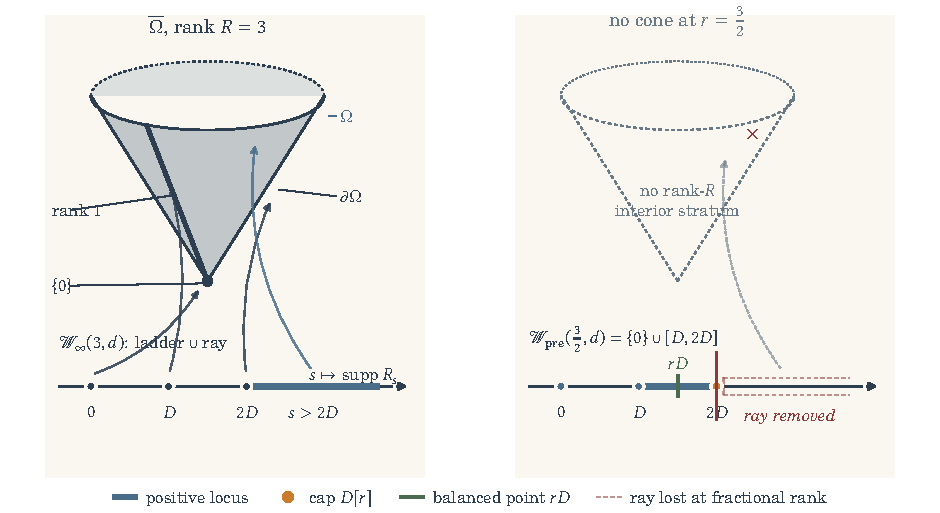
\includegraphics{figs/fig3-cone-strata.pdf}
\caption{The geometric dictionary, and what survives without it. \emph{Left:} at
integer rank $R=3$ the Riesz distribution $R_s$ is a positive measure exactly on
the Wallach set, and at the ladder point $s=jD$ its support is the closure of the
rank-$j$ orbit \cite[Prop.~VII.2.3, Thm.~VII.3.1]{FK}. The map
$s\mapsto\operatorname{supp}R_s$ therefore carries the ladder onto the flag
$\{0\}\subset\overline{\mathcal{O}_1}\subset\partial\Omega$ and carries the
unbounded ray onto the interior $\Omega$; the arrows are that map, and the cone is
a perspective drawing in which only the containment order is meaningful.
\emph{Right:} at $r=\tfrac32$ there is no cone, hence no interior stratum for a
ray to be supported on. What \Cref{thm:band} and \Cref{prop:grid} leave is the
left-hand end of the picture --- the retained grid $\{0,D,2D\}$ and the bounded
band $\mathcal{W}_{\mathrm{pre}}=\{0\}\cup[D,2D]$ containing the balanced point
$rD$, capped at $D\lceil r\rceil$ by \eqref{eq:maxlocus}. The channel to the right
of the cap is where the ray was. The band shown is the pre-erosion locus of
\Cref{thm:band}; at $d=6$ and $d=8$ it subsequently erodes, as
Table~\ref{tab:erosion} records.}
\label{fig:strata}
\end{figure}

\subsection{Spectral and Rank Roots Account for Every Null Mode}
The boundary structure is equally explicit. By \eqref{eq:master-factors} the factor
$s-(i-1)\tfrac{d}{2}+(j-1)$ vanishes when $s=(i-1)\tfrac{d}{2}-k$ with
$0\le k\le\lambda_i-1$, so:

\begin{lemma}[Spectral nulls]
\label{lem:null}
Fix $s$. The monic Jack modes that the spectral factor of \eqref{eq:pivot}
annihilates are exactly
\begin{equation}
  \bigl\{\lambda:F_{\lambda,D}(s)=0\bigr\}
  \;=\;\bigcup_{\substack{i\ge1\\[1pt] k_i:=(i-1)D-s\in\Zint_{\ge0}}}
        \bigl\{\lambda:\lambda_i\ge k_i+1\bigr\},
  \label{eq:nullsupport}
\end{equation}
the union running over every row index $i$ for which the associated $k_i$ is a
nonnegative integer. The nullspace of the pairing at $s$ is spanned by the null
basis modes
\begin{equation}
  \bigl\{\lambda:F_{\lambda,D}(rD)=0\ \text{ or }\ F_{\lambda,D}(s)=0\bigr\},
  \label{eq:nullspace}
\end{equation}
the first alternative being the rank-null ideal of \Cref{lem:ideal} below, which is null
at every $s$. Each null basis mode is a single monic Jack polynomial; arbitrary
linear combinations of null basis modes are again null vectors.
\end{lemma}

A single-cell reading of \eqref{eq:nullsupport} is not correct, for two
reasons. A given numerical value of $s$ may
admit several representations $s=(i-1)D-k$, and the union is over all of them:
at $(\tfrac32,2)$, so $D=1$, the point $s=0$ is both $(3-1)D-2$ and $(1-1)D-0$,
and the mode $\lambda=(1)$ is spectrally null there through the cell $(1,1)$
although $\lambda_3\ge3$ fails. Conversely a mode may be null for the rank
reason rather than the spectral one: at $(\tfrac32,8)$ the mode
$\lambda=(3,3,3)$ is null at $s=12$ because it contains the rank-null cell
$(3,3)$, even though $F_{\lambda,4}(12)=188697600\ne0$ and the representation
$s=(4-1)D-0$ would demand $\lambda_4\ge1$. Only the union
\eqref{eq:nullsupport} together with the ideal describes the nullspace, which is
why \eqref{eq:nullspace} carries both alternatives.

The spectral lattice continues past the classical rank: at $(\tfrac32,8)$ there
are spectral nulls at $s=12,16,20$, contributed by rows $i=4,5,6$ and so
supported on partitions of those lengths. At $(\tfrac32,8)$ and $N=6$ the only
row contributing at $s=7$ is $i=3$, with $k_3=1$, so a spectral null there
requires $\lambda_3\ge2$; the only such partition of size at most $6$ is
$\lambda=(2,2,2)$, and it is not in the rank-null ideal, which needs
$\lambda_3\ge3$.


The rank factor supplies the complementary phenomenon: some partitions are
annihilated identically, at every $s$.

\begin{lemma}[Rank-null partitions]
\label{lem:ideal}
$\Pi_\lambda(r)=0$ if and only if $\lambda$ contains a cell $(i,j)$ with
\begin{equation}
  r+1-i+\alpha(j-1)=0.
  \label{eq:idealcell}
\end{equation}
The partitions containing such a cell form an ideal in the containment order,
and they drop out of the pairing at every $s$.
\end{lemma}

In the defect variable \eqref{eq:rankcell} the condition \eqref{eq:idealcell} on
the first sub-diagonal row $i=\lceil r\rceil+1$ (that is $t=0$) reads $j-1=\nu$,
so an ideal cell on the first sub-diagonal exists precisely when the defect is a
positive integer:
\begin{equation}
  \nu\in\Zint_{>0}\;\Longrightarrow\;\text{ideal cell }
  \bigl(\lceil r\rceil+1,\;\nu+1\bigr).
  \label{eq:idealnu}
\end{equation}
At integer rank $\nu=0$ and the cell is $(\lceil r\rceil+1,1)$, recovering the
familiar length ideal $\lambda_{\lceil r\rceil+1}\ge1$, equivalently
$\ell(\lambda)>\lceil r\rceil$, used in \Cref{thm:intrank}.

\Needspace*{14\baselineskip}
\subsection{The Content Set Generates a Principal Rank-Null Ideal}
The first sub-diagonal is not the whole story, and the content set settles the
rest of it exactly. By \eqref{eq:pivot} a cell $(i,j)$ is rank-null precisely
when $rD=(i-1)D-(j-1)$, so the question is whether the rescaled rank meets
$\Lambda_D$, and if it does, which cells realize it.

\begin{proposition}{The content set generates a principal rank-null ideal}{idealfull}
Let $D>0$ and $r\in\Rr$. A rank-null cell exists if and only if
$rD\in\Lambda_D$; for $D=a/b$ in lowest terms this says $ar\in\Zint$, and for
irrational $D$ at most one such cell can exist. If none exists, no partition is
rank-null. If one exists, let $(i_0,j_0)$ be the coordinatewise minimal solution
of
\begin{equation}
  rD\;=\;(i_0-1)D-(j_0-1),\qquad i_0,j_0\in\Zint_{\ge1}.
  \label{eq:idealmin}
\end{equation}
For rational $D=a/b$ the rank-null cells are then exactly
\begin{equation}
  (i_0+tb,\;j_0+ta),\qquad t\in\Zint_{\ge0},
  \label{eq:idealprog}
\end{equation}
and in every case the rank-null partitions form the single principal ideal
\begin{equation}
  \bigl\{\lambda:\Pi_\lambda(r)=0\bigr\}\;=\;\bigl\{\lambda:\lambda_{i_0}\ge j_0\bigr\},
  \label{eq:idealprincipal}
\end{equation}
generated by the rectangle $(j_0^{\,i_0})$ and therefore first active at degree
$i_0j_0$.
\end{proposition}

\begin{proof}[Proof of \Cref{prop:idealfull}]
Writing $p=i-1$ and $q=j-1$, the vanishing condition is $pD-q=rD$ with
$p,q\in\Zint_{\ge0}$, and its right-hand side runs over $\Lambda_D$ as $(i,j)$
runs over $\Zint_{\ge1}^{2}$; this is the existence criterion. If $D$ is
irrational then $pD-q=p'D-q'$ forces $p=p'$ and $q=q'$, so a solution is unique.
If $D=a/b$ in lowest terms the equation reads $pa-qb=ra$, so $ra\in\Zint$ is
necessary; it is sufficient because $\gcd(a,b)=1$ makes $pa-qb=m$ solvable in
integers for every $m\in\Zint$, and replacing $(p,q)$ by $(p+tb,q+ta)$ preserves
$pa-qb$, so some shift has both coordinates nonnegative. The same shift accounts
for all solutions, again by $\gcd(a,b)=1$, and both coordinates increase with
$t$; hence the nonnegative solutions are the shifts by $t\ge0$ of the
coordinatewise minimal one, which is \eqref{eq:idealprog}.

For \eqref{eq:idealprincipal}, a partition with $\lambda_{i_0}\ge j_0$ contains
$(i_0,j_0)$ and is rank-null. Conversely, if $\lambda$ contains a rank-null cell
$(i_0+tb,j_0+ta)$ with $t\ge0$ then $\lambda_{i_0}\ge\lambda_{i_0+tb}\ge
j_0+ta\ge j_0$, since $\lambda$ is nonincreasing; in the irrational case $t=0$ is
the only option and the implication is immediate. The ideal is therefore
generated by the single rectangle $(j_0^{\,i_0})$.
\end{proof}

In the defect variable the existence criterion and the minimal cell take a form
that makes the later-row case routine. Writing $D=a/b$ in lowest terms and
$k=\lceil r\rceil$, one has $ar=ak-b\nu$, so \Cref{prop:idealfull} becomes a
statement about $b\nu$.

\begin{corollary}[Defect form of the rank-null criterion]
\label{cor:defectideal}
Let $r>0$, let $D=a/b$ in lowest terms, put $k=\lceil r\rceil$ and
$\nu=D(k-r)$. A rank-null cell exists if and only if $b\nu\in\Zint$, giving the
trichotomy
\begin{enumerate}
\item[(i)] $b\nu\notin\Zint$: no rank-null ideal, at any degree or row;
\item[(ii)] $\nu\in\Zint_{\ge0}$: the minimal null cell lies in row
  $k+1$, namely $(k+1,\nu+1)$;
\item[(iii)] $b\nu\in\Zint$ but $\nu\notin\Zint$: the minimal null cell lies in a
  strictly later row.
\end{enumerate}
In cases (ii) and (iii), put $m=b\nu\in\Zint_{\ge0}$ and let
$t_0\in\{0,\dots,b-1\}$ be the least solution of $m+at_0\equiv0\pmod b$. Then the
minimal rank-null cell is
\begin{equation}
  \Bigl(k+1+t_0,\ 1+\tfrac{m+at_0}{b}\Bigr),
  \label{eq:mincell}
\end{equation}
and the rank-null partitions form the principal ideal it generates.
\end{corollary}

\begin{proof}[Proof of \Cref{cor:defectideal}]
From $rD=kD-\nu$ and $D=a/b$, $ar=ak-b\nu$, so $ar\in\Zint$ if and only if
$b\nu\in\Zint$; this is the existence criterion of \Cref{prop:idealfull}. When
$\nu\in\Zint_{\ge0}$ the cell $(k+1,\nu+1)$ is rank-null by \eqref{eq:idealnu}
and is minimal, giving (ii); at $\nu=0$ this is the integer-rank length ideal
generated by $(k+1,1)$, with $k=r$, and \eqref{eq:mincell} returns it because
$m=t_0=0$; when $b\nu\in\Zint$ but $\nu\notin\Zint$ no first-row cell
$(k+1,\nu+1)$ is integral, so the minimal cell has $t_0\ge1$, giving (iii). For
\eqref{eq:mincell}, the rank-null condition $(i-1)D-(j-1)=rD$ with $i=k+1+t$ reads
$tD-(j-1)=-\nu$, i.e.\ $b(j-1)=m+at$; the least $t\ge0$ making the right side
divisible by $b$ is $t_0$, and then $j-1=(m+at_0)/b$. Minimality and the
principal-ideal statement are \Cref{prop:idealfull}.
\end{proof}

The scattered examples now read off \eqref{eq:mincell} uniformly. At
$(\tfrac32,8)$, $D=4$ so $a=4,b=1$ and $b\nu=2$: case (ii), minimal cell $(3,3)$,
ideal $\lambda_3\ge3$ generated by $(3,3,3)$, first active at $N=9$. At
$(\tfrac52,8)$, $b\nu=2$ again, minimal cell $(4,3)$. At $(\tfrac23,3)$,
$D=\tfrac32$ so $a=3,b=2$ and $\nu=\tfrac12$, $b\nu=1\in\Zint$ while
$\nu\notin\Zint$: case (iii), $t_0=1$, minimal cell $(3,3)$ on the second
sub-diagonal. By contrast $(\tfrac32,2)$, $(\tfrac32,6)$, $(\tfrac32,10)$ and
$(\tfrac32,3)$ give $b\nu=\tfrac12,\tfrac32,\tfrac52,\tfrac32$, none integral:
case (i), no rank-null partition at any degree or row.


\subsection{Defect Arithmetic Decides Whether the Upper Edge Erodes}
Upper-edge erosion is governed by the lattice of cells below row
$\lceil r\rceil$. Rectangular partitions often provide the first witness, but no
single cell controls the general case.

\begin{lemma}[Upper-edge sign rule]
\label{lem:upper}
Let $r>0$ be real with $r\notin\Zint$, put $k=\lceil r\rceil$, and write
$s=kD-\varepsilon$. For a cell $c=(i,j)$ with $i=k+1+t$, $t\ge0$, set
$u(c)=j-1-tD$; then the rank factor of $c$ is $(u(c)-\nu)/D$ and its spectral
factor is $u(c)-\varepsilon$. For $0<\varepsilon<D$, cells in rows $i\le k$
contribute positive factors to both.

Fix a partition $\lambda$, and suppose in addition that $\varepsilon$ is smaller
than every positive value $u(c)$ occurring in $\lambda$. Then,
uniformly over the cells of that diagram, $c$ contributes a sign disagreement
exactly when
\begin{equation}
  0\;<\;j-1-tD\;<\;\nu,
  \label{eq:upperlattice}
\end{equation}
and $c$ is rank-null exactly when $j-1-tD=\nu$.
\end{lemma}

\begin{proof}[Proof of \Cref{lem:upper}]
The rank factor is $\bigl((j-1)-\nu-tD\bigr)/D=(u(c)-\nu)/D$ by
\eqref{eq:rankcell}, and the spectral factor is
$s-(i-1)D+(j-1)=u(c)-\varepsilon$. For a cell in a row $i\le k$ both factors are
positive once $\varepsilon<D$: the smallest spectral factor is that of $(k,1)$,
namely $D-\varepsilon$, and the rank factors are those of \Cref{thm:band}. Take
$\varepsilon$ smaller than $D$ and than every positive value $u(c)$ occurring in
$\lambda$ --- finitely many conditions, so some $\varepsilon>0$ meets them all,
and one such $\varepsilon$ serves every cell of $\lambda$ at once. Then
$\operatorname{sign}(u(c)-\varepsilon)=\operatorname{sign}(u(c))$ whenever
$u(c)\ne0$, while $u(c)=0$ makes both factors negative. The signs of
$u(c)-\nu$ and $u(c)$ differ precisely when $0<u(c)<\nu$.
\end{proof}

\begin{theorem}{A lattice-gap criterion protecting the upper edge}{erosion}
Let $r>0$ be real with $r\notin\Zint$, put $k=\lceil r\rceil$, and suppose
\begin{equation}
  \bigl(tD,\;tD+\nu\bigr)\cap\Zint=\varnothing
  \qquad\text{for every } t\in\Zint_{\ge0}.
  \label{eq:nolattice}
\end{equation}
Then, for every cutoff $N$,
\begin{equation}
  [\,rD,\;kD\,]\;\subseteq\;\mathcal{W}_N(r,d),
  \label{eq:upperband}
\end{equation}
and consequently
\begin{equation}
  [\,rD,\;kD\,]\;\subseteq\;\mathcal{W}_\infty(r,d).
  \label{eq:upperbandinf}
\end{equation}
Every pivot is nonnegative throughout $rD\le s\le kD$, and every pivot outside
the rank-null ideal is strictly positive for $rD<s<kD$. If $D=a/b$ in lowest
terms, then \eqref{eq:nolattice} holds if and only if
\begin{equation}
  \nu\;\le\;\frac1b ,
  \label{eq:nub}
\end{equation}
and if $D$ is irrational then \eqref{eq:nolattice} fails for every $\nu>0$. In
particular, for $D\in\Zint_{>0}$, equivalently $d\in2\Zint_{>0}$:
\begin{enumerate}
\item[(i)] if $\nu<1$ the upper half-band is strictly positive away from the
  rank-null ideal;
\item[(ii)] if $\nu=1$ the critical rectangle $(2^{\,k+1})$ lies in the
  rank-null ideal and the upper edge remains stable;
\item[(iii)] if $\nu>1$ the upper edge erodes, $(2^{\,k+1})$ giving a negative
  pivot immediately below $s=kD$.
\end{enumerate}
\end{theorem}

\begin{proof}[Proof of \Cref{thm:erosion}]
Write $s=kD-\varepsilon$ with $0\le\varepsilon\le\nu$, which is exactly the range
$rD\le s\le kD$. For a cell in a row $i\le k$ the rank factor is positive, its
least value being $r-k+1=1-\nu/D>0$ at $(k,1)$, and its spectral factor is
positive as well, since $s-(i-1)D+(j-1)\ge s-(k-1)D=D-\varepsilon\ge D-\nu>0$.

For a cell in row $i=k+1+t$ with $t\ge0$ put $u=j-1-tD$, so by \Cref{lem:upper}
the rank factor is $(u-\nu)/D$ and the spectral factor is $u-\varepsilon$.
Condition \eqref{eq:nolattice} says precisely that no attainable $u$ lies in the
open interval $(0,\nu)$, so either $u\le0$ or $u\ge\nu$. If $u\le0$ then
$u-\nu<0$ and $u-\varepsilon\le0$; if $u\ge\nu$ then $u-\nu\ge0$ and
$u-\varepsilon\ge u-\nu\ge0$. In both cases the two factors carry the same weak
sign, so every pivot is nonnegative on $[rD,kD]$. For $0<\varepsilon<\nu$ a
vanishing factor requires $u=\nu$, which is the rank-null condition, so every
pivot outside the rank-null ideal is strictly positive on the open interval.

For \eqref{eq:nub}, write $D=a/b$ in lowest terms. The fractional parts of $tD$
run through $0,\tfrac1b,\dots,\tfrac{b-1}{b}$, so the least positive distance
from a point $tD$ up to the next integer is $\tfrac1b$. Since the interval in
\eqref{eq:nolattice} is open, it avoids $\Zint$ for every $t$ exactly when
$\nu\le\tfrac1b$. If $D$ is irrational the fractional parts of $tD$ are dense
modulo $1$, so those distances are arbitrarily small and \eqref{eq:nolattice}
fails for every $\nu>0$.

Finally let $D\in\Zint_{>0}$, so $b=1$ and stability holds exactly when
$\nu\le1$. If $\nu=1$ the cell $(k+1,2)$ has $u=1=\nu$ and is rank-null. If
$\nu>1$, take $\lambda=(2^{\,k+1})$. Its bottom row has normalized rank factors
$-\nu/D$ and $(1-\nu)/D$, both negative, so an even number; immediately below $kD$ its
spectral factors are $-\varepsilon$ and $1-\varepsilon$, exactly one negative.
All cells in the first $k$ rows contribute positively, so
$\pi_\lambda(kD-\varepsilon)<0$ for all small $\varepsilon>0$.
\end{proof}

Condition \eqref{eq:nolattice} is sufficient but not necessary. The sign rule of
\Cref{lem:upper} decides the question exactly, and it is worth stating separately,
because the erosion census of the next subsection is read against it rather than
against \eqref{eq:nolattice}.

\begin{proposition}{Exact upper-edge erosion criterion}{erosionexact}
Let $r>0$ be real with $r\notin\Zint$, put $k=\lceil r\rceil$, and set
\begin{equation}
  \mathcal{M}=\bigl\{(k+1+t,j):0<j-1-tD<\nu\bigr\},
  \qquad
  \mathcal{Z}=\bigl\{(k+1+t,j):j-1-tD=\nu\bigr\}.
  \label{eq:MZ}
\end{equation}
For a fixed $\lambda$ and all sufficiently small $\varepsilon>0$: if
$\lambda\cap\mathcal{Z}\ne\varnothing$ then $\pi_\lambda(kD-\varepsilon)=0$, and
if $\lambda\cap\mathcal{Z}=\varnothing$ then
$\operatorname{sign}\pi_\lambda(kD-\varepsilon)=(-1)^{|\lambda\cap\mathcal{M}|}$.
Consequently the upper edge erodes if and only if some finite diagram $\lambda$
satisfies
\begin{equation}
  \lambda\cap\mathcal{Z}=\varnothing
  \qquad\text{and}\qquad
  |\lambda\cap\mathcal{M}|\equiv1\!\!\pmod 2 .
  \label{eq:erosionexact}
\end{equation}
\end{proposition}

\begin{proof}[Proof of \Cref{prop:erosionexact}]
By \Cref{lem:upper} a cell $c$ of $\lambda$ contributes a sign disagreement
exactly when $c\in\mathcal{M}$, and contributes a vanishing rank factor exactly
when $c\in\mathcal{Z}$; all other cells contribute agreeing nonzero signs. A
product is zero as soon as one factor is, and otherwise its sign is the parity of
the number of disagreements, which is \eqref{eq:erosionexact}. The upper edge
erodes precisely when some pivot is strictly negative immediately below $kD$.
\end{proof}

Condition \eqref{eq:nolattice} is the special case $\mathcal{M}=\varnothing$, and
the integer-step trichotomy above is the corollary of
\Cref{prop:erosionexact} at $b=1$. The gap between the two is real: at
$r=\tfrac43$, $d=3$ one has $D=\tfrac32$ and $\nu=1$, so
$\mathcal{M}\ne\varnothing$ and \eqref{eq:nolattice} fails, yet every diagram
reaching a cell of $\mathcal{M}$ also meets $\mathcal{Z}$ and is annihilated, so
the edge does not erode.

The hypothesis $D\in\Zint$ in the second half is not decorative. When $D$ is not
an integer the lattice condition \eqref{eq:nolattice} can fail at some $t\ge1$
even though $\nu<1$, and then the upper edge erodes at a degree well above
$2(k+1)$.

\subsection{The Census Reveals Protected, One-Sided, and Two-Sided Erosion}
\label{sec:census}

With the mechanism in hand the computed loci can be read as a census. Three
examples separate the possibilities --- a small defect that fails to protect the
edge, erosion from below, and an ideal that halts erosion after one step --- and
the figure and table then display the whole phenomenology at once.

\begin{remark}[A small defect does not protect the upper edge]
\label{rem:latticewitness}
Take $r=\tfrac32$ and $d=3$, so $D=\tfrac32$, $k=2$ and $\nu=\tfrac34<1$.
Condition \eqref{eq:nolattice} holds at $t=0$, but at $t=1$ the interval
$\bigl(\tfrac32,\tfrac94\bigr)$ contains the integer $2$, and the cell with
$t=1$, $j=3$ has $u=\tfrac12\in(0,\nu)$. The rectangle
$\lambda=(3,3,3,3)$ realizes exactly one such cell. Its rank factor
$F_{\lambda,3/2}(\tfrac94)$ is a positive rational (the exact value is emitted by
\texttt{ancillary\_census.py}), while its spectral factor $F_{\lambda,3/2}(s)$ is negative for
$\tfrac52<s<3$, so $\pi_\lambda(s)<0$ there. The upper edge therefore erodes at
degree $12$: the locus is $\{0,\tfrac32\}\cup[2,3]$ at $N=6$ and
$\{0,\tfrac32\}\cup[2,\tfrac52]\cup\{3\}$ at $N=12$. Every fractional row of
Table~\ref{tab:erosion} and Figure~\ref{fig:loci} has $d$ even, hence
$D\in\Zint$, so those rows are governed by the trichotomy above; the phenomenon
here is invisible at even $d$.
\end{remark}

The threshold is not monotone in $d$: at $\nu=1$ the cell
that would produce a negative pivot is the same cell that annihilates the
partition, so $\nu=1$ is protected for a different reason than $\nu<1$. The
governing quantity is therefore the defect together with the arithmetic of $D$,
not the multiplicity by itself; \texttt{ancillary\_census.py} records pairs on
either side of the threshold at each of $d<4$ and $d>4$, including a case with
$\nu<1$ that erodes because $D\notin\Zint$.

\Cref{thm:erosion} concerns the upper edge alone. It does not assert that the
band is stable, and in general the band can also erode from below. The exact
witness is
\begin{equation}
  r=\tfrac32,\quad d=3,\quad \nu=\tfrac34,\quad s=\tfrac{13}{8},
  \quad \lambda=(2,2,2),
  \label{eq:belowwitness}
\end{equation}
for which $F_{\lambda,D}(rD)<0$ and $F_{\lambda,D}(s)>0$, so the pivot is
strictly negative at a point interior to the band $[\tfrac32,3]$ predicted by
\Cref{thm:band}, near its lower endpoint. The computed locus changes from
$\{0\}\cup[\tfrac32,3]$ at $N=5$ to $\{0,\tfrac32\}\cup[2,3]$ at $N=6$: the lower
endpoint has increased while the upper endpoint is intact. Statements about
stability of the whole band therefore require a separate argument, such as
\Cref{thm:d2} at $d=2$.

At $(\tfrac32,8)$ the critical rectangle is $\lambda=(2,2,2)$, with
$\operatorname{sign}\Pi_\lambda(\tfrac32)=+1$ and
\begin{equation}
  (s)^{(1/4)}_{(2,2,2)}\;=\;s\,(s+1)(s-3)(s-4)(s-7)(s-8),
  \label{eq:pivot222}
\end{equation}
a sextic that is negative on $(-1,0)\cup(3,4)\cup(7,8)$ and, within the band
$[4,8]$, negative exactly on the open cell $(7,8)$. At cutoff $N=6$ the Gram form
acquires exactly one negative direction throughout $7<s<8$, and at $s=7$ its
unique null mode is $P_{(2,2,2)}$ --- \texttt{ancillary\_census.py} records the
full inertia of that cutoff. The band's upper boundary
drops from $8$ to $7$, and $s=8$ survives in isolation. Every deeper erosion candidate at $(\tfrac32,8)$
--- the Pochhammer zeros at $s=6$ and $s=5$ inside the band --- requires
$\lambda_3\ge3$ and therefore lies in the rank-null ideal. This is the cellwise
argument behind the stability observed below; it is the ideal, not the size of
the cutoff, that ends the erosion.

\begin{figure}[htbp]
\centering
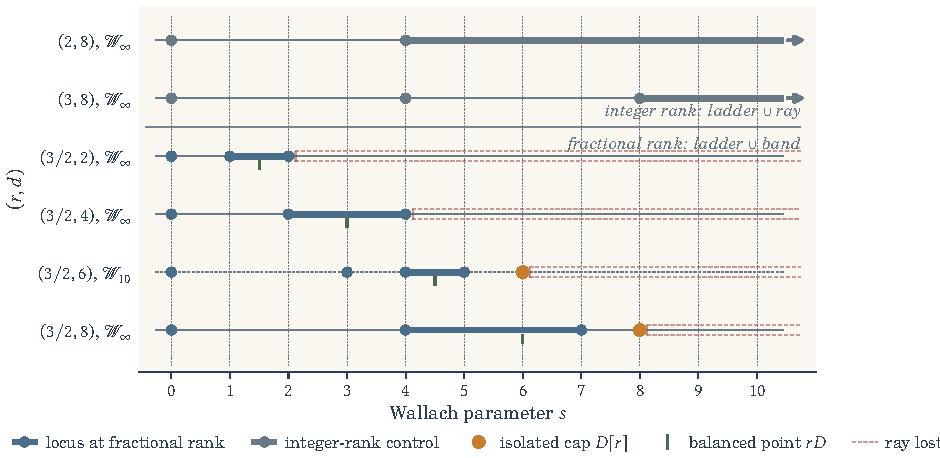
\includegraphics{figs/fig4-positivity-loci.pdf}
\caption{Positivity at integer and fractional rank; each row is labelled with the
locus it shows, and the one finite-cutoff row carries a dashed rule. The grey
integer controls ($r=2,3$), governed by \Cref{thm:intrank}, carry the classical
ladder and an unbounded ray. Every fractional row has $r=\tfrac32$, and its ray is
replaced by a bounded band whose erosion is decided by the defect
$\nu=\tfrac{d}{4}$: none at $d=2,4$, one step at $d=8$ before the rank-null ideal
halts it, two-sided at $d=6$, where no ideal exists. An amber mark is an isolated
cap point $D\lceil r\rceil$, retained at every degree by \Cref{prop:grid} and
maximal in its locus by \eqref{eq:maxlocus}; the short rule beneath each
fractional row is the balanced point $rD$ of \eqref{eq:balanced}, which every
band contains. All loci are exact. Every
fractional row has $d$ even, so \Cref{thm:erosion}(i)--(iii) applies; see
\Cref{rem:latticewitness} for odd $d$.}
\label{fig:loci}
\end{figure}

Table~\ref{tab:erosion} records the exact loci. Each entry is an algebraic cell
decomposition in exact rational arithmetic at the stated cutoff.

\begin{table}[htbp]
\centering
\caption{Exact positivity loci at selected fractional ranks. Every row has even
$d$, so $D\in\Zint$, and erosion is governed by the defect
$\nu=D(\lceil r\rceil-r)$ rather than by $d$. The row $(\tfrac32,2)$, with
$\nu=\tfrac12$, never moves, by \Cref{thm:d2}. The row $(\tfrac32,4)$, with
$\nu=1$, is stable from $N_*=3$ on, by \Cref{thm:stab} and \Cref{thm:ncut}. The
two rows with $\nu=2$ erode once, at $N=2(\lceil r\rceil+1)$, and are then
stopped by the rank-null ideal. The row $(\tfrac32,6)$, whose $\nu=\tfrac32$
admits no ideal, erodes twice, at $N=6$ and again at $N=9$.}
\label{tab:erosion}
\smallskip
\small
\begin{tabular}{@{}l l l l @{}}
\toprule
\estabhead{$(r,d)$} & \estabhead{$N=4$} & \estabhead{$N=6$} & \estabhead{$N=8$}\\
\midrule
$(\tfrac32,2)$ & $\{0\}\cup[1,2]$ & $\{0\}\cup[1,2]$ & $\{0\}\cup[1,2]$\\
$(\tfrac32,4)$ & $\{0\}\cup[2,4]$ & $\{0\}\cup[2,4]$ & $\{0\}\cup[2,4]$\\
$(\tfrac32,6)$ & $\{0\}\cup[3,6]$ & $\{0\}\cup[3,5]\cup\{6\}$ & $\{0\}\cup[3,5]\cup\{6\}$\\
$(\tfrac32,8)$ & $\{0\}\cup[4,8]$ & $\{0\}\cup[4,7]\cup\{8\}$ & $\{0\}\cup[4,7]\cup\{8\}$\\
$(\tfrac52,8)$ & $\{0,4\}\cup[8,12]$ & $\{0,4\}\cup[8,12]$ & $\{0,4\}\cup[8,11]\cup\{12\}$\\
\bottomrule
\end{tabular}

\smallskip

\begin{tabular}{@{}l l l @{}}
\toprule
\estabhead{$(r,d)$} & \estabhead{$N=9$} & \estabhead{$N=10$}\\
\midrule
$(\tfrac32,2)$ & $\{0\}\cup[1,2]$ & $\{0\}\cup[1,2]$\\
$(\tfrac32,4)$ & $\{0\}\cup[2,4]$ & $\{0\}\cup[2,4]$\\
$(\tfrac32,6)$ & $\{0\}\cup\{3\}\cup[4,5]\cup\{6\}$ & $\{0\}\cup\{3\}\cup[4,5]\cup\{6\}$\\
$(\tfrac32,8)$ & $\{0\}\cup[4,7]\cup\{8\}$ & $\{0\}\cup[4,7]\cup\{8\}$\\
$(\tfrac52,8)$ & $\{0,4\}\cup[8,11]\cup\{12\}$ & $\{0,4\}\cup[8,11]\cup\{12\}$\\
\bottomrule
\end{tabular}
\end{table}

\FloatBarrier

\section{Arithmetic Controls the Surviving Locus and Its Stabilization}
\label{sec:arith}

Arithmetic now separates three regimes, and it is worth having the whole map
before the casework begins. Write $D=a/b$ in lowest terms and
$\nu=D(\lceil r\rceil-r)$. \Cref{cor:defectideal} sorts every positive rank into
exactly one of three classes according to the arithmetic of $b\nu$, and the class
determines both which rank-null ideal exists and which stabilization mechanism is
available.

\begin{center}
\footnotesize
\begin{tabular}{@{}l l l@{}}
\toprule
\estabhead{condition} & \estabhead{rank-null ideal}
  & \estabhead{known stabilization mechanism}\\
\midrule
$b\nu\notin\Zint$ & none, at any row
  & finite rational sign stratification\\
$b\nu\in\Zint$, $\nu\notin\Zint$ & later-row principal ideal
  & ideal together with finite stratification\\
$\nu\in\Zint_{>0}$ & first-subdiagonal ideal
  & exact falling-factorial staircase\\
\bottomrule
\end{tabular}
\captionof{table}{The arithmetic regimes at positive nonintegral rank, and what
is known in each. The three conditions are exhaustive and mutually exclusive.
Effectivity is available only in the third row and in the unit-numerator case
$a=1$ of the first; \Cref{thm:ratstab} supplies stabilization without a threshold
throughout.}
\label{tab:regimes}
\end{center}

\medskip
\noindent
When the numerator of $D$ is one, the cell chamber fills the whole initial band
and no erosion occurs, so the locus can be written down completely. At integral
defect the surviving locus follows an exact falling-factorial staircase and
stabilizes at a computable degree. Outside these two regimes the band may
fragment; stabilization still occurs at every rational step, but no uniform
stable-locus formula is presently known.

\subsection{Unit-Numerator Steps Prevent Erosion}

At $d=2$ the content set is $\Zint$, the chamber containing $rD=r$ is
$[\lfloor r\rfloor,\lfloor r\rfloor+1]$, and the whole locus can be written down
at every positive nonintegral rank.

\begin{theorem}{Unit cell step prevents erosion}{d2}
Let $r>0$ be nonintegral and write $m=\lfloor r\rfloor$. Then
\begin{equation}
  \mathcal{W}_\infty(r,2)
  \;=\;\{0,1,\dots,m-1\}\;\cup\;[m,\,m+1],
  \label{eq:d2locus}
\end{equation}
the finite set being empty when $m=0$, and the pairing is positive definite
throughout $m<s<m+1$.
\end{theorem}

\begin{proof}[Proof of \Cref{thm:d2}]
Here $D=1$, so a cell $(i,j)$ contributes $r+j-i$ to the rank factor and $s+j-i$
to the spectral factor; both depend on the cell only through the integer $m'=j-i$.

If $m<s<m+1$ then $r$ and $s$ lie in the same component of $\Rr\setminus\Zint$,
so for every integer $m'$ the numbers $r+m'$ and $s+m'$ do too, and in particular
share a nonzero sign. By \eqref{eq:interlock} every pivot is strictly positive,
and the argument is cellwise, hence independent of the degree. This is
\Cref{thm:chamber} for $\Lambda_1=\Zint$. At the endpoints $s=m$ and $s=m+1$ the
same comparison gives weakly matching signs, with spectral zeros permitted, so
the closed band lies in $\mathcal{W}_\infty(r,2)$.

The ladder points $0,1,\dots,m-1$ are retained exactly as in
\Cref{thm:intrank}: at $s=j<m$ a partition with at most $j$ rows has strictly
positive spectral factors, and one with more contains the cell $(j+1,1)$, whose
spectral factor vanishes. The gaps $(j,j+1)$ with $0\le j\le m-1$ are excluded by
the column $(1^{\,j+2})$, which has exactly one negative spectral factor and no
negative rank factor; $s<0$ is excluded by the one-box partition $\lambda=(1)$; and $s>m+1$ is excluded by
\Cref{prop:cap}, whose witness is the column $(1^{\,m+2})$. These exhaust $\Rr$.
\end{proof}

The same argument runs verbatim whenever the initial band is a single cell
chamber, which happens exactly when $D$ has numerator $1$.

\Needspace*{9\baselineskip}
\begin{boxedcorollary}{Unit-numerator steps}{unitstep}
Let $b\in\Zint_{>0}$ and $d=2/b$, so $D=1/b$. Then for every positive nonintegral
$r$,
\begin{equation}
  \mathcal{W}_\infty(r,2/b)
  =\Bigl\{\tfrac jb:0\le j<\lfloor r\rfloor\Bigr\}
  \;\cup\;\Bigl[\tfrac{\lfloor r\rfloor}{b},\;\tfrac{\lceil r\rceil}{b}\Bigr].
  \label{eq:unitstep}
\end{equation}
\end{boxedcorollary}

\begin{proof}[Proof of \Cref{bcor:unitstep}]
With $D=1/b$ in lowest terms, $\Lambda_D=b^{-1}\Zint$ by \Cref{thm:chamber}, and
$rD=r/b$ lies in the interior of the chamber
$[\lfloor r\rfloor/b,\lceil r\rceil/b]$ because $r$ is not an integer. That
chamber is exactly the initial band $[\lfloor r\rfloor D,\lceil r\rceil D]$ of
\Cref{thm:band}, so \Cref{thm:chamber} places all of it in
$\mathcal{W}_\infty$, at every degree. The ladder points, the gaps below, the
negative axis and the region above $\lceil r\rceil D$ are handled exactly as in
\Cref{thm:d2} and \Cref{prop:cap}.
\end{proof}

Thus $N_{\mathrm{er}}=\infty$ whenever the numerator of $D$ is $1$, and no
erosion occurs at any degree. Erosion is possible only when the initial band
strictly contains a cell chamber: among rational steps, exactly when $D$ has
numerator at least $2$. For irrational $D$ the content set is dense and no
nondegenerate chamber exists at all.

\subsection{Integral Defect Leaves One Interval and Finitely Many Isolated Points}

When the defect is a positive integer, the entire integral-defect
classification --- the exact locus at each cutoff, the all-degree locus, the
stabilization degree, and every erosion event --- follows from one
one-dimensional identity. On the terminal chamber the pivot is a product of two
falling factorials, and the whole sign analysis reduces to reading their signs.

Throughout this subsection $k=\lceil r\rceil$ and $\nu=D(k-r)\in\Zint_{>0}$, so $0<\nu<D$ and
$rD=kD-\nu$; by \eqref{eq:idealnu} the rank-null ideal is
$\lambda_{k+1}\ge\nu+1$. Write $x^{\underline m}=x(x-1)\cdots(x-m+1)$ for the
falling factorial, with the empty product read as $1$.

\begin{lemma}[Terminal falling-factorial reduction]
\label{lem:terminal}
Let $\lambda$ lie outside the rank-null ideal, put $m=\lambda_{k+1}\le\nu$, and
write $s=kD-\sigma$ with $0\le\sigma\le D$. Then
\begin{equation}
  \pi_\lambda(kD-\sigma)\;=\;C_\lambda(\sigma)\,\nu^{\underline m}\,
  \sigma^{\underline m},
  \label{eq:terminalpivot}
\end{equation}
where $C_\lambda(\sigma)>0$ for $0\le\sigma<D$ and $C_\lambda(D)\ge0$.
Consequently, on the interior $0\le\sigma<D$ the sign of the pivot is exactly the
sign of $\sigma^{\underline m}$.
\end{lemma}

\begin{proof}[Proof of \Cref{lem:terminal}]
By \eqref{eq:pivot} the pivot is $D^{-|\lambda|}H_\lambda(D)^{-1}$ times the
product over cells of the rank factor $D(r-i+1)+(j-1)$ and the spectral factor
$s-(i-1)D+(j-1)$; the scalar is positive, so it is absorbed into $C_\lambda$ and
we track the two cell products. For a cell in a row $i\le k$ both factors are
positive when $0\le\sigma<D$: their least values are $r-k+1=1-\nu/D>0$ and
$s-(k-1)D=D-\sigma>0$. At $\sigma=D$ the spectral factors are still nonnegative.

For a cell in row $i=k+1+t$ write $q=j-1$. The rank factor is $q-\nu-tD$ and the
spectral factor is $q-\sigma-tD$. Because $\lambda$ lies outside the ideal,
$q\le\lambda_{k+1}-1=m-1\le\nu-1$. For $t\ge1$ both factors are strictly
negative, since $q\le\nu-1<\nu\le tD\le\sigma+tD$ and $q<\nu<D\le tD$; their
product is positive and contributes to $C_\lambda$. The remaining cells, in row
$t=0$, contribute
\begin{equation*}
  \prod_{q=0}^{m-1}(q-\nu)(q-\sigma)
  \;=\;\prod_{q=0}^{m-1}(\nu-q)(\sigma-q)
  \;=\;\nu^{\underline m}\,\sigma^{\underline m}.
\end{equation*}
Collecting, $\pi_\lambda(kD-\sigma)=C_\lambda(\sigma)\,\nu^{\underline m}
\sigma^{\underline m}$ with $C_\lambda$ a product of positive factors for
$0\le\sigma<D$, hence positive there, and nonnegative at $\sigma=D$. Since
$\nu^{\underline m}>0$ for $m\le\nu$, the interior sign is that of
$\sigma^{\underline m}$.
\end{proof}

The one-dimensional problem is now transparent. At cutoff $N$ the terminal
chamber is tested by exactly those falling factorials $\sigma^{\underline m}$
whose rectangle $(m^{\,k+1})$ fits, that is $1\le m\le M_N$. Their common
nonnegativity set is an elementary interval-plus-points, and the statement
involves no parameter of the pairing: the mechanism is simply that a nonintegral
$\sigma\ge0$ has its first negative falling factorial at order
$\lfloor\sigma\rfloor+2$, while an integral $\sigma\ge0$ reaches zero there
instead and stays zero.

\begin{lemma}[Common nonnegativity of initial falling factorials]
\label{lem:onevar}
For every integer $M\ge1$,
\begin{equation}
  \bigl\{\sigma\in\Rr:\sigma^{\underline m}\ge0\ \text{for every }1\le m\le M\bigr\}
  \;=\;\{0,1,\dots,M-2\}\;\cup\;[M-1,\,\infty),
  \label{eq:onevar}
\end{equation}
the finite set being empty when $M=1$.
\end{lemma}

\begin{proof}[Proof of \Cref{lem:onevar}]
If $\sigma\ge M-1$ then $\sigma\ge m-1$ for every $m\le M$, so every factor of
$\sigma^{\underline m}=\sigma(\sigma-1)\cdots(\sigma-m+1)$ is nonnegative. If
$\sigma=n\in\{0,\dots,M-2\}$ then $\sigma^{\underline m}$ is a product of
positive factors for $m\le n$ and vanishes for every $m\ge n+1$. Every remaining
$\sigma$ is either negative, in which case $\sigma^{\underline1}<0$, or satisfies
$n<\sigma<n+1$ for some $0\le n\le M-2$, in which case $\sigma^{\underline{n+2}}$
has exactly one negative factor, namely $\sigma-(n+1)$, and $n+2\le M$, so the
offending constraint is present.
\end{proof}

\begin{theorem}{The exact finite-cutoff erosion staircase}{staircase}
Let $r>0$, $r\notin\Zint$, with $\nu=D(\lceil r\rceil-r)\in\Zint_{>0}$, put
$k=\lceil r\rceil$, and for $N\ge k+1$ set
\begin{equation}
  M_N\;=\;\min\!\Bigl(\nu,\ \bigl\lfloor\tfrac{N}{k+1}\bigr\rfloor\Bigr).
  \label{eq:MN}
\end{equation}
Then the exact cutoff-$N$ positivity locus is
\begin{equation}
  \mathcal{W}_N(r,d)
  \;=\;\bigl\{jD:0\le j\le k-2\bigr\}
  \;\cup\;[(k-1)D,\;kD-M_N+1]
  \;\cup\;\bigl\{kD-j:0\le j\le M_N-2\bigr\},
  \label{eq:staircase}
\end{equation}
the first set empty when $k=1$ and the last empty when $M_N=1$.
\end{theorem}

\begin{proof}[Proof of \Cref{thm:staircase}]
A partition with $\lambda_{k+1}=m$ has $|\lambda|\ge m(k+1)$, with equality for
the rectangle $(m^{\,k+1})$; so at cutoff $N$ the admissible terminal indices are
exactly $0\le m\le M_N$, and every such $m$ is realized by an admissible
rectangle. On the terminal chamber $kD-D\le s\le kD$, write $s=kD-\sigma$ with
$0\le\sigma\le D$. By \Cref{lem:terminal} a partition outside the ideal with
$\lambda_{k+1}=m$ has $\operatorname{sign}\pi_\lambda(kD-\sigma)
=\operatorname{sign}\sigma^{\underline m}$ on the interior, and partitions inside
the ideal are rank-null, contributing a zero pivot. The terminal chamber
therefore lies in $\mathcal{W}_N$ at $\sigma$ precisely when
$\sigma^{\underline m}\ge0$ for every $1\le m\le M_N$. Since $M_N\le\nu<D$, all
of $\{0,\dots,M_N-2\}$ and the endpoint $M_N-1$ lie in $[0,D]$, so intersecting
\eqref{eq:onevar} with the terminal chamber $0\le\sigma\le D$ gives
$\sigma\in[M_N-1,D]\cup\{0,\dots,M_N-2\}$. Mapping back through $s=kD-\sigma$
turns $[M_N-1,D]$ into the interval $[(k-1)D,kD-M_N+1]$ and the point set into
$\{kD-j:0\le j\le M_N-2\}$; the endpoint $\sigma=D$, i.e.\ $s=(k-1)D$, is retained
because there every $C_\lambda(D)\ge0$ and $\sigma^{\underline m}\ge0$.

Outside the terminal chamber the locus is $N$-independent above $k+1$ and matches
the retained ladder and its gaps. The ladder points $jD$ for $0\le j\le k-2$, the
gaps between them, the region $s>kD$, and the interval floor $s<(k-1)D$ are all
controlled by the same column witnesses used in \Cref{thm:intrank} and
\Cref{thm:band}: the columns $(1^{\,j+2})$ exclude each open gap below the band,
$(1^{\,k+1})$ excludes $s>kD$, and $(1)$ excludes $s<0$, all of degree at most
$k+1\le N$. This gives \eqref{eq:staircase}.
\end{proof}

\begin{figure}[htbp]
\centering
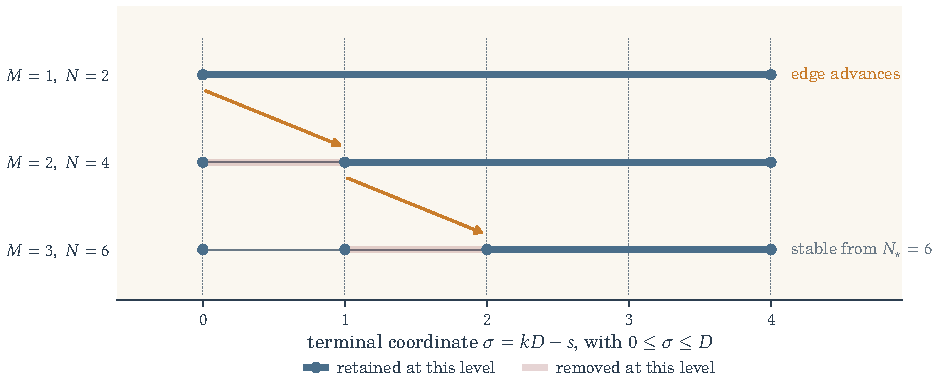
\includegraphics{figs/fig5-erosion-staircase.pdf}
\caption{The integral-defect erosion staircase, drawn in the terminal coordinate
$\sigma=kD-s$ alone; the spectral parameter is recovered by $s=kD-\sigma$, which
reverses orientation. Each row is a constraint level $M=1,\dots,\nu$, first
imposed at cutoff $N=M(k+1)$, and the levels run downward, so the bottom row is
the stable one. At level $M$ the surviving continuous interval is $[M-1,D]$ and
the isolated survivors are $\{0,\dots,M-2\}$: the continuous endpoint advances one
unit per level and leaves the vacated endpoint behind as an isolated point, and
the faded segment is the open interval removed at that level. The staircase halts
at $M=\nu$, that is at $N_*=\nu(k+1)$. Drawn for the Albert step $D=4$ at
$r=\tfrac14$, where $k=1$ and $\nu=3$, so the levels arrive at $N=2,4,6$ and
$N_*=6$. The bottom row is $\sigma\in[2,4]\cup\{0,1\}$, that is
$s\in[0,2]\cup\{3,4\}$, the all-degree locus \eqref{eq:stab}.}
\label{fig:staircase}
\end{figure}

The all-degree locus and the stabilization degree are now corollaries, obtained
by letting the cutoff grow until $M_N$ saturates at $\nu$.

\begin{corollary}[Integral defect leaves one interval and finitely many isolated points]
\label{thm:stab}
Under the hypotheses of \Cref{thm:staircase},
\begin{equation}
  \mathcal{W}_\infty(r,d)
  =\bigl\{\,jD:0\le j<\lfloor r\rfloor\,\bigr\}
  \;\cup\;[\lfloor r\rfloor D,\;rD+1]
  \;\cup\;\bigl\{\,rD+\ell:2\le\ell\le\nu\,\bigr\},
  \label{eq:stab}
\end{equation}
empty pieces omitted: the retained ladder, the surviving band, and the $\nu-1$
isolated spectral zeros above it.
\end{corollary}

\begin{proof}[Proof of \Cref{thm:stab}]
For $N\ge\nu(k+1)$ one has $M_N=\nu$, so \eqref{eq:staircase} is independent of
$N$ and equals $\mathcal{W}_\infty$. Substituting $M_N=\nu$ and $kD-\nu=rD$ turns
$[(k-1)D,kD-\nu+1]$ into $[\lfloor r\rfloor D,rD+1]$, since $(k-1)D=\lfloor
r\rfloor D$, and turns $\{kD-j:0\le j\le\nu-2\}$ into
$\{rD+\ell:2\le\ell\le\nu\}$ under $\ell=\nu-j$. The ladder $\{jD:0\le j\le k-2\}$
is $\{jD:0\le j<\lfloor r\rfloor\}$.
\end{proof}

\subsection{A Critical Rectangle Gives the Exact Stabilization Degree}
\begin{corollary}[A critical rectangle gives the exact stabilization degree]
\label{thm:ncut}
Under the same hypotheses, $\mathcal{W}_N(r,d)=\mathcal{W}_\infty(r,d)$ for every
$N\ge N_*$ and $\mathcal{W}_{N_*-1}\supsetneq\mathcal{W}_\infty(r,d)$, where
\begin{equation}
  N_*\;=\;\nu\,(k+1).
  \label{eq:ncut}
\end{equation}
More precisely, the level-$m$ constraint first appears at cutoff $m(k+1)$: when
$\nu=1$ the capped band is already stable at cutoff $k+1$ and no subsequent band
erosion occurs; when $\nu\ge2$ the first erosion is at $N=2(k+1)$;
and each event $2\le m\le\nu$ lowers the continuous endpoint by one unit and
leaves the old endpoint as an isolated point.
\end{corollary}

\begin{proof}[Proof of \Cref{thm:ncut}]
By \eqref{eq:MN}, $M_N$ is nondecreasing in $N$, reaches $\nu$ exactly at
$N=\nu(k+1)$, and takes the value $m<\nu$ first at $N=m(k+1)$. So
\eqref{eq:staircase} is constant for $N\ge N_*$ and equals $\mathcal{W}_\infty$
by \Cref{thm:stab}.

Suppose first that $\nu=1$, so that $N_*=k+1$ and $N_*-1=k$, a cutoff below the
hypothesis $N\ge k+1$ of \Cref{thm:staircase}; the strictness is therefore argued
directly. At cutoff $k$ every admitted partition has at most $k$ rows, so every
cell lies in a row $i\le k$. Its rank factor $D(r-i+1)+(j-1)$ is at least
$D(r-k+1)=D-\nu=D-1>0$, since $\nu<D$ always, and its spectral factor
$s-(i-1)D+(j-1)$ is at least $s-(k-1)D$, hence nonnegative for
$s\ge(k-1)D$. Thus every pivot is nonnegative there and
$[(k-1)D,\infty)\subseteq\mathcal{W}_k(r,d)$, whereas by \eqref{eq:stab}
$\mathcal{W}_\infty(r,d)\cap[(k-1)D,\infty)=[(k-1)D,kD]$. So
$\mathcal{W}_{N_*-1}\supsetneq\mathcal{W}_\infty$.

Now suppose $\nu\ge2$, so $N_*-1=\nu(k+1)-1\ge k+1$ and \Cref{thm:staircase}
applies at that cutoff, where $M_{N_*-1}=\nu-1$. Its continuous interval
$[(k-1)D,kD-\nu+2]$ ends at $rD+2$ whereas the stable interval ends at $rD+1$, so
the open unit gap $(rD+1,rD+2)$ lies in
$\mathcal{W}_{N_*-1}\setminus\mathcal{W}_\infty$.

Finally, each increment of $M_N$ from $m-1$ to $m$ replaces
$[m-2,D]\cup\{0,\dots,m-3\}$ by $[m-1,D]\cup\{0,\dots,m-2\}$, lowering the
continuous edge by one unit and retaining $m-2$ as an isolated point. That is the
stated erosion event.
\end{proof}

The predicted cutoffs are attained exactly: $N_*=6$ at $(\tfrac32,8)$ and at
$(\tfrac14,8)$, $N_*=8$ at $(\tfrac52,8)$, $N_*=4$ at $(\tfrac12,8)$, and $N_*=2$
at $(\tfrac34,8)$ and $(\tfrac12,4)$. For the Albert step $D=4$ the three
admissible defects give the $3:2:1$ staircase of \Cref{fig:staircase}: with
$m=\lfloor r\rfloor$ and the ladder $\{0,4,\dots,4(m-1)\}$ appended, the terminal
locus is $[4m,4m+2]\cup\{4m+3,4m+4\}$ at $\nu=3$, then $[4m,4m+3]\cup\{4m+4\}$ at
$\nu=2$, then the unbroken $[4m,4m+4]$ at $\nu=1$. As explicit all-degree
instances of \eqref{eq:stab}, rather than finite-cutoff computations, the two
quarter-rank classes at the Albert step give
\begin{equation}
  \mathcal{W}_\infty\!\left(\tfrac12,8\right)=[0,3]\cup\{4\},
  \qquad
  \mathcal{W}_\infty\!\left(\tfrac14,8\right)=[0,2]\cup\{3,4\}.
  \label{eq:half8}
\end{equation}

\subsection{Rational Content Grids Force Stabilization; Irrational Steps
  Remain Open}
\label{sec:nonintegral}

Outside the two exact regimes no closed form is available, but stabilization
itself is not in doubt. It follows from two facts already established: the locus
is caged in a bounded interval, and at rational step every sign change can occur
only on a fixed finite lattice. A decreasing sequence of subsets of a finite
stratification must terminate.

\begin{theorem}{Rational steps stabilize}{ratstab}
Let $d>0$ with $D=\tfrac d2\in\Qq$, and let $r\in\Rr$. Then there is a finite
$N_0=N_0(r,d)$ with
\begin{equation}
  \mathcal{W}_N(r,d)\;=\;\mathcal{W}_\infty(r,d)
  \qquad\text{for every } N\ge N_0 .
  \label{eq:ratstab}
\end{equation}
For $r>0$ nonintegral, $\mathcal{W}_\infty(r,d)$ is a finite union of closed
intervals and isolated points contained in $[0,D\lceil r\rceil]$, with all
endpoints in $b^{-1}\Zint$, where $D=a/b$ in lowest terms.
\end{theorem}

\begin{proof}[Proof of \Cref{thm:ratstab}]
Take first $r>0$ nonintegral and put $k=\lceil r\rceil$, $D=a/b$ in lowest terms.
By \Cref{prop:cap} and \eqref{eq:maxlocus}, together with the exclusion of $s<0$
by the one-box partition $\lambda=(1)$, every $\mathcal{W}_N$ with $N\ge k+1$ is
contained in the bounded interval $[0,kD]$.

By \eqref{eq:interlock} the only $s$-dependence of a pivot is the factor
$F_{\lambda,D}(s)$, whose roots are the cell values $(i-1)D-(j-1)$. Each of these
lies in $b^{-1}\Zint$, since $(i-1)a/b-(j-1)=\bigl((i-1)a-(j-1)b\bigr)/b$.
Consequently every pivot has constant sign on each open interval
$\bigl(\tfrac mb,\tfrac{m+1}{b}\bigr)$, and the finitely many such intervals
meeting $[0,kD]$, together with the finitely many points $\tfrac mb$ in $[0,kD]$,
form a finite stratification $\mathcal{S}$ of that interval into
$2bkD+1$ strata. Each $\mathcal{W}_N\cap[0,kD]$ is a union of members of
$\mathcal{S}$: on an open stratum every pivot is of one sign, so the stratum lies
in $\mathcal{W}_N$ or is disjoint from it.

Finally $\mathcal{W}_{N+1}\subseteq\mathcal{W}_N$, because $\mathcal{W}_N$ is the
intersection of the nonnegativity sets of the pivots of degree at most $N$ and
the index set grows with $N$. A decreasing sequence of subunions of a finite
stratification is eventually constant, and its eventual value is its
intersection, namely $\mathcal{W}_\infty$. Its endpoints are strata boundaries,
hence lie in $b^{-1}\Zint$.

For $r$ a positive integer, \Cref{thm:intrank} gives $\mathcal{W}_N(r,d)$
explicitly and independently of $N$ for $N\ge r$, so $N_0=r$ serves. For $r=0$,
\Cref{prop:rankzero} gives $\mathcal{W}_N(0,d)=\Rr$ at every $N$. For $r<0$, the
pair $(r,d)$ is the image under \Cref{thm:transpose} of the positive pair
$(-rD,4/d)$, whose step $2/d=1/D$ is again rational; since
\eqref{eq:transposeW} holds cutoff by cutoff, stabilization of the positive
partner at $N_0$ gives stabilization of $(r,d)$ at the same $N_0$.
\end{proof}

The argument uses rationality of $D$ only through the finiteness of the
stratification, and that is exactly what fails otherwise: for irrational $D$ the
fractional parts of $tD$ are dense modulo $1$, the content set $\Lambda_D$ is
dense, and no finite stratification of a bounded interval refines every pivot's
sign pattern. Whether finite stabilization nevertheless holds at irrational step
is open.

Two consequences are worth recording, because together they say exactly how much
of the rational case is effective.

\begin{corollary}[Finite certificate]
\label{cor:certificate}
Let $D=\tfrac d2$ be rational and $r\in\Rr$. Then there is a finite family of
partitions $\mathcal F(r,d)$ with
\begin{equation}
  \mathcal{W}_\infty(r,d)
  \;=\;\bigcap_{\lambda\in\mathcal F(r,d)}\bigl\{\,s\in\Rr:\pi_\lambda(s)\ge0\,\bigr\}.
  \label{eq:certificate}
\end{equation}
\end{corollary}

\begin{proof}[Proof of \Cref{cor:certificate}]
By \Cref{thm:ratstab} there is a finite $N_0$ with
$\mathcal W_{N_0}(r,d)=\mathcal W_\infty(r,d)$; take
$\mathcal F(r,d)=\{\lambda:|\lambda|\le N_0\}$ and apply \eqref{eq:loci}.
\end{proof}

\begin{corollary}[The stabilization degree is self-dual]
\label{cor:n0dual}
Write $N_0(r,d)$ for the least cutoff at which \eqref{eq:ratstab} holds. Then
\begin{equation}
  N_0\bigl(-rD,\;\tfrac4d\bigr)\;=\;N_0(r,d)
  \label{eq:n0dual}
\end{equation}
whenever either side is defined.
\end{corollary}

\begin{proof}[Proof of \Cref{cor:n0dual}]
\Cref{thm:transpose} matches $\mathcal W_N(r,d)$ with
$\mathcal W_N(-rD,4/d)$ cutoff by cutoff, since partition conjugation preserves
degree. A cutoff is therefore stabilizing on one side exactly when it is
stabilizing on the other, and the least such cutoffs agree.
\end{proof}

\Cref{cor:certificate} is where the effectivity gap sits: it asserts that a
finite certificate exists without bounding its degree, and determining a
minimal-degree certificate is the open problem recorded in
Section~\ref{sec:scope}. \Cref{cor:n0dual} says that the gap is one problem and
not two, since the reciprocal-step image of an unsettled case is unsettled by
exactly the same amount.

\Cref{thm:ratstab} settles the three examples that the finite-cutoff computations
above leave without a closed form. At $(\tfrac32,6)$, $(\tfrac32,10)$ and
$(\tfrac32,3)$ the steps are $D=3,5,\tfrac32$, all rational, so each locus is
eventually constant. What is not settled for them is the stabilization degree and
the closed form, and that is where the remaining work lies.

The neighbouring chamber shows what integrality of the defect buys. On the open
chamber $0<rD<1$ the sign of every rank factor is constant, since by
\eqref{eq:pivot} each is affine in $rD$ and changes sign only at a lattice point,
i.e.\ at the chamber boundary. Hence the fixed-cutoff locus is the same for all
ranks in the chamber, and the ranks $\tfrac16,\tfrac18,\tfrac1{12},\tfrac1{16}$
at $d=8$ are analytically distinct but positivity-identical, with common locus
$[0,1]\cup\{2,3,4\}$ at cutoff $N=12$. This is not an instance of \eqref{eq:stab}:
the defect there is $\nu=4(1-r)\in(3,4)$, never an integer, so no rank-null ideal
is available and \Cref{thm:stab} does not apply.

\begin{remark}[Nonintegral defect]
\label{rem:nonintegral-nu}
When $\nu\notin\Zint$ there is no critical-row ideal, so \eqref{eq:stab} does not
apply and the master pivot formula \eqref{eq:pivot} remains the exact description.
Two things can then happen that \eqref{eq:stab} does not capture: truncation or
stabilization by a later-row rank-null ideal, at $t>0$ with $\nu+tD\in\Zint$, and
two-sided fragmentation of the band. The case $d\equiv2\pmod4$ at half-integer rank is of this kind: at
$(\tfrac32,10)$, where $\nu=\tfrac52$, the locus at $N=12$ is
$\{0\}\cup\{5\}\cup[7,8]\cup\{9\}\cup\{10\}$, which has several connected
components inside the initial band --- a surviving interval together with
additional isolated interior points --- so no single-band closed form holds. The
pivot formula still locates every sign and zero, and \Cref{thm:ratstab} shows the
locus does stabilize; what is missing is a uniform closed form and a threshold.
\end{remark}

What the exact regimes add beyond \Cref{thm:ratstab} is effectivity. For the
unit-numerator family \Cref{bcor:unitstep} shows that no erosion occurs at any
degree, so $N_0=k+1$; at integral defect \Cref{thm:ncut} gives the exact threshold
$N_*=\nu(\lceil r\rceil+1)$. Outside those two regimes \Cref{thm:ratstab}
guarantees stabilization but does not determine the least stabilizing cutoff, and
nonintegral defect splits further along the middle row of \Cref{tab:regimes}. If
$b\nu\in\Zint$, \Cref{cor:defectideal} supplies a later-row principal rank-null
ideal, which may truncate erosion by a mechanism distinct from the critical-row
staircase. If $b\nu\notin\Zint$, no rank-null ideal exists at any row, so
stabilization must come solely from the finiteness of the rational sign
stratification. The examples $(\tfrac32,6)$, $(\tfrac32,10)$ and $(\tfrac32,3)$
all belong to this latter class. Their computed loci are stationary over the
displayed cutoff ranges --- $10\le N\le14$, $12\le N\le14$ and $12\le N\le14$
respectively --- but those observations do not determine the least stabilizing
cutoff. Determining $N_0$, separately in each of the two nonintegral-defect
classes, is the open problem that replaces the former question of whether
stabilization occurs at all.

\section{Partition Conjugation Transports Positivity Across Reciprocal Steps}
\label{sec:dual}

The pairing at step $d$ and the pairing at the reciprocal step $4/d$ are carried
onto one another by conjugation of partitions. This is the positivity-side
counterpart of the reciprocal-step duality of \Cref{thm:duality}: there the
symbol at step $h$ was matched with the symbol at step $1/h$, and here, since
$h=D$, the same involution $D\mapsto1/D$ acts on the Jack pairing.

\subsection{Conjugation Sends \texorpdfstring{$d$}{d} to \texorpdfstring{$4/d$}{4/d}}

\begin{theorem}{Partition conjugation transports the locus under $d\leftrightarrow4/d$}{transpose}
Let $d>0$ and $D=d/2$, put $d^{\vee}=4/d$ so that $D^{\vee}=1/D$, and write
$\lambda'$ for the conjugate partition. Then for every partition $\lambda$ and
every $y$,
\begin{equation}
  F_{\lambda',D^{\vee}}\!\left(-\tfrac{y}{D}\right)
  \;=\;\left(-\tfrac1D\right)^{|\lambda|}F_{\lambda,D}(y).
  \label{eq:transposeF}
\end{equation}
Consequently, setting $r^{\vee}=-rD$, the pivots at $(r,d)$ and at
$(r^{\vee},d^{\vee})$ have equal signs under $\lambda\mapsto\lambda'$ and
$s\mapsto-s/D$, and therefore, at every cutoff $N$ and hence for the all-degree
locus,
\begin{equation}
  \mathcal{W}_N\!\left(-rD,\;\tfrac4d\right)
  \;=\;-\tfrac1D\,\mathcal{W}_N(r,d).
  \label{eq:transposeW}
\end{equation}
The correspondence $(r,d)\mapsto(-rD,4/d)$ is an involution.
\end{theorem}

\begin{proof}[Proof of \Cref{thm:transpose}]
The cells of $\lambda'$ are exactly the pairs $(j,i)$ with $(i,j)\in\lambda$. The
cell $(j,i)$ contributes to the left side of \eqref{eq:transposeF} the factor
\begin{equation*}
  -\tfrac{y}{D}-(j-1)D^{\vee}+(i-1)
  \;=\;-\tfrac{y}{D}-\tfrac{j-1}{D}+(i-1)
  \;=\;-\tfrac1D\bigl(y-(i-1)D+(j-1)\bigr),
\end{equation*}
which is $-1/D$ times the factor contributed by $(i,j)$ to $F_{\lambda,D}(y)$;
taking the product over all $|\lambda|$ cells gives \eqref{eq:transposeF}.
Applying it at $y=rD$, and noting $r^{\vee}D^{\vee}=(-rD)(1/D)=-r=-rD/D$, gives
$F_{\lambda',D^{\vee}}(r^{\vee}D^{\vee})=(-1/D)^{|\lambda|}F_{\lambda,D}(rD)$;
applying it at $y=s$ gives
$F_{\lambda',D^{\vee}}(-s/D)=(-1/D)^{|\lambda|}F_{\lambda,D}(s)$. By
\eqref{eq:pivot} the numerator of the dual pivot is $D^{-2|\lambda|}$ times that
of the original, while its denominator is
$(D^{\vee})^{|\lambda|}H_{\lambda'}(D^{\vee})=D^{-|\lambda|}H_{\lambda'}(D^{\vee})$.
Hence
\begin{equation}
  \pi^{(r^{\vee},D^{\vee})}_{\lambda'}\!\Bigl(-\frac{s}{D}\Bigr)
  \;=\;\frac{H_\lambda(D)}{H_{\lambda'}(D^{\vee})}\;\pi^{(r,D)}_{\lambda}(s),
  \label{eq:hookratio}
\end{equation}
and both hook products are positive by \eqref{eq:hook}, so the two pivots have
the same sign. Note that the dual hook is $H_{\lambda'}(D^{\vee})$, evaluated at
the dual parameter.
Conjugation preserves $|\lambda|$ and is an involution on partitions of each
size, so the correspondence is a bijection of the constraint sets at each cutoff,
giving \eqref{eq:transposeW}. Finally $-r^{\vee}D^{\vee}=rD\cdot\tfrac1D=r$
and $4/d^{\vee}=d$, so the correspondence is an involution.
\end{proof}

The involution $d\mapsto4/d$ fixes $d=2$, exchanges
$d=1$ with $d=4$, and carries $d=8$ to the formal step $\tfrac12$. Among the
multiplicities of simple Euclidean Jordan algebras of rank at least $3$ it
therefore permutes $\{1,2,4\}$ and moves the exceptional rank-$3$ value $d=8$
outside the Jordan range altogether: the dual of the Albert cell is formal. The
transpose duality is thus visible on the geometric axis only for $d\in\{1,2,4\}$.
\subsection{Positive-Rank Loci Determine Their Negative-Rank Images}
Transporting \Cref{thm:stab} through \eqref{eq:transposeW} supplies
negative-rank loci, which the positive-rank argument does not reach directly: for $r>0$ nonintegral with $\nu\in\Zint_{>0}$,
\begin{equation}
  \mathcal{W}_\infty\!\left(-rD,\tfrac4d\right)
  =\bigl\{-j:0\le j<\lfloor r\rfloor\bigr\}
  \cup\Bigl[-r-\tfrac1D,\;-\lfloor r\rfloor\Bigr]
  \cup\Bigl\{-r-\tfrac{\ell}{D}:2\le\ell\le\nu\Bigr\}.
  \label{eq:negstab}
\end{equation}
Formula \eqref{eq:negstab} is the transport of one result only.
\Cref{thm:transpose} transports every positive-rank statement of the preceding
sections: chamber positivity, the universal retained grid, the unit-numerator
loci, the integral-defect classification and every finite-cutoff locus all have
negative-rank images. What \eqref{eq:negstab} supplies is the closed form, and
that is what requires the dual pair to have integral defect. The universal grid
of \Cref{prop:grid}, by contrast, dualizes with no hypothesis on the defect: for
real $\rho<0$ and $d>0$ with $D=\tfrac{d}{2}$,
\begin{equation}
  \bigl\{-j\;:\;0\le j\le\lceil-\rho D\rceil\bigr\}
  \;\subseteq\;\mathcal{W}_\infty(\rho,d),
  \label{eq:neggrid}
\end{equation}
since the positive partner of $(\rho,d)$ under \Cref{thm:transpose} is
$(-\rho D,4/d)$, whose retained grid $\{jD^{\vee}\}$ maps to $\{-j\}$. A
dualized cell chamber is likewise retained whenever the reciprocal step is
rational. What does fail is the naive guess that the negative side is a
reflection of the positive band. At
\begin{equation}
  r=-\tfrac32,\qquad d=1,\qquad s=-\tfrac38,\qquad \lambda=(2,2),
  \label{eq:negwitness}
\end{equation}
one finds $F_{\lambda,D}(rD)<0$ and $F_{\lambda,D}(s)>0$, so the pivot is
strictly negative at a point a reflected band would have retained. Under
\Cref{thm:transpose} this cell is dual to $(\tfrac34,4)$, whose defect
$\tfrac12$ is not an integer; it therefore lies outside \eqref{eq:negstab},
exactly as the failure requires.
No uniform closed formula is established for arbitrary negative rank.
\eqref{eq:negstab} treats exactly the negative cells dual to positive integral
defect, and \Cref{thm:transpose} transports the chamber, retained-grid,
unit-numerator and finite-cutoff results; a general all-degree formula at
negative rank is left open.

\subsection{Rank Zero Annihilates Every Nonconstant Mode}
The master pivot formula \eqref{eq:pivot} is an algebraic identity in $r$, so it
survives the passage to $r=0$ even though the order-dependent apparatus of this
section --- the defect, the floors and ceilings, the band --- does not. Exactly one
clean statement is available at the wall itself.

\begin{proposition}{Rank zero annihilates every nonconstant mode}{rankzero}
Let $d>0$ and $r=0$. Every nonempty partition $\lambda$ contains the cell
$(1,1)$, so $F_{\lambda,D}(0)=0$. Hence
\begin{equation}
  \pi_\lambda(s)=0\qquad(\lambda\ne\varnothing)
  \label{eq:vacuum}
\end{equation}
for every real $s$. Thus every cutoff Gram form is positive semidefinite for
every $s$, but its entire nonconstant sector is null; only the empty-partition
mode survives.
\end{proposition}

This is the positivity-side image of the shift quotient's value $\Rm_{0,h}(s)=1$ from
\Cref{thm:shift}: the empty product read two ways, analytically a unit and
functionally null. It is a statement about $r=0$ alone, and it is consistent with
\Cref{thm:transpose}, which fixes $r=0$ for every $d$. No neighbourhood formula
for $r<0$ may be inferred from it, and none is asserted here.

\section{Positivity Survives Where Polynomial Carriers Do Not}
\label{sec:scope}

The two halves of the paper answer different realizability questions, and the
fractional-rank positivity computed above is where they part company. The
separation can be stated as a single result, each clause of which is a
specialization of a theorem already proved.

\subsection{The Separation}

\begin{corollary}[Analytic existence, polynomial realizability and positivity separate]
\label{cor:separation}
Fix $d>0$, put $D=\tfrac d2$, and let $r\in\Rr\setminus\Zint_{\ge0}$. Then
\begin{enumerate}
\item[(i)] $\Gc_D(r,\cdot)$ is meromorphic on $\Cc$;
\item[(ii)] its spectral shift quotient admits no polynomial Bernstein--Sato
  datum affine-compatible with it in the sense of \eqref{eq:affinecompat};
\item[(iii)] the formal Jack--Riesz pairing is positive semidefinite at $s=rD$ at
  every cutoff.
\end{enumerate}
If $rD\notin\Lambda_D$ the pairing is positive definite at $s=rD$ at every
cutoff; if $rD\in\Lambda_D$ the corresponding principal rank-null ideal of
\Cref{prop:idealfull} appears from its minimal rectangle degree onward, and the
pairing is definite only after quotienting it.
\end{corollary}

\begin{proof}[Proof of \Cref{cor:separation}]
Part (i) is \Cref{def:symbol}. Part (ii) is \Cref{prop:bernstein}, whose conclusion
$r\in\Zint_{\ge0}$ is excluded by hypothesis. For (iii), specialize
\eqref{eq:pivot} at $s=rD$: the two factors coincide, so
\begin{equation*}
  \pi_\lambda(rD)\;=\;\frac{F_{\lambda,D}(rD)^{2}}{D^{|\lambda|}H_\lambda(D)}\;\ge\;0
\end{equation*}
for every $\lambda$, since $H_\lambda(D)>0$. This is \eqref{eq:balanced}. The
pivot vanishes exactly when $F_{\lambda,D}(rD)=0$, that is when $\lambda$ contains
a cell of content $rD$, which requires $rD\in\Lambda_D$; the vanishing modes are
then the principal ideal of \Cref{prop:idealfull}.
\end{proof}

The continuation thus separates three notions that coincide on symmetric cones:
analytic existence, polynomial realizability, and positivity. The
Barnes--Gindikin symbol exists at every complex factor count. Its spectral
recurrence terminates polynomially only at nonnegative integral rank. The formal
Jack--Riesz pairing, however, can remain positive semidefinite at nonintegral
rank.

\subsection{Interpretation and Limitations}

Fractional rank does not force loss of positivity. At rational steps whose
rescaled rank lies inside a cell chamber, \Cref{thm:chamber} gives a nontrivial
positive interval; the integral-defect cases of \Cref{thm:stab} supply further
semidefinite intervals on the lattice. A single example such as
$(r,d)=(\tfrac32,2)$ already proves the intended claim that positivity does not
force integrality. The definiteness must nevertheless be stated carefully. At
$(\tfrac32,2)$ the open band is positive \emph{definite}, by \Cref{thm:d2}. At
$(\tfrac32,4)$ definiteness depends on the cutoff: $\alpha=\tfrac12$ puts the cell
$(3,2)$ in the rank-null ideal, so every $\lambda$ with $\lambda_3\ge2$ is
identically null, minimally $(2,2,2)$. That partition first fits at $N=6$, so for
$N<6$ the open band is positive definite, while for $N\ge6$ it is semidefinite but
not definite and becomes definite only after quotienting the ideal. Either way the
fractional-rank positivity is compatible with quotient or non-polynomial
realizations, but does not construct one. It therefore does not conflict with
\Cref{prop:bernstein}, which obstructs compatible \emph{polynomial}
Bernstein--Sato realizations rather than positive forms.

Two limits on what the positivity statements assert should be recorded. Every
finite-cutoff locus above is indexed by its cutoff; the unindexed
$\mathcal W_\infty$ is the separately defined all-degree locus, obtained by
requiring nonnegativity at every cutoff, and finite-cutoff nullities must not be
read as unindexed infinite-dimensional nullities. And positivity of this formal
pairing is not the existence of a Euclidean Jordan algebra, a symmetric cone, or a
determinant carrier; the pair $(r,d)=(3,6)$ used here is formal, as recorded
after \Cref{prop:cbtype}. The fractional case displayed at $d=6$ is also the most
fragile: it has no protecting ideal, and
its band erodes from both ends. The same step at \emph{integer} rank $3$ is a
useful contrast: by \Cref{thm:intrank} its positive locus is
$\{0\}\cup\{3\}\cup[6,\infty)$ at every cutoff $N\ge3$ --- exactly the shape of a
rank-$3$ Wallach set with $\tfrac d2=3$, although no Euclidean Jordan algebra has
$(r,d)=(3,6)$. Integrality of the \emph{rank}, not realizability of the pair
$(r,d)$, is what the positivity computation tracks.

\begin{remark}[Cap points are not classical ladder points]
\label{rem:isolated}
In the computed finite-degree loci the points $8$ at $(\tfrac32,8)$, $6$ at
$(\tfrac32,6)$ and $12$ at $(\tfrac52,8)$ arise as exact Pochhammer zeros: points
where the critical rectangle pivot vanishes rather than changes sign. Each of the
three is the cap $D\lceil r\rceil$, so all three are retained at every degree by
\Cref{prop:grid}, and by \eqref{eq:maxlocus} each is the maximum of its
all-degree locus. At integral defect \Cref{thm:stab} additionally identifies them
inside the complete closed form. They are therefore formal fractional analogues of
the discrete Wallach points, produced by a different mechanism from the classical
discrete points below the band, which arise from the ladder. At $(\tfrac32,6)$,
whose defect is not integral, the point $6$ is still all-degree and isolated ---
the degree-six census already excludes $(5,6)$ --- although the complete locus
below it remains unclassified.
\end{remark}

\subsection{Open Problems}

The remaining question is not whether fractional rank is analytically meaningful,
but whether its positive forms admit a natural nonpolynomial carrier. Three
directions remain open. The first is the effective content of
\Cref{thm:ratstab}: the stabilization degree and the closed form at rational
nonintegral defect, where stabilization is now known to occur but no threshold is
available; equivalently, a minimal-degree certificate for the finite family of
\Cref{cor:certificate}. The second is whether finite stabilization holds at all at
irrational step, where the content set is dense and the stratification argument of
\Cref{thm:ratstab} has nothing to work with. The third is a complete description
of the negative-rank loci, beyond the positive-rank families that
\Cref{thm:transpose} transports. By \Cref{cor:n0dual} the first and third are not
independent: the reciprocal-step image of an unsettled rational case is unsettled
at exactly the same cutoff.

A fourth is the carrier question in its kernel form. \Cref{prop:collapse} shows
that at a discrete Wallach point the reproducing kernel \eqref{eq:bergman}
collapses onto a model in finitely many variables, and at integer rank the number
of variables is the rank of the orbit carrying the corresponding Riesz measure
\cite[Prop.~VII.2.3]{FK}. That is an identity between two indices, established
here for the formal model only. What is not established, and is the natural
successor to \Cref{prop:bernstein}, is whether any genuine Hilbert space of
functions reproduces $B_{N,r,s}$ at nonintegral $r$ --- a carrier for the
fractional Wallach set that is a kernel rather than a determinant.
\Cref{prop:bernstein} obstructs the polynomial determinant carrier; it says
nothing about a reproducing one, and the positivity computed in
Sections~\ref{sec:wallach}--\ref{sec:arith} is exactly the hypothesis such a
carrier would need.

\bigskip
\noindent\textbf{Supplementary material.} The exact-arithmetic verification
code, figure sources, environment lockfile, SHA-256 manifest, and finite-cutoff
data for this revision are release v1.1.0 of
\href{https://github.com/johnzfitch/gindikin-rank}{\texttt{github.com/johnzfitch/gindikin-rank}},
archived under DOI
{\urlstyle{same}\href{https://doi.org/10.5281/zenodo.21713316}{\nolinkurl{10.5281/zenodo.21713316}}},
which also covers the earlier revision (v1.0.0). The script
\texttt{ancillary\_census.py} emits the three quantitative receipts that
\Cref{sec:erosion} leaves to the supplement, and \texttt{verify\_positivity.py}
recomputes all displayed loci, erosion degrees, and tabulated finite-cutoff
examples of Sections~\ref{sec:wallach}--\ref{sec:dual} by exact cell
decomposition and exhaustive partition checks. The scripts verify the stated
computational instances; the analytic proofs and the identifications with the
literature do not depend on them.

\appendix

\section{Notation Crosswalk with Ruijsenaars's Multiple Zeta}
\label{app:ruij}

\Cref{lem:sector} imports one analytic fact from \cite{Ruij}. Ruijsenaars writes
$\zeta_N(s,w\mid a_1,\dots,a_N)$ for the multiple zeta function and builds it
from $f(t)=t^{N}\prod_{j=1}^{N}(1-e^{-a_jt})^{-1}$ \cite[(3.1)]{Ruij}. The
present case is $N=2$ with $a_1=1$ and $a_2=h$, so that $f(t)=t^{2}K(t)$ for the
kernel $K$ of \eqref{eq:mellin}. Under that specialization the dictionary is the
following.

\begin{center}
\small
\begin{tabular}{@{}l l l@{}}
\toprule
\estabhead{Ruijsenaars \cite{Ruij}} & \estabhead{Here} & \estabhead{Where}\\
\midrule
$N$, $(a_1,a_2)$ & $2$, $(1,h)$ & \eqref{eq:mellin}\\
$f(t)=t^{N}\prod_j(1-e^{-a_jt})^{-1}$ & $t^{2}K(t)$ & \cite[(3.1)]{Ruij}\\
$s$ & $z$ & \eqref{eq:mellin}\\
$w$ & $a$ & \eqref{eq:mellin}\\
$\zeta_2(s,w\mid1,h)$ & $\Zt(z,a\mid1,h)$ & \eqref{eq:mellin}\\
$\Psi_N(w)=\partial_s\zeta_N(s,w)\big|_{s=0}$ & $\Fh(a)$ & \cite[(3.12)]{Ruij}\\
truncation order $M'$ & $M+2$ & \eqref{eq:zetaexp}\\
Taylor coefficients of $f$ through $M'$ & $c_n(h)$ for $n\le M'-2$ & \eqref{eq:zetaexp}\\
remainder (3.14) & $\rho_M(z,a)$ & \Cref{lem:sector}\\
bound (3.15), $O(|w|^{\,N-M'-1})$ & $O(\lvert a\rvert^{-M-1})$ & \Cref{lem:sector}\\
logarithmic coefficient $-\tfrac12B_{2,2}(w)$ & $-Q_h(a)$ & \Cref{thm:duality}\\
\bottomrule
\end{tabular}
\end{center}

\smallskip
\noindent
Two consequences are worth stating explicitly. First, because $\Psi_N$ is already
the $z$-derivative at $z=0$, the expansion \cite[(3.13)]{Ruij} is the
differentiated one and no further passage through $\partial_z$ is needed. Second,
the truncation indices differ by $N=2$: he subtracts the Taylor coefficients of
$f$ through order $M'$, which are the $c_n(h)$ of \eqref{eq:zetaexp} for
$n\le M'-2$, so $M'=M+2$ and his $O(|w|^{\,N-M'-1})$ is our
$O(\lvert a\rvert^{-M-1})$.

\begin{thebibliography}{99}

\bibitem{Barnes} E.~W.~Barnes,
\emph{On the theory of the multiple gamma function},
Trans.\ Cambridge Philos.\ Soc.\ \textbf{19} (1904), 374--425.

\bibitem{Bjork} J.-E.~Bj\"ork,
\emph{Rings of Differential Operators},
North-Holland Mathematical Library \textbf{21},
North-Holland, Amsterdam, 1979.

\bibitem{BO} A.~Borodin, G.~Olshanski,
\emph{$z$-Measures on partitions and their scaling limits},
European J.\ Combin.\ \textbf{26} (2005), no.~6, 795--834;
preprint arXiv:math-ph/0210048.

\bibitem{Boas} R.~P.~Boas,
\emph{Entire Functions},
Pure and Applied Mathematics \textbf{5}, Academic Press, New York, 1954.

\bibitem{DGR} H.~Ding, K.~I.~Gross, D.~St.~P.~Richards,
\emph{Ramanujan's master theorem for symmetric cones},
Pacific J.\ Math.\ \textbf{175} (1996), 447--490.

\bibitem{FK} J.~Faraut, A.~Kor\'anyi,
\emph{Analysis on Symmetric Cones},
Oxford Mathematical Monographs, Clarendon Press, Oxford, 1994.

\bibitem{FR} E.~Friedman, S.~Ruijsenaars,
\emph{Shintani--Barnes zeta and gamma functions},
Adv.\ Math.\ \textbf{187} (2004), 362--395.

\bibitem{Ruij} S.~N.~M.~Ruijsenaars,
\emph{On Barnes' multiple zeta and gamma functions},
Adv.\ Math.\ \textbf{156} (2000), no.~1, 107--132.

\bibitem{Gindikin} S.~G.~Gindikin,
\emph{Analysis in homogeneous domains},
Russian Math.\ Surveys \textbf{19} (1964), 1--89.

\bibitem{Kimura} T.~Kimura,
\emph{Introduction to Prehomogeneous Vector Spaces},
Translations of Mathematical Monographs \textbf{215},
American Mathematical Society, Providence, 2003.

\bibitem{LM} J.~M.~Landsberg, L.~Manivel,
\emph{The sextonions and $E_{7\frac12}$},
Adv.\ Math.\ \textbf{201} (2006), no.~1, 143--179.

\bibitem{Macdonald} I.~G.~Macdonald,
\emph{Symmetric Functions and Hall Polynomials}, 2nd ed.,
Oxford Mathematical Monographs, Clarendon Press, Oxford, 1995; Ch.~VI, \S10.

\bibitem{Petrov} L.~Petrov,
\emph{The Jack $z$-measures and their degenerations},
\texttt{arXiv:1111.3399}.

\bibitem{PerezMarco} R.~P\'erez-Marco,
\emph{On the definition of higher Gamma functions},
Constr.\ Approx.\ \textbf{61} (2025), 413--443.

\bibitem{Stanley} R.~P.~Stanley,
\emph{Some combinatorial properties of Jack symmetric functions},
Adv.\ Math.\ \textbf{77} (1989), 76--115.

\bibitem{TW} L.~Tizzano, J.~Winding,
\emph{Multiple sine, multiple elliptic gamma functions and rational cones},
preprint, arXiv:1502.05996.

\bibitem{Westbury} B.~W.~Westbury,
\emph{Sextonions and the magic square},
J.\ London Math.\ Soc.\ (2) \textbf{73} (2006), no.~2, 455--474.

\bibitem{Winding} J.~Winding,
\emph{Multiple elliptic gamma functions associated to cones},
Adv.\ Math.\ \textbf{325} (2018), 56--86; preprint arXiv:1609.02384.

\end{thebibliography}

\end{document}

